%
% File    : sample_dphil_thesis.tex
% Author  : Mauricio Villarroel
% Created : Sept 6, 2013
% ____________________________________________________________________________
%
% Copyright (C) 2013-2022 Mauricio Villarroel. All rights reserved.
%
% SPDX-License-Identifer:  GPL-2.0-only
% ____________________________________________________________________________
%\\
% DESCRIPTION :
%
% Sample DPhil thesis of the Engineering department of 
% the University of Oxford
% ____________________________________________________________________________

\documentclass{oxengthesis}
\usepackage{xfrac}

%
% Document metadata
%


\title       {Local Power Spectra of the Earth's atmosphere}
\author      {Salah Kouhen}
\college     {Linacre College}
\supervisor  {Professor Hannah M. Christensen, Professor David P. Marshall}
\date        {Michaelmas Term, 2024}
\department{Department of Physics, AOPP}


%
% Document contents
%


\makeglossaries

\begin{document}

\frontmatter
\makefrontmatterpages

\mainmatter


% Remove the following line when you are creating your document.
% It only contains the documentation of the OxEngThesis class
%\setcounter{chapter}{-1}
\chapter{The OxEngThesis \latex class}



\begin{OxWarningBox}{IMPORTANT NOTE}
This chapter contains a summary of some of the features available in the \verb|OxEngThesis| class. It is included just to showcase how to use the available formatting options in a \latex source file.

Remove this chapter when you are writing your own thesis or report. It is numbered as ``\verb|Chapter 0|'' so not to change the flow of the rest of the document.
\end{OxWarningBox}


\section{Introduction}


This repository contains a \latex class (OxEngThesis) to write formal academic documents for a student of the Department of Engineering Science at the University of Oxford. For example, my undergraduate students have used this class to write 4$^{th}$-year project (4YP) reports. My doctoral students have typically used this class to write their 1$^{st}$-year Transfer of Status report, 2$^{nd}$-year Confirmation of Status report and their final DPhil thesis. The typical 4YP report contains around 50 pages, whereas a doctoral thesis is a much larger document.

Although I originally created this class for a student at Oxford, I also included in this repository some examples for a PhD thesis for the Massachusetts Institute of Technology and (cough, cough) the University of Cambridge. It should be easy for you to adjust this class to suit the requirements of your academic institution.

LaTex itself is very portable. However, I developed this class under Linux and macOS environments using the latest LaTeX distributions. I have not tested compiling a LaTeX document in Microsoft Windows, but some of my students reported that it works. If you find any problems for Windows, please report any issues to me. Event better, I encourage you to contribute your fixes.

As a research student, a proportion of your time will be devoted to writing science in a formal academic style. There are many resources that will help you to write your thesis, such as ``Writing your thesis''\footnote{\url{https://www.mpls.ox.ac.uk/training/resources-for-researcher-and-career-development/completing-your-dphil/writing-up-your-thesis}}, ``Completing your doctorate''\footnote{\url{https://www.vitae.ac.uk/doing-research/doing-a-doctorate/completing-your-doctorate}}, ``Essay and dissertation writing skills''\footnote{\url{https://www.ox.ac.uk/students/academic/guidance/skills/essay}} and also ``Resources for new students''\footnote{\url{https://cameralab.eng.ox.ac.uk/resources_new_students.html}}. Steven Pinker's talk on ``Linguistics, Style and Writing in the 21st Century''\footnote{\url{https://youtu.be/OV5J6BfToSw}} will provide you with sound advice on writing. 

My students have found very helpful to use the LaTeX typesetting system to write reports, theses, journal papers or other academic documents. You can write your LaTeX documents from scratch, however, it is often easier to start with an already written class template. This way you can focus on (as your supervisor expects) writing about your exciting research contributions, rather than spending time formatting your document or applying other cosmetic changes that just waste everybody's time and distract the reader. 

The OxEngThesis class is based on the \textit{memoir}\footnote{\url{https://ctan.org/pkg/memoir}} package, with the addition of several other packages and extra features useful to format a typical academic document. The main class file is \verb|oxengthesis.cls|. One sample source file is provided (\verb|sample_dphil_thesis.tex|). You can check this sample
PDF file to review an example of the output of a doctoral thesis.

In this chapter, I will summarise some of the features available in the OxEngThesis class. Take a look at the \verb|oxengthesis.cls| file and the rest of this sample thesis document for a more complete overview.


\section{Requirements}


There are several options for writing in LaTeX, including online versions such as Overleaf. I don't recommend online editors, as you will be writing long documents with several figures, tables and other elements. In my experience, having LaTeX installed locally in your computer is a better option.

You will need a modern LaTeX compiler installed in your system, at minimum version 2017. Most modern operating systems use \textit{TexLive}\footnote{\url{https://www.tug.org/texlive}} as the preferred LaTeX typesetting system. If you are using Linux, TexLive is already pre-installed or is readily available from your distribution's software repository (for example Fedora\footnote{\url{https://docs.fedoraproject.org/en-US/neurofedora/latex}} or Ubuntu\footnote{\url{https://help.ubuntu.com/community/LaTeX}}). For macOS, you can download and install the latest MacTeX distribution\footnote{\url{https://tug.org/mactex}}. For Microsoft Windows, follow the installation instructions described in TexLive\footnote{\url{https://tug.org/texlive/windows.html}}.

Install the \textit{Carlito} font\footnote{\url{https://ctan.org/tex-archive/fonts/carlito}} (if it's not already installed in your system). Follow the instructions for your particular operating system in the \verb|./fonts/| directory in this repository. If you are using Microsoft Windows, also install the ``\textit{Latin Modern Math}''\footnote{\url{https://ctan.org/tex-archive/fonts/lm-math}} font, also available in the \verb|./fonts/| directory in this repository.


\section{LaTeX editors}


There are several editors available that will make your life easier when writing LaTeX documents and, ultimately, generating the final PDF file (a.k.a compiling the LaTeX source files). For macOS and iOS, Texifier\footnote{\url{https://www.texifier.com}} works really well. Good editors for Linux are Kile\footnote{\url{https://apps.kde.org/en-gb/kile}} and TeXMaker\footnote{\url{https://www.xm1math.net/texmaker}}. If you know what software is good for Microsoft Windows, let me know so I can add it to my recommendation list.

The LaTeX files in this repository require the \textit{LuaLaTeX}\footnote{\url{https://en.wikipedia.org/wiki/LuaTeX}} engine. You editor should allow you to configure LuaLaTeX as the typesetting engine for your document and automatically take care of the compilation process to generate the final PDF document.


\section{Writing your thesis}


\subsection{Preparing your document}

After you installed your preferred \latex editor, make a copy of the \verb|sample_thesis.tex| sample file provided in this repository. Throughout this tutorial, I will call this new file your ``\textit{main LaTeX source file}''. From your ``\textit{main LaTeX source file}'', remove the line that includes this chapter. It is a line similar to:


\begin{lstlisting}[style=custom-latex]
\setcounter{chapter}{-1}
\chapter{The OxEngThesis \latex class}



\begin{OxWarningBox}{IMPORTANT NOTE}
This chapter contains a summary of some of the features available in the \verb|OxEngThesis| class. It is included just to showcase how to use the available formatting options in a \latex source file.

Remove this chapter when you are writing your own thesis or report. It is numbered as ``\verb|Chapter 0|'' so not to change the flow of the rest of the document.
\end{OxWarningBox}


\section{Introduction}


This repository contains a \latex class (OxEngThesis) to write formal academic documents for a student of the Department of Engineering Science at the University of Oxford. For example, my undergraduate students have used this class to write 4$^{th}$-year project (4YP) reports. My doctoral students have typically used this class to write their 1$^{st}$-year Transfer of Status report, 2$^{nd}$-year Confirmation of Status report and their final DPhil thesis. The typical 4YP report contains around 50 pages, whereas a doctoral thesis is a much larger document.

Although I originally created this class for a student at Oxford, I also included in this repository some examples for a PhD thesis for the Massachusetts Institute of Technology and (cough, cough) the University of Cambridge. It should be easy for you to adjust this class to suit the requirements of your academic institution.

LaTex itself is very portable. However, I developed this class under Linux and macOS environments using the latest LaTeX distributions. I have not tested compiling a LaTeX document in Microsoft Windows, but some of my students reported that it works. If you find any problems for Windows, please report any issues to me. Event better, I encourage you to contribute your fixes.

As a research student, a proportion of your time will be devoted to writing science in a formal academic style. There are many resources that will help you to write your thesis, such as ``Writing your thesis''\footnote{\url{https://www.mpls.ox.ac.uk/training/resources-for-researcher-and-career-development/completing-your-dphil/writing-up-your-thesis}}, ``Completing your doctorate''\footnote{\url{https://www.vitae.ac.uk/doing-research/doing-a-doctorate/completing-your-doctorate}}, ``Essay and dissertation writing skills''\footnote{\url{https://www.ox.ac.uk/students/academic/guidance/skills/essay}} and also ``Resources for new students''\footnote{\url{https://cameralab.eng.ox.ac.uk/resources_new_students.html}}. Steven Pinker's talk on ``Linguistics, Style and Writing in the 21st Century''\footnote{\url{https://youtu.be/OV5J6BfToSw}} will provide you with sound advice on writing. 

My students have found very helpful to use the LaTeX typesetting system to write reports, theses, journal papers or other academic documents. You can write your LaTeX documents from scratch, however, it is often easier to start with an already written class template. This way you can focus on (as your supervisor expects) writing about your exciting research contributions, rather than spending time formatting your document or applying other cosmetic changes that just waste everybody's time and distract the reader. 

The OxEngThesis class is based on the \textit{memoir}\footnote{\url{https://ctan.org/pkg/memoir}} package, with the addition of several other packages and extra features useful to format a typical academic document. The main class file is \verb|oxengthesis.cls|. One sample source file is provided (\verb|sample_dphil_thesis.tex|). You can check this sample
PDF file to review an example of the output of a doctoral thesis.

In this chapter, I will summarise some of the features available in the OxEngThesis class. Take a look at the \verb|oxengthesis.cls| file and the rest of this sample thesis document for a more complete overview.


\section{Requirements}


There are several options for writing in LaTeX, including online versions such as Overleaf. I don't recommend online editors, as you will be writing long documents with several figures, tables and other elements. In my experience, having LaTeX installed locally in your computer is a better option.

You will need a modern LaTeX compiler installed in your system, at minimum version 2017. Most modern operating systems use \textit{TexLive}\footnote{\url{https://www.tug.org/texlive}} as the preferred LaTeX typesetting system. If you are using Linux, TexLive is already pre-installed or is readily available from your distribution's software repository (for example Fedora\footnote{\url{https://docs.fedoraproject.org/en-US/neurofedora/latex}} or Ubuntu\footnote{\url{https://help.ubuntu.com/community/LaTeX}}). For macOS, you can download and install the latest MacTeX distribution\footnote{\url{https://tug.org/mactex}}. For Microsoft Windows, follow the installation instructions described in TexLive\footnote{\url{https://tug.org/texlive/windows.html}}.

Install the \textit{Carlito} font\footnote{\url{https://ctan.org/tex-archive/fonts/carlito}} (if it's not already installed in your system). Follow the instructions for your particular operating system in the \verb|./fonts/| directory in this repository. If you are using Microsoft Windows, also install the ``\textit{Latin Modern Math}''\footnote{\url{https://ctan.org/tex-archive/fonts/lm-math}} font, also available in the \verb|./fonts/| directory in this repository.


\section{LaTeX editors}


There are several editors available that will make your life easier when writing LaTeX documents and, ultimately, generating the final PDF file (a.k.a compiling the LaTeX source files). For macOS and iOS, Texifier\footnote{\url{https://www.texifier.com}} works really well. Good editors for Linux are Kile\footnote{\url{https://apps.kde.org/en-gb/kile}} and TeXMaker\footnote{\url{https://www.xm1math.net/texmaker}}. If you know what software is good for Microsoft Windows, let me know so I can add it to my recommendation list.

The LaTeX files in this repository require the \textit{LuaLaTeX}\footnote{\url{https://en.wikipedia.org/wiki/LuaTeX}} engine. You editor should allow you to configure LuaLaTeX as the typesetting engine for your document and automatically take care of the compilation process to generate the final PDF document.


\section{Writing your thesis}


\subsection{Preparing your document}

After you installed your preferred \latex editor, make a copy of the \verb|sample_thesis.tex| sample file provided in this repository. Throughout this tutorial, I will call this new file your ``\textit{main LaTeX source file}''. From your ``\textit{main LaTeX source file}'', remove the line that includes this chapter. It is a line similar to:


\begin{lstlisting}[style=custom-latex]
\setcounter{chapter}{-1}
\chapter{The OxEngThesis \latex class}



\begin{OxWarningBox}{IMPORTANT NOTE}
This chapter contains a summary of some of the features available in the \verb|OxEngThesis| class. It is included just to showcase how to use the available formatting options in a \latex source file.

Remove this chapter when you are writing your own thesis or report. It is numbered as ``\verb|Chapter 0|'' so not to change the flow of the rest of the document.
\end{OxWarningBox}


\section{Introduction}


This repository contains a \latex class (OxEngThesis) to write formal academic documents for a student of the Department of Engineering Science at the University of Oxford. For example, my undergraduate students have used this class to write 4$^{th}$-year project (4YP) reports. My doctoral students have typically used this class to write their 1$^{st}$-year Transfer of Status report, 2$^{nd}$-year Confirmation of Status report and their final DPhil thesis. The typical 4YP report contains around 50 pages, whereas a doctoral thesis is a much larger document.

Although I originally created this class for a student at Oxford, I also included in this repository some examples for a PhD thesis for the Massachusetts Institute of Technology and (cough, cough) the University of Cambridge. It should be easy for you to adjust this class to suit the requirements of your academic institution.

LaTex itself is very portable. However, I developed this class under Linux and macOS environments using the latest LaTeX distributions. I have not tested compiling a LaTeX document in Microsoft Windows, but some of my students reported that it works. If you find any problems for Windows, please report any issues to me. Event better, I encourage you to contribute your fixes.

As a research student, a proportion of your time will be devoted to writing science in a formal academic style. There are many resources that will help you to write your thesis, such as ``Writing your thesis''\footnote{\url{https://www.mpls.ox.ac.uk/training/resources-for-researcher-and-career-development/completing-your-dphil/writing-up-your-thesis}}, ``Completing your doctorate''\footnote{\url{https://www.vitae.ac.uk/doing-research/doing-a-doctorate/completing-your-doctorate}}, ``Essay and dissertation writing skills''\footnote{\url{https://www.ox.ac.uk/students/academic/guidance/skills/essay}} and also ``Resources for new students''\footnote{\url{https://cameralab.eng.ox.ac.uk/resources_new_students.html}}. Steven Pinker's talk on ``Linguistics, Style and Writing in the 21st Century''\footnote{\url{https://youtu.be/OV5J6BfToSw}} will provide you with sound advice on writing. 

My students have found very helpful to use the LaTeX typesetting system to write reports, theses, journal papers or other academic documents. You can write your LaTeX documents from scratch, however, it is often easier to start with an already written class template. This way you can focus on (as your supervisor expects) writing about your exciting research contributions, rather than spending time formatting your document or applying other cosmetic changes that just waste everybody's time and distract the reader. 

The OxEngThesis class is based on the \textit{memoir}\footnote{\url{https://ctan.org/pkg/memoir}} package, with the addition of several other packages and extra features useful to format a typical academic document. The main class file is \verb|oxengthesis.cls|. One sample source file is provided (\verb|sample_dphil_thesis.tex|). You can check this sample
PDF file to review an example of the output of a doctoral thesis.

In this chapter, I will summarise some of the features available in the OxEngThesis class. Take a look at the \verb|oxengthesis.cls| file and the rest of this sample thesis document for a more complete overview.


\section{Requirements}


There are several options for writing in LaTeX, including online versions such as Overleaf. I don't recommend online editors, as you will be writing long documents with several figures, tables and other elements. In my experience, having LaTeX installed locally in your computer is a better option.

You will need a modern LaTeX compiler installed in your system, at minimum version 2017. Most modern operating systems use \textit{TexLive}\footnote{\url{https://www.tug.org/texlive}} as the preferred LaTeX typesetting system. If you are using Linux, TexLive is already pre-installed or is readily available from your distribution's software repository (for example Fedora\footnote{\url{https://docs.fedoraproject.org/en-US/neurofedora/latex}} or Ubuntu\footnote{\url{https://help.ubuntu.com/community/LaTeX}}). For macOS, you can download and install the latest MacTeX distribution\footnote{\url{https://tug.org/mactex}}. For Microsoft Windows, follow the installation instructions described in TexLive\footnote{\url{https://tug.org/texlive/windows.html}}.

Install the \textit{Carlito} font\footnote{\url{https://ctan.org/tex-archive/fonts/carlito}} (if it's not already installed in your system). Follow the instructions for your particular operating system in the \verb|./fonts/| directory in this repository. If you are using Microsoft Windows, also install the ``\textit{Latin Modern Math}''\footnote{\url{https://ctan.org/tex-archive/fonts/lm-math}} font, also available in the \verb|./fonts/| directory in this repository.


\section{LaTeX editors}


There are several editors available that will make your life easier when writing LaTeX documents and, ultimately, generating the final PDF file (a.k.a compiling the LaTeX source files). For macOS and iOS, Texifier\footnote{\url{https://www.texifier.com}} works really well. Good editors for Linux are Kile\footnote{\url{https://apps.kde.org/en-gb/kile}} and TeXMaker\footnote{\url{https://www.xm1math.net/texmaker}}. If you know what software is good for Microsoft Windows, let me know so I can add it to my recommendation list.

The LaTeX files in this repository require the \textit{LuaLaTeX}\footnote{\url{https://en.wikipedia.org/wiki/LuaTeX}} engine. You editor should allow you to configure LuaLaTeX as the typesetting engine for your document and automatically take care of the compilation process to generate the final PDF document.


\section{Writing your thesis}


\subsection{Preparing your document}

After you installed your preferred \latex editor, make a copy of the \verb|sample_thesis.tex| sample file provided in this repository. Throughout this tutorial, I will call this new file your ``\textit{main LaTeX source file}''. From your ``\textit{main LaTeX source file}'', remove the line that includes this chapter. It is a line similar to:


\begin{lstlisting}[style=custom-latex]
\include{oxengthesis_class_documentation}
\end{lstlisting}


Note that the line above includes the chapter you are currently reading. It is only meant to showcase the features provided by the OxEngThesis class. It is numbered as ``Chapter 0'' so not to change the flow of the rest of the document.

The \textit{frontmatter} of the thesis will be automatically created depending on the type of document you are writing, either a doctoral thesis or a project report. If you want more control, you can review how the \verb|\makefrontmatterpages| command is defined in the \verb|oxengthesis.cls| class file. If you want all the sections in the \textit{frontmatter} to appear, you will need to create the following files:


\begin{itemize}
    \item \verb|abstract.tex|: If you want the ``Abstract'' page
    \item \verb|dedication.tex|: If you want the ``Dedication'' page
    \item \verb|declaration.tex|: If you want the ``Declaration'' page
    \item \verb|acknowledgements.tex|: If you want the ``Acknowledgements'' page
    \item \verb|publications.tex|: If you want the ``List of publications'' page
    \item \verb|glossary.tex|: If you want the ``List of abbreviations'' page
\end{itemize}


If any of the files above is missing, that particular page won't be created in the \textit{frontmatter}. This is useful if you are just preparing a draft version of your thesis for your supervisor to correct. 

Similarly for the \textit{backmatter} part of your thesis, add all the BibTeX citations to a file named \verb|references.bib| if you want the ``Bibliography'' section to be created at the end of your document. 


\subsection{Writing a ``Transfer of Status'' or ``Confirmation of Status'' report}


There are two Key milestones\footnote{\url{https://www.ox.ac.uk/students/academic/guidance/graduate/research/status/DPhil}} for which DPhil students are expected to submit substantial piece of written research work, or reports. They are the ``Transfer of Status''\footnote{\url{https://www.mpls.ox.ac.uk/graduate-school/information-and-resources-for-supervisors/transfer-of-status}} at the end of your first year, and the ``Confirmation of Status''\footnote{\url{https://www.mpls.ox.ac.uk/graduate-school/information-and-resources-for-supervisors/confirmation-of-status}} at the end of your second year. 

For these milestones, you will often be required to submit a report with all the details of your research contributions. This document is often around 50-60 pages in length and does not need all the sections that a doctoral thesis has (i.e. declaration, dedication or list of publications). 

You can write a \textit{Transfer of Status} report by simply providing the ``\verb|report|'' option when you load the \verb|OxEngThesis| class, and defining the ``\verb|degree|'' variable as shown in the following code snippet:


\begin{lstlisting}[style=custom-latex]
\documentclass[report]{oxengthesis}

\title       {The title of your report}
\author      {Your name}
\degree      {{\huge Transfer of Status Report}}
\college     {The name of your college}
\supervisor  {The name(s) of your supervisor(s)}
\date        {The academic term of submission}
\end{lstlisting}


You can write a \textit{Confirmation of Status} report by simply providing the ``\verb|report|'' option when you load the \verb|OxEngThesis| class, and defining the ``\verb|degree|'' variable as shown in the following code snippet:


\begin{lstlisting}[style=custom-latex]
\documentclass[report]{oxengthesis}

\title       {The title of your report}
\author      {Your name}
\degree      {{\huge Confirmation of Status Report}}
\college     {The name of your college}
\supervisor  {The name(s) of your supervisor(s)}
\date        {The academic term of submission}
\end{lstlisting}


Note that the "*report*" package option is just a shortcut to not include the dedication, declaration and publications pages and format the title page accordingly.


\subsection{Writing a 4$^{th}$-Year Project (4YP) report}


If you are an undergraduate student at the University of Oxford reading Engineering Science\footnote{\url{https://eng.ox.ac.uk/study/undergraduate/your-degree}}, you will carry out a self-led project during your fourth year. It usually involves original research or significant design and construction work, undertaken in close consultation with an academic supervisor. At the end of your project (usually by the beginning of Trinity term), you will need to submit a report with all the details of your research contributions. This document is often about 50 pages in length and does not need all the sections that a doctoral thesis has (i.e. declaration, dedication or list of publications). 

You can write a 4YP report by simply providing the ``\verb|report|'' option when you load the \verb|OxEngThesis| class, and defining the ``\verb|degree|'' variable as shown in  the following code snippet:


\begin{lstlisting}[style=custom-latex]
\documentclass[report]{oxengthesis}

\title       {The title of your report}
\author      {Your name}
\degree      {{\huge 4$^{th}$ Year Project Report}}
\college     {The name of your college}
\supervisor  {The name(s) of your supervisor(s)}
\date        {The academic term of submission}
\end{lstlisting}


\subsection{Creating the PDF output}


The source files in this repository require the LuaLaTeX engine. You editor should allow you to configure LuaLaTeX as the typesetting engine for your document and automatically take care of the compilation process to generate the final PDF document from your ``\textit{main LaTeX source file}''.

If you want to compile your ``\textit{main LaTeX source file}'' from the command line, you can use the ``\verb|compile_document.sh|'' script provided in this repository. This script only works in a Linux or macOS system. For example, to compile the sample thesis provided, you will execute the following command in the terminal:


\begin{lstlisting}[style=custom-bash]
$ ./compile_document.sh  sample_dphil_thesis.tex
\end{lstlisting}


If you want to delete all the temp or auxiliary files LaTeX created during the compilation process, you can run:


\begin{lstlisting}[style=custom-bash]
$ ./remove_latex_aux_files.sh
\end{lstlisting}


If you are compiling the document manually, you would need to run the \textit{latexmk}\footnote{\url{https://ctan.org/pkg/latexmk}} build command (already part of your LaTeX distribution) in the following order:


\begin{lstlisting}[style=custom-bash]
$ latexmk -pdflatex=lualatex -pdf  sample_dphil_thesis.tex
$ makeglossaries sample_dphil_thesis.tex
$ latexmk -pdflatex=lualatex -pdf  sample_dphil_thesis.tex
\end{lstlisting}


\subsection{Customising the title page}


Although I originally wrote this LaTeX template for a student at the University of Oxford, it should be easy for you to customise it to suit the requirements of your academic institution. The default title page ``\verb|titlepage-oxford.tex|'' is simple and customisable. The class template defines some variables you can use. At minimum, you need to provide the following definitions in the preamble of your ``\textit{main LaTeX source file}'':


\begin{itemize}

    \item \verb|\title{}|: The main title of the thesis/report
    \item \verb|\author{}|: The author of the thesis/report

\end{itemize}

You can define the following optional variables:

\begin{itemize}

    \item \verb|\supervisor{}|: The name of your thesis supervisor. The default value is: ``SUPERVISOR NAME''

    \item \verb|\college{}|: Your college affiliation, if you are an Oxford student. The default value is: ``'' (an \textit{empty string})

    \item \verb|\degreeprefix{}|: Text printed before the degree name. The default value is: ``A thesis submitted for the degree of''

    \item \verb|\degree{}|: The name of the degree. The default value is: ``Doctor of Philosophy''

    \item \verb|\department{}|: Your university department. The default value is: ``Department of Engineering Science''

    \item \verb|\university{}|: The name of your university. The default value is: ``University of Oxford''

    \item \verb|\universitylogo{}|: File name of the university's logo, without the file extension. The default value is: ``oxford-logo'' (which will load the image file \verb|oxford-logo.png| in the \verb|./figures/| folder in this repository

    \item \verb|\date{}|: The date of publication of the thesis, such as ``Hilary Term, 2048''. If you leave it blank, it will print the current date (useful when sending a draft to your supervisor)

\end{itemize}



\begin{figure}[htb]
    \centering
    \subbottom[\label{fig:ch0:title_page:dphil}]{
        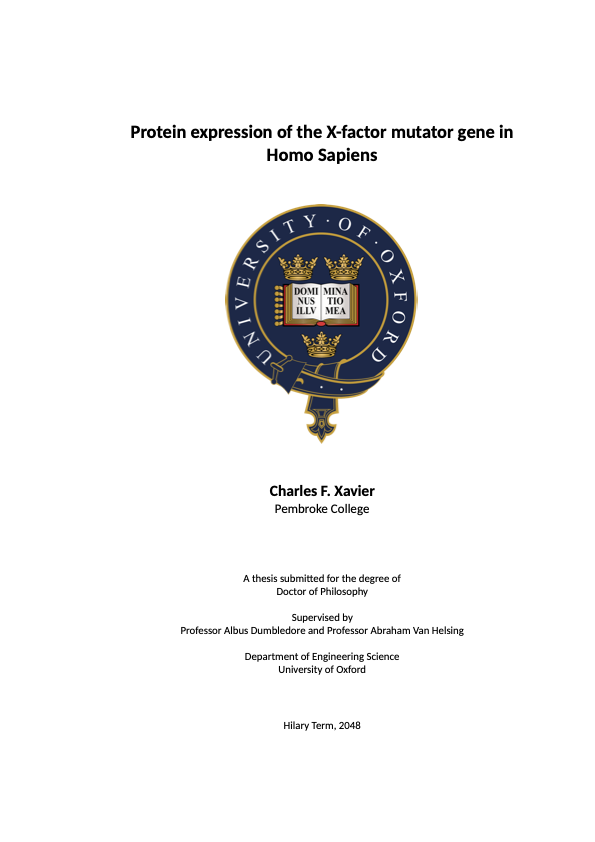
\includegraphics[width=0.45\linewidth]{dphil-title_page}
    }
    \subbottom[\label{fig:ch0:title_page:4yp}]{
        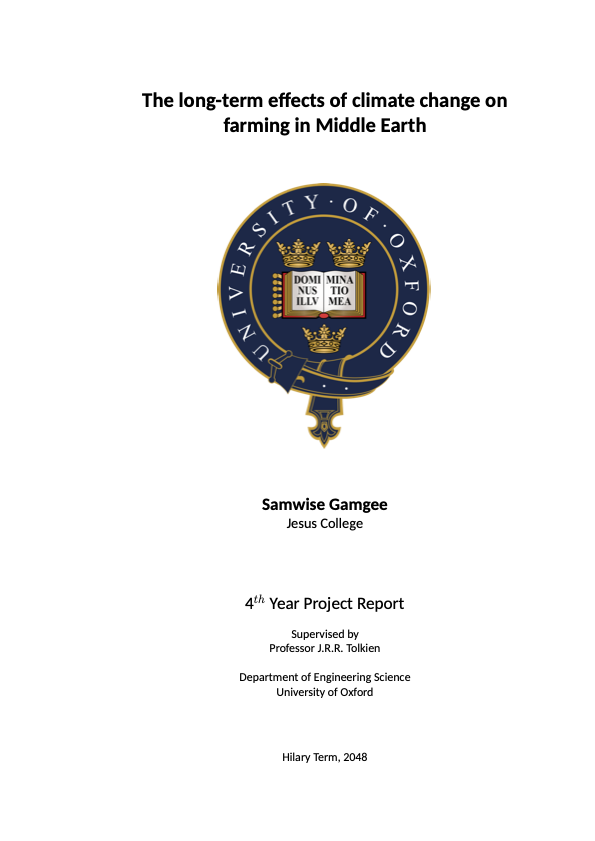
\includegraphics[width=0.45\linewidth]{4yp-title_page}
    }
    \caption[Examples of title pages for a DPhil thesis and a 4$^{th}$ Year Project report]
    {
        Examples of title pages for a \subcaptionref{fig:ch0:title_page:dphil} DPhil thesis and a
        \subcaptionref{fig:ch0:title_page:4yp} 4$^{th}$ Year Project report.
        \label{fig:ch0:title_page}
    }
\end{figure}


\Cref{fig:ch0:title_page} shows examples of the title pages for a DPhil thesis and for a 4YP report using the default title page (file``\verb|titlepage-oxford.tex|''). Both title pages were created with similar code with the ``\verb|report|'' package option as the only difference. The title page for the DPhil thesis (see \cref{fig:ch0:title_page:dphil}) was created with the following code:


\begin{lstlisting}[style=custom-latex]
\documentclass{oxengthesis}

\title{The long-term effects of climate change on farming in Middle Earth}
\author    {Samwise Gamgee}
\college   {Jesus College}
\supervisor{Professor J.R.R. Tolkien}
\date      {Hilary Term, 2048}
\end{lstlisting}


\noindent The title page for the 4YP report (see \cref{fig:ch0:title_page:4yp}) was created with the following code:


\begin{lstlisting}[style=custom-latex]
\documentclass[report]{oxengthesis}

\title{The long-term effects of climate change on farming in Middle Earth}
\author    {Samwise Gamgee}
\college   {Jesus College}
\supervisor{Professor J.R.R. Tolkien}
\date      {Hilary Term, 2048}
\end{lstlisting}


\subsection{Creating your own title page}


If you don't provide a custom title page, the OxEngThesis class will load the default title file ``\verb|titlepage-oxford.tex|'' shown above. If the layout of the default title page does not fulfil your or your university's requirements, you can create your own title page. To do so, you will need to follow the 3 steps described below. As an example, we will create a custom title page for a PhD thesis for a student at the Massachusetts Institute of Technology:

\begin{enumerate}

    \item Create a new LaTeX source file and add your own definitions, such as the example file ``\verb|titlepage-mit.tex|''

    \item Define the \verb|\titlepage{}| variable in the preamble of your ``\textit{main LaTeX source file}''. For example, after the \verb|\author{}| variable as in:


\begin{lstlisting}[style=custom-latex]
\title{Protein expression of the X-factor mutator gene in Homo Sapiens}
\author{Charles F. Xavier}
\titlepage{titlepage-mit.tex}
\end{lstlisting}


    \item Recompile your ``\textit{main LaTeX source file}''. An example of the output is shown in \cref{fig:ch0:mit_phd-title_page}


\end{enumerate}



\begin{figure}[htb]
    \centering
    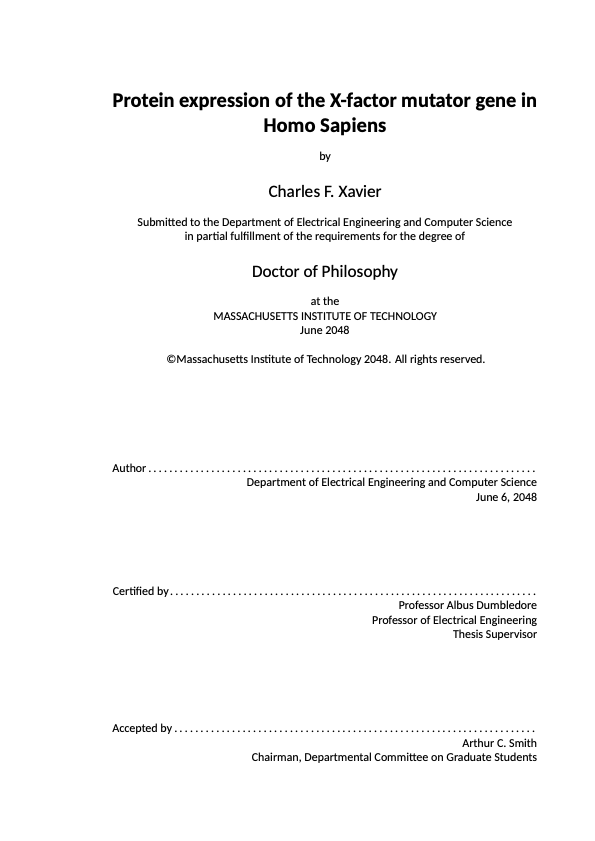
\includegraphics[width=0.7\linewidth]{mit_phd-title_page}
    \caption[Example of a title page for the Massachusetts Institute of Technology]
    {
        Example of a title page for the Massachusetts Institute of Technology.
        \label{fig:ch0:mit_phd-title_page}
    }
\end{figure}


The text below uses the \verb|titlepage-cambridge.tex| file to create a title page for a student at the University of Cambridge. The output is shown in \cref{fig:ch0:cambridge_phd-title_page}.


\begin{lstlisting}[style=custom-latex]
\title{Protein expression of the X-factor mutator gene in Homo Sapiens}
\author     {Charles F. Xavier}
\college    {Pembroke College}
\degreeprefix {A thesis submitted for the degree of}
\degree     {Doctor of Philosophy}
\supervisor {Professor Albus Dumbledore}
\department {Department of Engineering}
\university {University of Cambridge}
\universitylogo{cambridge-logo}
\date       {June 2048}
\titlepage  {titlepage-cambridge.tex}
\end{lstlisting}


\begin{figure}[htb]
    \centering
    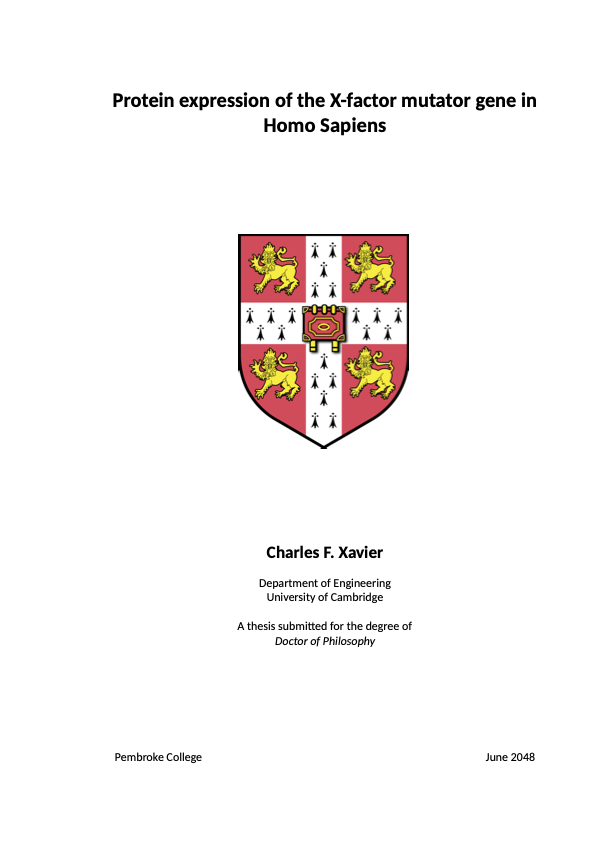
\includegraphics[width=0.7\linewidth]{cambridge_phd-title_page}
    \caption[Example of a title page for the University of Cambridge]
    {
        Example of a title page for the University of Cambridge.
        \label{fig:ch0:cambridge_phd-title_page}
    }
\end{figure}


The OxEngThesis class makes available new LaTeX commands that you can use in your new custom title document. These new commands are based on the variables defined in the preamble of your ``\textit{main LaTeX source file}'':


\begin{itemize}

    \item The \verb|\title{}| variable in the preamble will map to the command \verb|\TitleName|

    \item The \verb|\author{}| variable in the preamble will map to the command \verb|\AuthorName|

    \item The \verb|\supervisor{}| variable in the preamble will map to the command \verb|\SupervisorName|

    \item The \verb|\college{}| variable in the preamble will map to the command \verb|\CollegeName|

    \item The \verb|\degreeprefix{}| variable in the preamble will map to the command \verb|\DegreePrefix|

    \item The \verb|\degree{}| variable in the preamble will map to the command \verb|\DegreeName|

    \item The \verb|\department{}| variable in the preamble will map to the command \verb|\DepartmentName|

    \item The \verb|\university{}| variable in the preamble will map to the command \verb|\UniversityName|

    \item The \verb|\universitylogo{}| variable in the preamble will map to the command \verb|\UniversityLogo|

    \item The \verb|\date{}| variable in the preamble will map to the command \verb|\DegreeDate|

\end{itemize}


Check the files ``\verb|titlepage-oxford.tex|'', ``\verb|titlepage-mit.tex|'' and ``\verb|titlepage-cambridge.tex|'' for examples on how to use the available commands in your new title page.


\section{Package options}


\subsection{Default options}


By default, the class is formatted to produce a doctoral thesis for the University of Oxford. If you don't provide any package options in your ``\textit{main LaTeX source file}'' (as it is written in the \verb|sample_dphil_thesis.tex| file provided in this repository), such as:


\begin{lstlisting}[style=custom-latex]
\documentclass{oxengthesis}
\end{lstlisting}


\noindent the following options will be used:


\begin{lstlisting}[style=custom-latex]
\documentclass[10pt,a4paper,openany,onecolumn,twoside,final,font=Carlito,mathfont="Latin Modern Math",headingcolour={0,0,0},leftmargin=4cm,rightmargin=2cm,topmargin=2cm,bottommargin=2.5cm]{oxengthesis}
\end{lstlisting}


\noindent which will produce a thesis using a 10-point Carlito font on A4 paper size. Page margins will be formatted as required by Oxford. Chapters will start on either recto or verso pages (\verb|openany|). Note that the options ``\verb|[onecolumn,twoside,final]|'' cannot be changed.


The OxEngThesis class template is based on the \textit{memoir}\footnote{\url{https://ctan.org/pkg/memoir}} LaTeX package. As such, you can pass most of the \textit{memoir}'s option and, therefore, customise your document even further.


\subsection{Page size and margins}


By default, the page size and margins are set to comply with the requirements of the University of Oxford. Other institutions have different requirements. For example, the requirements for a thesis at the Massachusetts Institute of Technology (taken from MIT libraries\footnote{\url{https://libraries.mit.edu/distinctive-collections/thesis-specs}}) are:


\begin{lstlisting}[style=custom-text]
... For the main body of the text, including appendices and front matter, font size should be at least 11-point ...

... Top, bottom, and both side margins must be at least an inch wide (1″) to allow for binding and trimming....
\end{lstlisting}


Therefore, you would configure the class with the following options (Note that the left margin is larger to account for the thesis binding):


\begin{lstlisting}[style=custom-latex]
\documentclass[11pt,letterpaper,leftmargin=1.5in,rightmargin=1in,topmargin=1in,bottommargin=1in]{oxengthesis}
\end{lstlisting}


\subsection{Fonts}


By default, the main font is 10-point \textit{Carlito}\footnote{\url{https://ctan.org/tex-archive/fonts/carlito}} and the font for equations and formulas is ``\textit{Latin Modern Math}''\footnote{\url{https://ctan.org/tex-archive/fonts/lm-math}}. You can change to, for example, 11pt \verb|Arial| as the main font and ``\verb|tex-gyre-math-termes|'' as the font for equations with the following package options:


\begin{lstlisting}[style=custom-latex]
\documentclass[11pt,font=Arial,mathfont="TeX Gyre Termes Math"]{oxengthesis}
\end{lstlisting}


\subsection{Mini-table of contents for each chapter}


If you have a recent version of LaTeX installed (TeXLive version 2022 works) in your system and would like to have a short table of contents at the beginning of each chapter, you can simply add the ``\verb|chaptertoc|'' option to your document, as in:


\begin{lstlisting}[style=custom-latex]
\documentclass[chaptertoc]{oxengthesis}
\end{lstlisting}


\Cref{fig:ch0:dphil-chap_minitoc} shows a sample output for one chapter. I use the \textit{minitoc}\footnote{\url{https://ctan.org/pkg/memoir}} package to create the table of contents for each chapter. Previous versions of the minitoc class where incompatible with the \textit{memoir} class. I tested TexLive 2022 and MacTeX 2022, they both work fine.


\begin{figure}[htb]
    \centering
    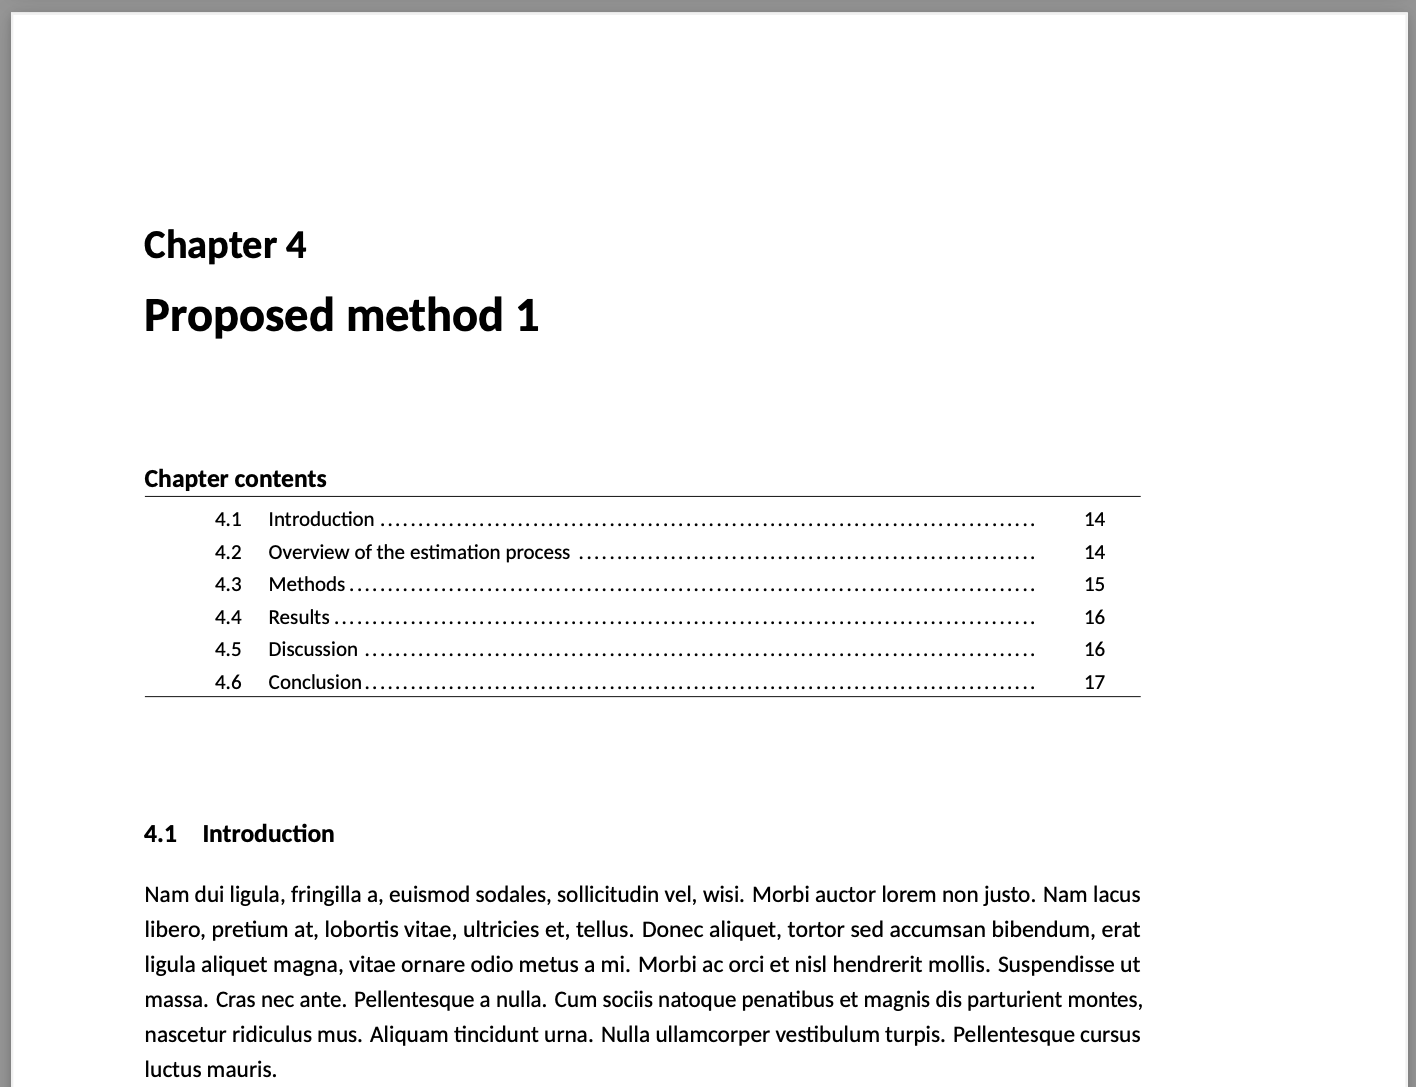
\includegraphics[width=0.7\linewidth]{dphil-chap_minitoc}
    \caption[Example of the table of contents for a chapter]
    {
        Example of the table of contents for a chapter.
        \label{fig:ch0:dphil-chap_minitoc}
    }
\end{figure}


\subsection{Abstract page for the Examination Schools}


When submitting your final thesis to the ``Examination Schools'' (located on High Street) at the University of Oxford to schedule your viva examination, you are typically required to submit two printed copies of your thesis (soft-bound). Additionally, you are required to provide two separate one-page printed copies of your abstract. The stand-alone abstract page should contain your name, college affiliation and is NOT meant to be part of the binding of your thesis. To create this single stand-alone page of your abstract, add the ``\verb|frontabstract|'' option to your document, as shown in the code below. The page will be created before the main title page, as shown in \cref{fig:ch0:dphil-front_abstract_page}.


\begin{lstlisting}[style=custom-latex]
\documentclass[frontabstract]{oxengthesis}
\end{lstlisting}


\begin{figure}[htb]
    \centering
    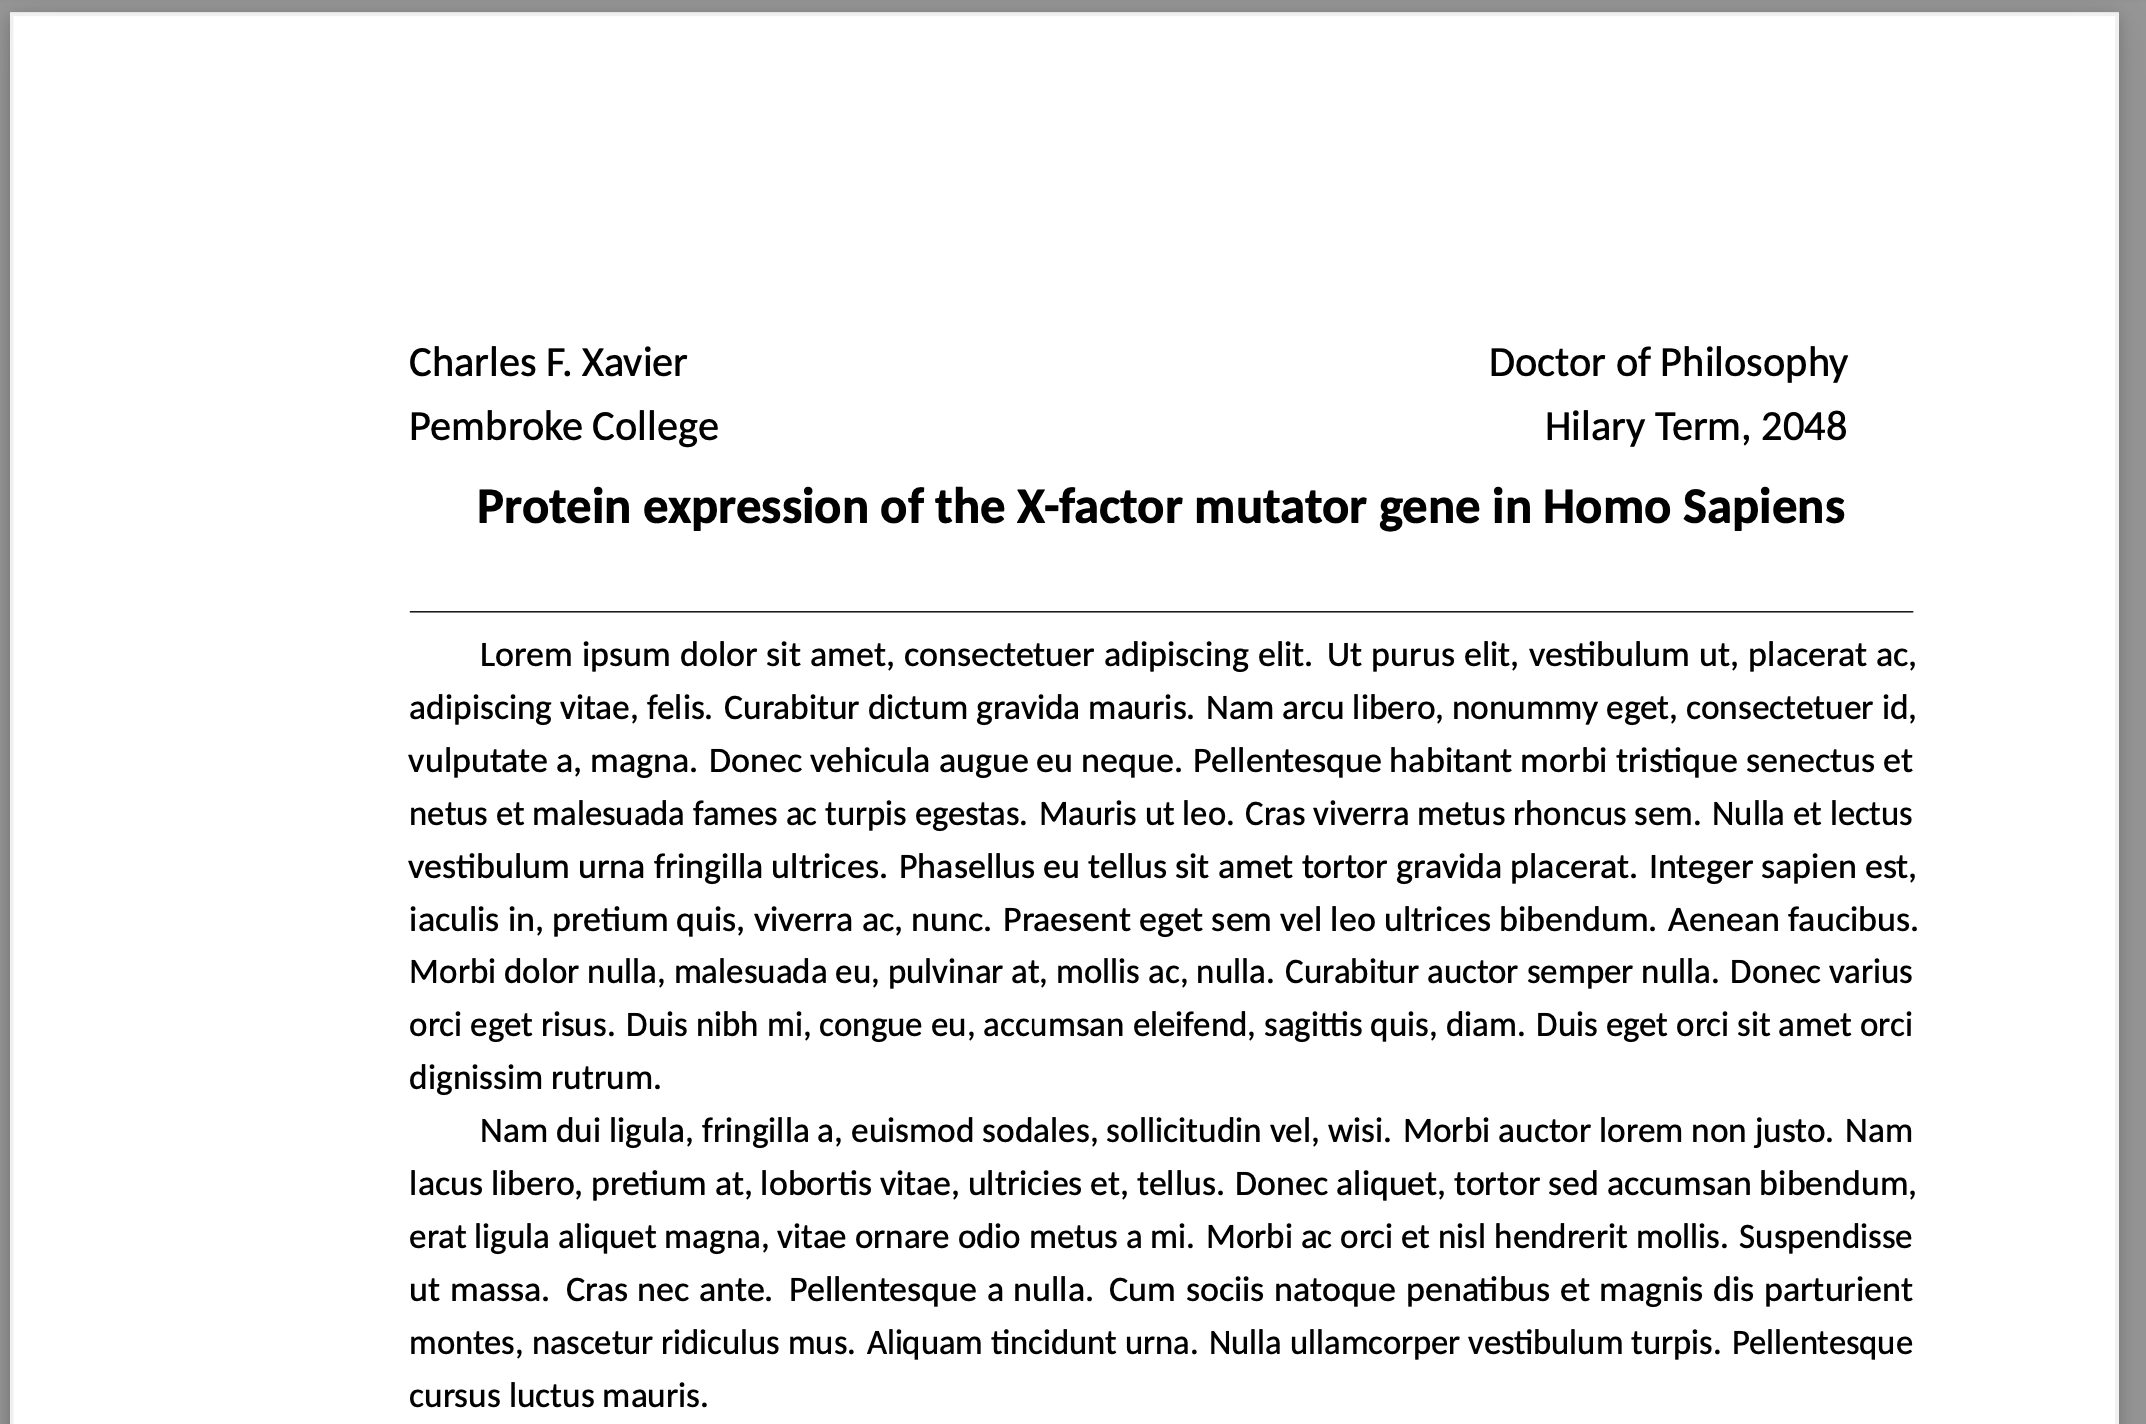
\includegraphics[width=0.7\linewidth]{dphil-front_abstract_page}
    \caption[Example of the abstract page for the Examination Schools]
    {
        Example of the abstract page for the Examination Schools.
        \label{fig:ch0:dphil-front_abstract_page}
    }
\end{figure}


\subsection{Review editing mode}


Your thesis supervisor may request you to print your document with double line spacing so he/she can correct your draft (the \textcolor{red}{red pen!}). You can simply add the ``\verb|review|'' option to your document:


\begin{lstlisting}[style=custom-latex]
\documentclass[review]{oxengthesis}
\end{lstlisting}


\subsection{Different colour for section headings}


The default font colour for section and subsection headings is black. You can change the colour (to blue for example) by adding the ``\verb|headingcolour|'' class option:


\begin{lstlisting}[style=custom-latex]
\documentclass[headingcolour={0.25,0.45,0.76}]{oxengthesis}
\end{lstlisting}


Note that the colour of \verb|\subsubsection| headings will be black regardless of the setting above.


\subsection{Chapter heading styles}


The default style for chapter headings is simple and gives you enough space to write your content. You can take advantage of different chapter styles defined in the \textit{memoir}\footnote{\url{https://ctan.org/pkg/memoir}} package by passing the ``\verb|chapterstyle|'' option. The code shown below will use the ``\verb|southall|'' chapter style to produce the sample \cref{fig:ch0:chapterstyle-southall}.


\begin{lstlisting}[style=custom-latex]
\documentclass[chapterstyle=southall]{oxengthesis}
\end{lstlisting}


\begin{figure}[htb]
    \centering
    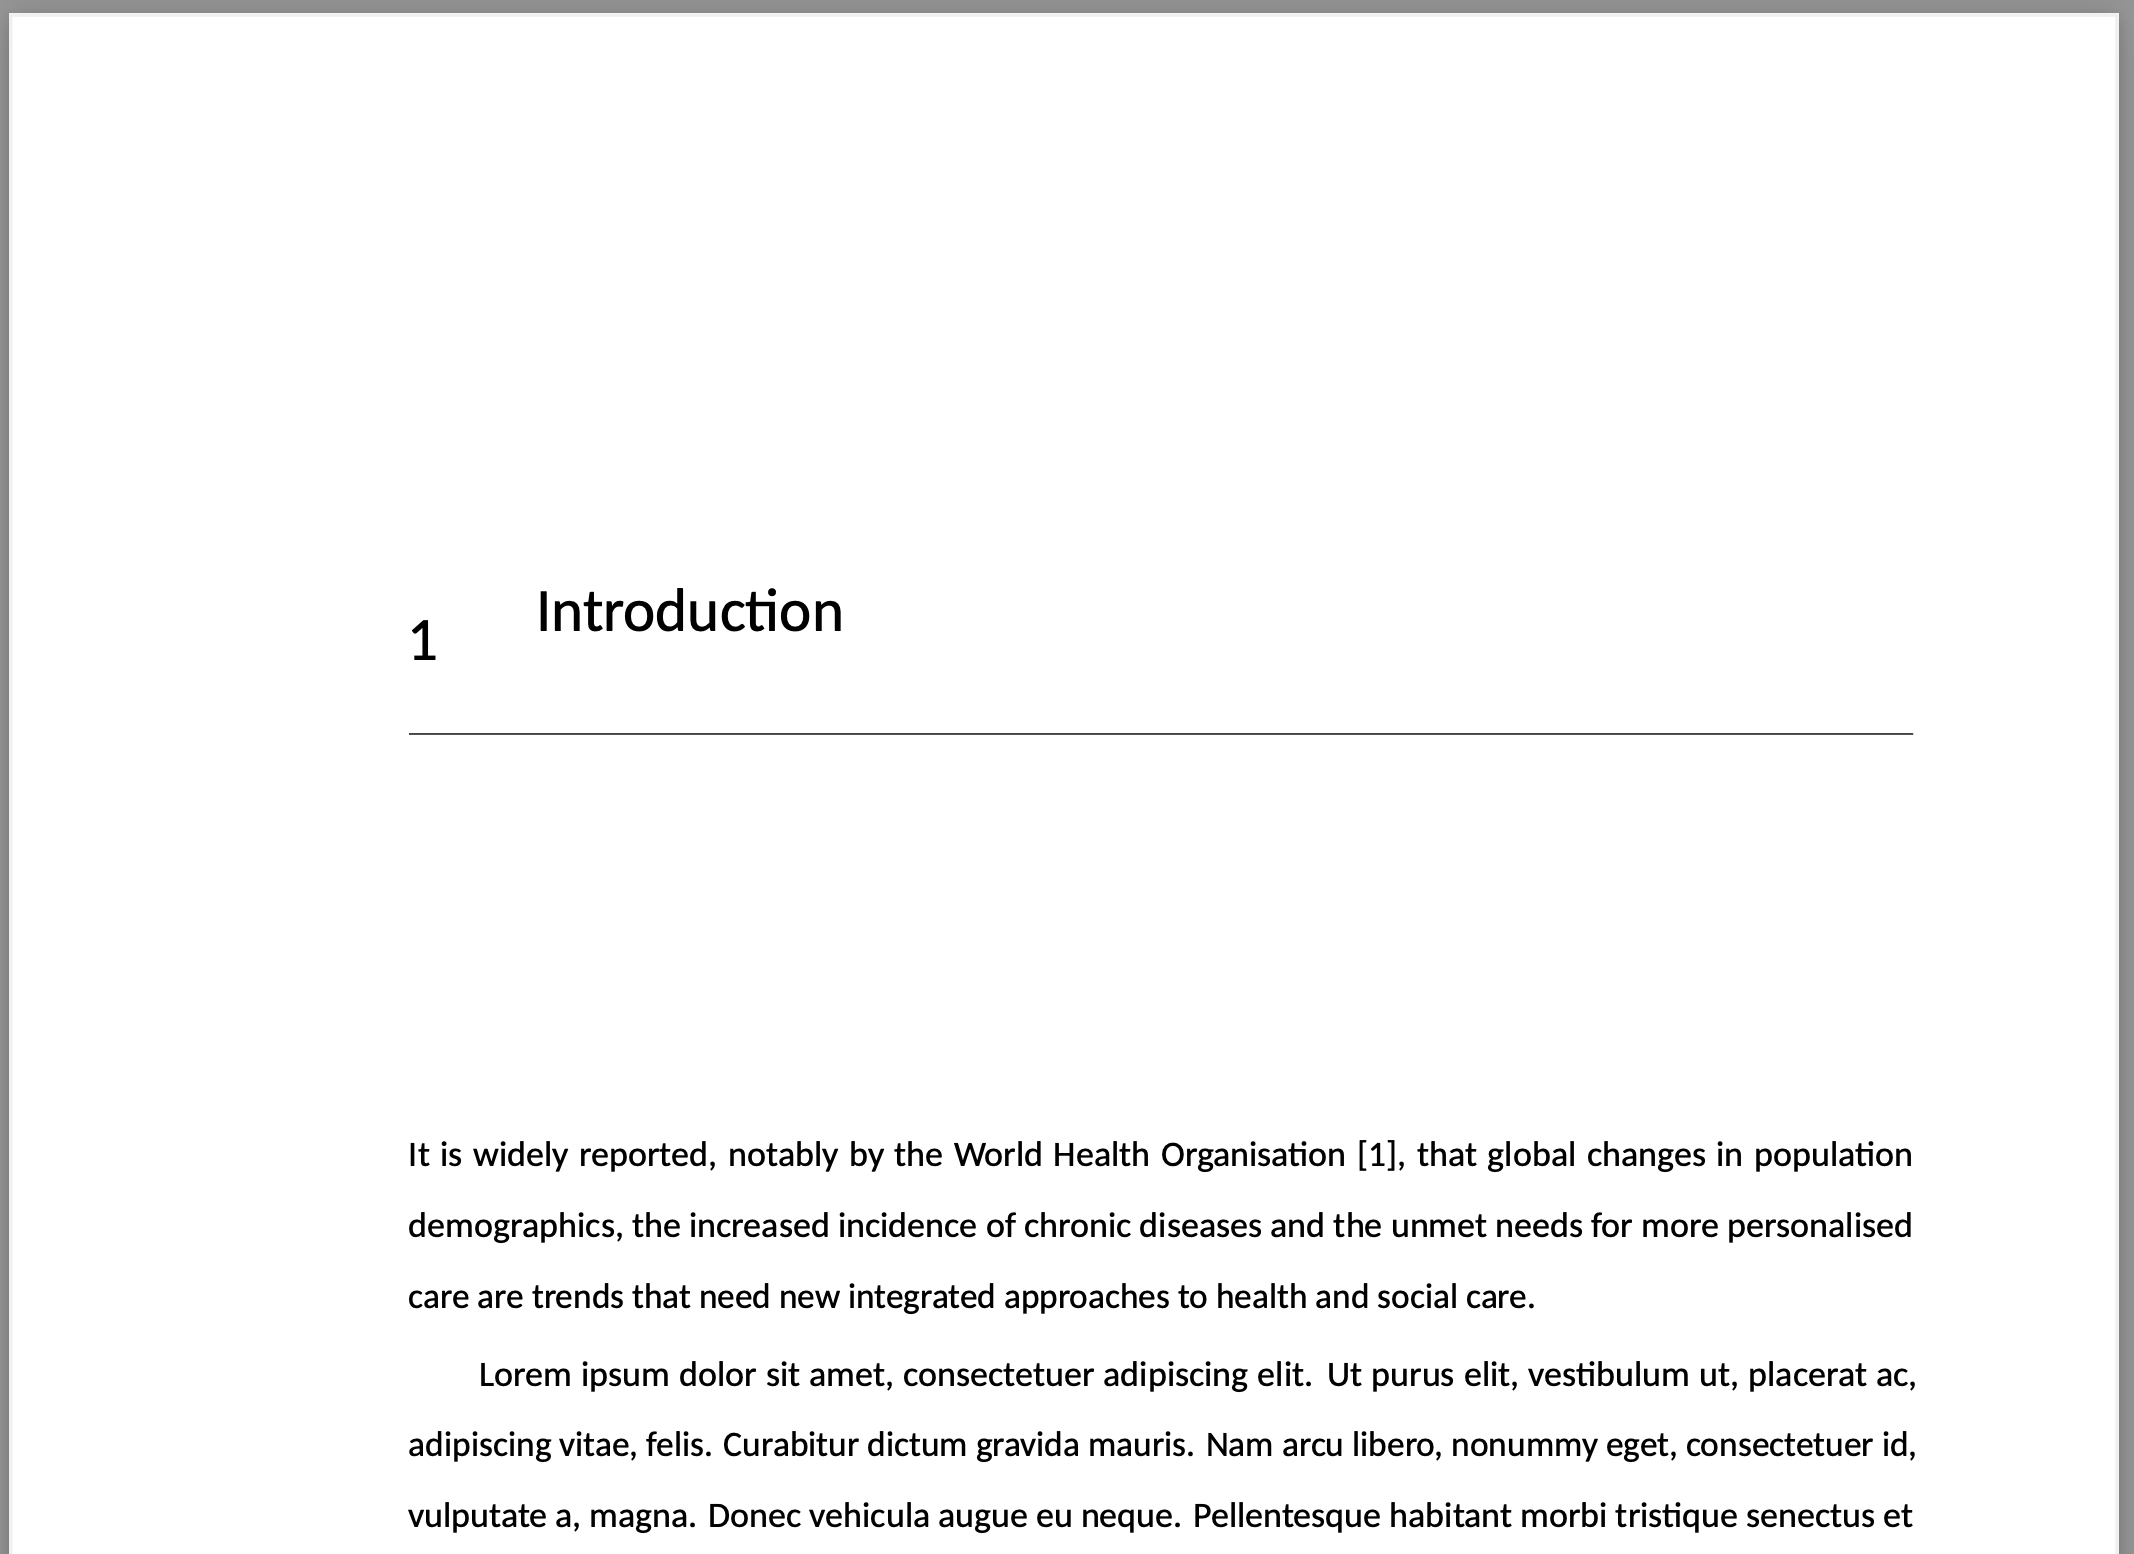
\includegraphics[width=0.7\linewidth]{chapterstyle-southall}
    \caption[The southall chapter heading style]
    {
        The southall chapter heading style.
        \label{fig:ch0:chapterstyle-southall}
    }
\end{figure}


\section{Additional features}


This section describes some of the additional features available in the OxEngThesis class. Refer to the official documentation of the \textit{memoir}\footnote{\url{https://ctan.org/pkg/memoir}} LaTeX package to customise your document even further.


\subsection{Figures}


\begin{figure}[htb]
    \centering
    \includegraphics[width=0.5\linewidth]{dummy_image}
    \caption[Sample figure covering 50\% of the page width]
    {
        Sample figure covering 50\% of the page width.
        \label{fig:ch0:sample_image}
    }
\end{figure}


I use the \textit{graphicx}\footnote{\url{https://ctan.org/pkg/graphicx}} package to include figures. You can put all figures in a ``\url{figures/}'' folder and you can simply include the image file directly without the file extension. For example, \cref{fig:ch0:sample_image} shows the image file ``\url{./figures/dummy_image.png}''. You can also create a figure with sub plots, as shown in \cref{fig:ch0:subfig_example}. Note that you can directly refer to the subplot as ``\cref{fig:ch0:subfig_example:fig1}''.


\begin{figure}
    \centering
    \subbottom[\label{fig:ch0:subfig_example:fig1}]{
        \includegraphics[width=0.3\linewidth]{dummy_image}
    }
    \subbottom[\label{fig:ch0:subfig_example:fig2}]{
        \includegraphics[width=0.3\linewidth]{dummy_image}
    }
    \subbottom[\label{fig:ch0:subfig_example:fig3}]{
        \includegraphics[width=0.3\linewidth]{dummy_image}
    }
    \caption[Sample figure with sub figures]
    {
        Sample figure with sub figures, showing:
        \subcaptionref{fig:ch0:subfig_example:fig1} caption for subfigure 1,
        \subcaptionref{fig:ch0:subfig_example:fig2} caption for subfigure 2 and
        \subcaptionref{fig:ch0:subfig_example:fig3} caption for subfigure 3.
        \label{fig:ch0:subfig_example}
    }
\end{figure}


\subsection{Tables}


\begin{table}[htb]
    \centering
    \caption{General features and specification for ...}
    \singleTableRowHeight
    \begin{tabular}{ll}

        \tableHeaderStart
        \tableHCell{Item} & \tableHCell{Description} \\
        \tableHeaderEnd

        Imaging Sensor        & Sony ICX625 2/3" progressive scan CCD \\
        Image size (pixels)   & 2448 (H) x 2048 (V)                   \\
        Pixel Size            & 3.45 \si{\micro\metre} x 3.45 \si{\micro\metre} \\
        A/D Converter         & AD9977 14-bit, dual-channel           \\
        Max frame rate        & 15 FPS                                \\
        Video Data Output     & 8, 12, 16 and 24-bit digital data     \\
        Gain \& Exposure                  & Automatic/Manual/One-Push \\
        Lens Mount            & C-mount                               \\
        Interface             & Gigabit Ethernet                      \\
        Physical dimensions   & 44 (W) mm x 29 (H) mm x 58 (L) mm     \\
        \hline 

    \end{tabular}
    \label{table:ch0:camera_specs}
\end{table}


You can create tables using the regular syntax in LaTeX. You can also create tables with additional styles. For example, \cref{table:ch0:camera_specs} shows a classical table with shaded headers. You can have more complex tables, as shown in \cref{table:ch0:patient_demographics}


\begin{table}[htb]
  \centering
  \caption{Summary of population demographics in the training and test sets}
  {
    \small
    \begin{tabular}{p{2cm} c c c c c c c c c c}
      \toprule

      Set &
      \multirowcell{2}{Number of\\subjects} &
      \multirowcell{2}{Total time\\(hours)}$^1$ &
      \multicolumn{2}{c}{Gender} &      
      \multicolumn{6}{c}{Ethnicity$^2$}  \\

      \cmidrule{4-11}
        
      &  &  & Male & Female & W & B & A & WB & WA & O  \\
      \midrule
      Training  & 15 & 216.6 & 8  & 7  & 10 & 1   & 1 & 1 & 1 & 1 \\        
      Test      & 15 & 210.0 & 10 & 5  & 10 & $-$ & 1 & 1 & 2 & 1 \\        
      \midrule        
      Total	& 30 & 426.6 & 18 & 12 & 20 & 1   & 2 & 2 & 3 & 2 \\
        
      \bottomrule
        
      \multicolumn{11}{l}
      {
        \footnotesize $^1$ Period during which both reference and estimated data were being recorded simultaneously.        
      } \\        
      \multicolumn{11}{l}
      {        
        \footnotesize $^2$ W = White, B = Black, A = Asian, WB = Mixed White \& Black, WA = Mixed White \& Asian and O = Other.        
      } \\
        
      \end{tabular}      
  } 
  \label{table:ch0:patient_demographics}
\end{table}


\subsection{Cross-referencing labels}


I use the \textit{cleveref}\footnote{\url{https://ctan.org/pkg/cleveref}} package to automatically format the label when cross referencing chapters, sections, figures and other common LaTeX labels. The following paragraphs, show some of the results.

You don't have to include the word ``chapter'': \Cref{chapter:literature_review} discusses .... is presented in \cref{chapter:dataset} with a detailed ...

You don't have to include the word ``figure'' or ``table'': The summary of the demographics for the entire set is described in \cref{table:ch0:patient_demographics} ... \Cref{fig:ch0:subfig_example} shows the video camera used in the study. \Cref{fig:ch0:subfig_example:fig1} shows the the camera model used, \cref{fig:ch0:subfig_example:fig2} shows the ... and \cref{fig:ch0:subfig_example:fig3} shows...


\subsection{Glossary, acronyms and abbreviations}


I use the \textit{glossaries-extra}\footnote{\url{https://ctan.org/pkg/glossaries-extra}} packages to define acronyms and automatically add the ``Glossary'' page in the \textit{frontmatter}. Simply create a file with the name ``glossary.tex'' and add all your definitions to it. Note that the first time you use an acronym, its full definition will be provided. For the rest of the instances, only the abbreviation will be used. The following paragraphs show how to define and use acronyms.

The standard vital signs include temperature, \ab{hr}, \ab{rr}, \ab{bp} and, when appropriate, \ab{spo2}. The routine measurement and interpretation of these vital signs is a core component of the physiological assessment of most patients \cite{prior1977physical,goldberg2005practical} as they can provide critical information about the underlying state of their health. 

We included all study types looking at monitoring of \ab{hr}, \ab{bp}, \ab{rr} or \ab{spo2} using image analysis with comparison to a reference device. We did not restrict based on clinical setting and included all age groups. Only non-contact methods using cameras were included. All unpublished studies found were included wherever possible to minimise publication bias.


\subsection{Citations and references}


This section contains example on how to cite papers, journals and other documents:

It is widely reported, notably by the World Health Organisation \cite{stroetmann2010can}, that global changes in population demographics, the increased incidence of chronic diseases and the unmet needs for more personalised care are trends that need new integrated approaches to health and social care. \cite{brooks1984infrared}


\lipsum[1]\cite{barker1987pulse,peacock1998oxygen,moller1993randomized}


Finding reliable correspondences in two images of a scene taken from arbitrary viewpoints viewed with possibly different cameras and in different illumination conditions is a difficult and critical step towards fully automatic reconstruction of 3D scenes\cite{hartley2003multiple}.


\lipsum[7]\cite{priya2012transition,haralick1973textural,Grass2012Online,NoninPulseOxOnline}


\subsection{Bibliography styles}


The default style for the references is ``\verb|ieeetr|''. For example, the following text: ``\textit{...Finding reliable correspondences in two images of a scene taken from arbitrary viewpoints viewed with possibly different cameras and in different illumination conditions is a difficult and critical step towards fully automatic reconstruction of 3D scenes \cite{hartley2003multiple}...}'' will produce the following output in the bibliography section at the end of the thesis:


\begin{lstlisting}[style=custom-text]
Bibliography
...
[8] R. Hartley and A. Zisserman, Multiple view geometry in computer vision. Cambridge university press, 2003.
...
\end{lstlisting}


You can specify a custom bibliography style as an argument to the ``\verb|\listofreferences|'' command in your \textit{main LaTeX source file}. For example, the following command:


\begin{lstlisting}[style=custom-latex]
\listofreferences[apalike]
\end{lstlisting}


\noindent will use the \textit{apalike}\footnote{\url{https://www.bibtex.com/s/bibliography-style-base-apalike}}
BibTeX style and produce the following output in the content pages:


\begin{lstlisting}[style=custom-text]
...Finding reliable correspondences in two images of a scene taken from arbitrary viewpoints viewed with possibly different cameras and in different illumination conditions is a difficult and critical step towards fully automatic reconstruction of 3D scenes [Hartley and Zisserman, 2003]...
\end{lstlisting}


\noindent and the bibliography section will read:


\begin{lstlisting}[style=custom-text]
Bibliography
...
[Hartley and Zisserman, 2003] Hartley, R. and Zisserman, A. (2003). Multiple view geometry in computer vision. Cambridge university press.
...
\end{lstlisting}

Take a look at the available styles at \textit{The quick BibTeX guide}\footnote{\url{https://www.bibtex.com/styles}} online.


\subsection{Mark text as TODO}


You can wrap text in``todo'' tags, so they appear in red colour in the PDF document. For example:

\todo{This text is in red colour, it reminds me of a task to complete}


\subsection{Formatting source code}


Often, we want to show pseudo code, source code or other verbatim content in our document. For this, I use the \textit{listings}\footnote{\url{https://ctan.org/pkg/listings}} package. The extra custom styles defined in the OxEngThesis class file are:


Example on displaying C/C++ source code:


\begin{lstlisting}[style=custom-c,caption={Function to balance a matrix.}]
extern PE_SIGPROC_API void pesig_balance(
        const size_t    n,
        signal_value_t  A[n][n],
        signal_value_t* S
        );
\end{lstlisting}


Example on displaying BASH/Console scripts:


\begin{lstlisting}[style=custom-bash,caption={A script in bash.}]
$ mkdir -p $HOME/code/pebase/realtime
$ cd $HOME/code/pebase/realtime
$ git clone git@github.com:maurovm/thesis_template.git repository
\end{lstlisting}


Example of displaying text as ``verbatim'' mode:


\begin{lstlisting}[style=custom-verbatim,caption={License information.}]
OxEngThesis is provided under:

    SPDX-License-Identifier:    GPL-2.0-only
    
OxEngThesis is free software: you can redistribute it or modify
it under the terms of the GNU General Public License as published by the
Free Software Foundation, version 2 only, according with:

    LICENSES/GPL-2.0

OxEngThesis is distributed in the hope that it will be useful, but
WITHOUT ANY WARRANTY; without even the implied warranty of MERCHANTABILITY
or FITNESS FOR A PARTICULAR PURPOSE. See the GNU General Public License
for more details.
\end{lstlisting}


\subsection{Coloured boxes}


I use the \textit{tcolorbox}\footnote{\url{https://ctan.org/pkg/tcolorbox}} package to show coloured and framed text boxes with an optional heading line. Some examples include:

\noindent Standard box:


\begin{tcolorbox}
\lipsum[1]
\end{tcolorbox}


\noindent Standard box with title:


\begin{tcolorbox}[title=Box title]
\lipsum[1]
\end{tcolorbox}


\noindent A small box following text:\dotfill\tcbox[nobeforeafter,colframe=blue!50!black,colback=white,colupper=red!50!black]{Hello World}\hfill


Read the documentation of the \verb|tcolorbox| package to see an extensive description of the configuration options and what you can do with the \verb|tcolorbox| class, it is quite customisable. The OxEngThesis class defines some environment commands for some predefined boxes. For example, the following is a warning box:


\begin{OxWarningBox}{Warning box title}
Warning box content: \lipsum[1]
\end{OxWarningBox}


The following example shows an information box:


\begin{OxInfoBox}{Informational box title}
Warning box content: \lipsum[1]
\end{OxInfoBox}


\section{Troubleshooting common errors}


\subsection{Text beyond page limits}


When compiling a LaTeX document, you could get a warning similar to:


\begin{lstlisting}[style=custom-text]
Overfull \hbox (22.49216pt too wide) in paragraph at lines 4--5
\end{lstlisting}


This often occurs when a line of your document could not fit within the designated horizontal space for text in the current page layout. The LaTeX compiler tries its best to fit text within the page limits, but sometimes it just cannot do it appropriately. This typically results in some text hanging out past the page margin due to long words, acronyms or long equations. Sometimes, it is difficult to know where these errors occur in your document. You can add the ``\verb|debuglayout|'' option to your document:


\begin{lstlisting}[style=custom-latex]
\documentclass[debuglayout]{oxengthesis}
\end{lstlisting}


\begin{figure}[htb]
    \centering
    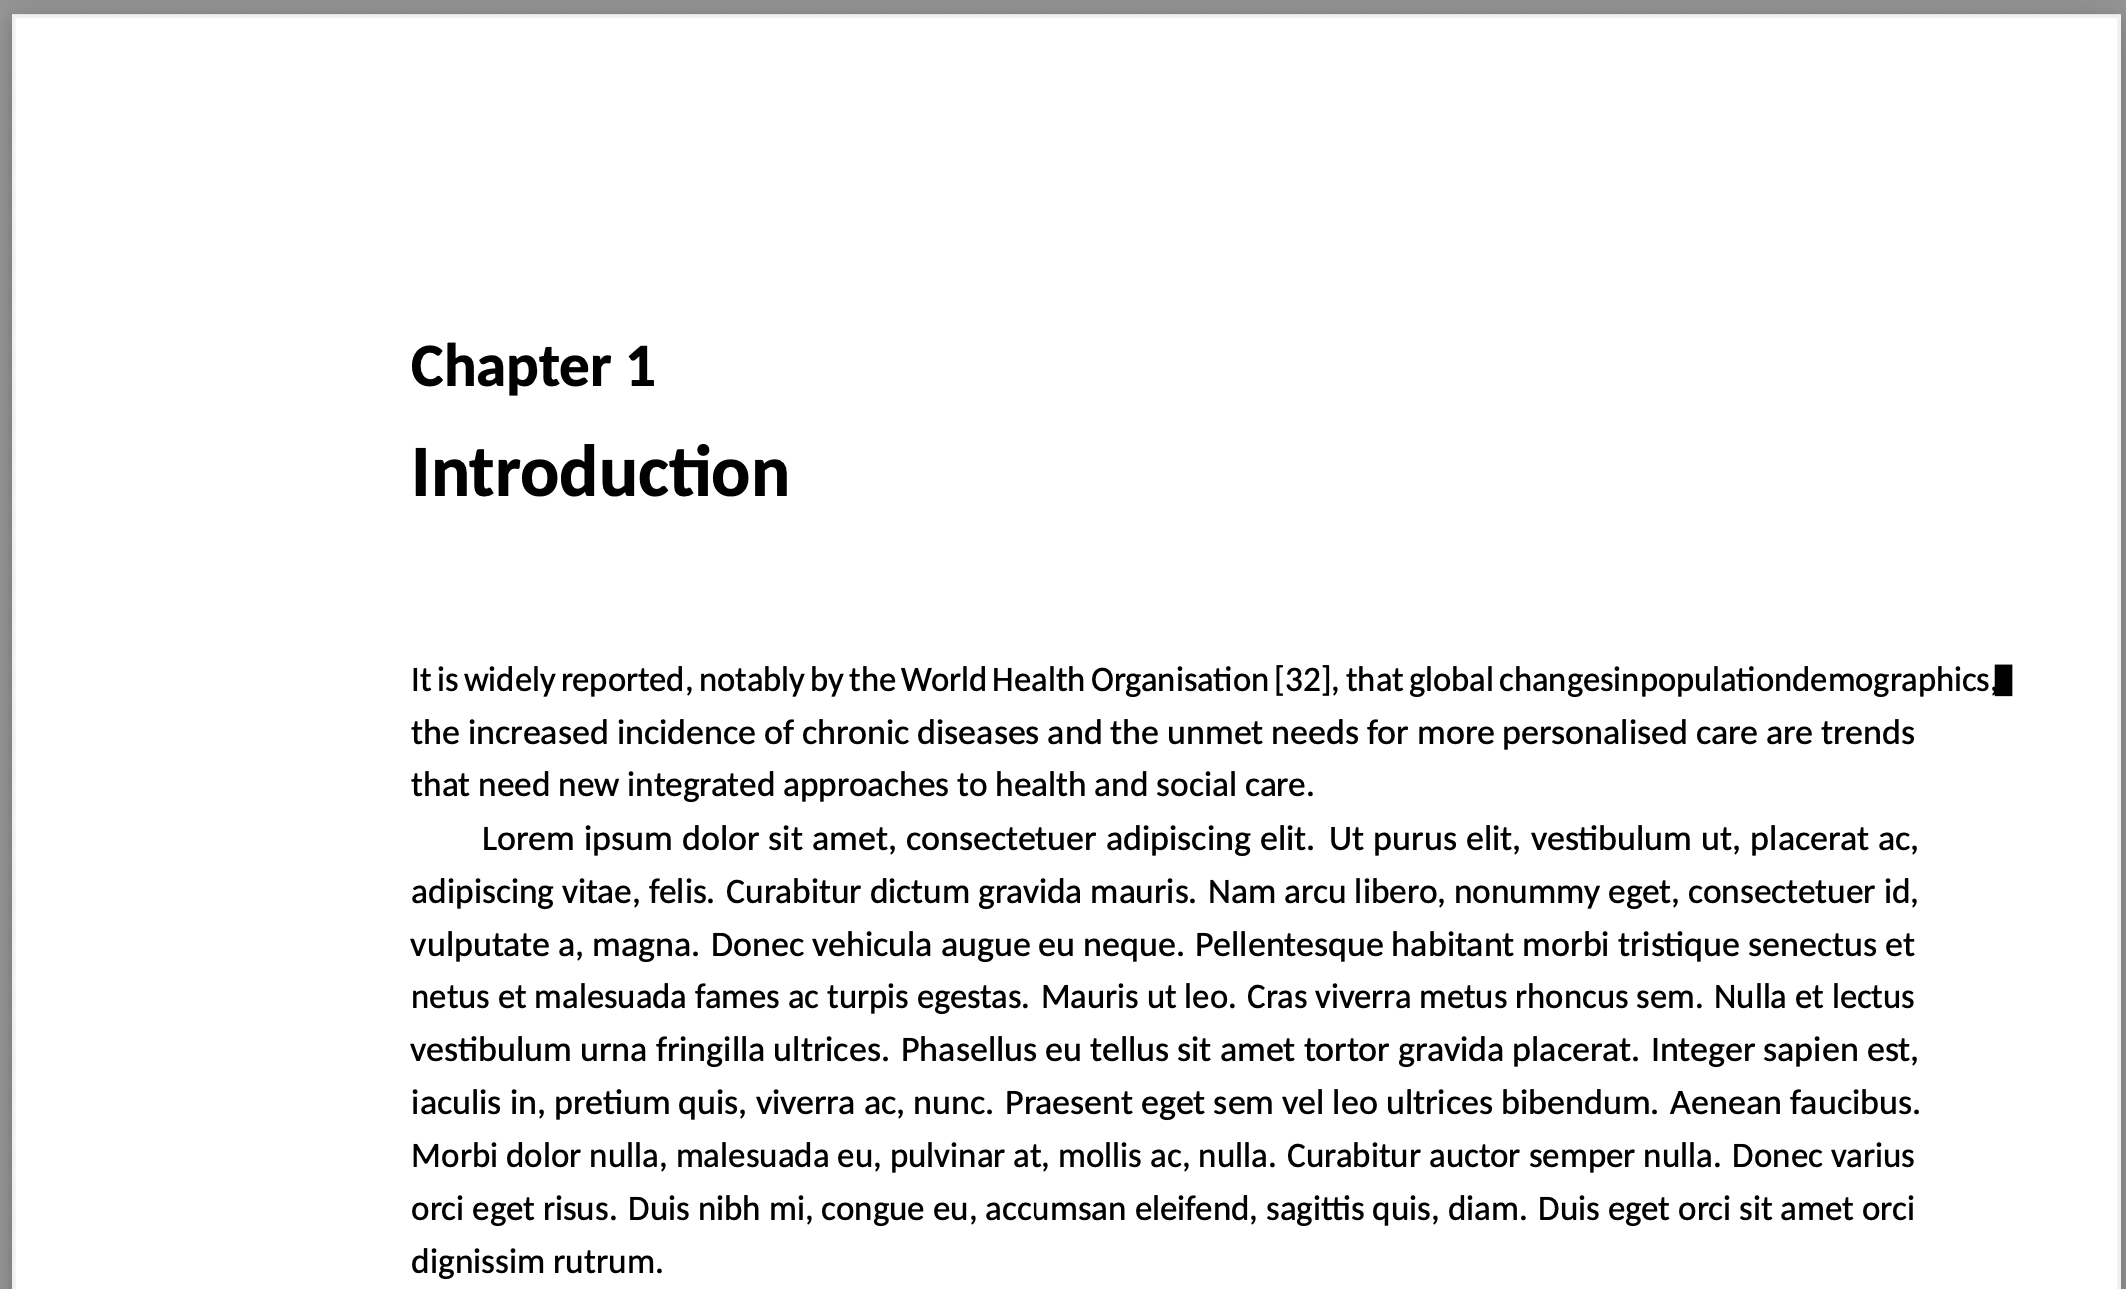
\includegraphics[width=0.7\linewidth]{overfull_hbox_warning}
    \caption[Example of a line of text that does not fit within the horizontal space for text]
    {
        Example of a line of text that does not fit within the horizontal space for text. A black box is shown next to the affected line.
        \label{fig:ch0:overfull_hbox_warning}
    }
\end{figure}


A black box will be shown next to the affected lines, as shown in \cref{fig:ch0:overfull_hbox_warning}. The \url{oxengthesis.cls} class file already takes advantage of other packages (such as \textit{microtype}\footnote{https://ctan.org/pkg/microtype}) to deal with common issues such as character protrusion, font expansion and inter-word spacing. I recommend you slightly rephrase your guilty sentences instead of changing the class template. This is usually the first approach many of my students take.


\end{lstlisting}


Note that the line above includes the chapter you are currently reading. It is only meant to showcase the features provided by the OxEngThesis class. It is numbered as ``Chapter 0'' so not to change the flow of the rest of the document.

The \textit{frontmatter} of the thesis will be automatically created depending on the type of document you are writing, either a doctoral thesis or a project report. If you want more control, you can review how the \verb|\makefrontmatterpages| command is defined in the \verb|oxengthesis.cls| class file. If you want all the sections in the \textit{frontmatter} to appear, you will need to create the following files:


\begin{itemize}
    \item \verb|abstract.tex|: If you want the ``Abstract'' page
    \item \verb|dedication.tex|: If you want the ``Dedication'' page
    \item \verb|declaration.tex|: If you want the ``Declaration'' page
    \item \verb|acknowledgements.tex|: If you want the ``Acknowledgements'' page
    \item \verb|publications.tex|: If you want the ``List of publications'' page
    \item \verb|glossary.tex|: If you want the ``List of abbreviations'' page
\end{itemize}


If any of the files above is missing, that particular page won't be created in the \textit{frontmatter}. This is useful if you are just preparing a draft version of your thesis for your supervisor to correct. 

Similarly for the \textit{backmatter} part of your thesis, add all the BibTeX citations to a file named \verb|references.bib| if you want the ``Bibliography'' section to be created at the end of your document. 


\subsection{Writing a ``Transfer of Status'' or ``Confirmation of Status'' report}


There are two Key milestones\footnote{\url{https://www.ox.ac.uk/students/academic/guidance/graduate/research/status/DPhil}} for which DPhil students are expected to submit substantial piece of written research work, or reports. They are the ``Transfer of Status''\footnote{\url{https://www.mpls.ox.ac.uk/graduate-school/information-and-resources-for-supervisors/transfer-of-status}} at the end of your first year, and the ``Confirmation of Status''\footnote{\url{https://www.mpls.ox.ac.uk/graduate-school/information-and-resources-for-supervisors/confirmation-of-status}} at the end of your second year. 

For these milestones, you will often be required to submit a report with all the details of your research contributions. This document is often around 50-60 pages in length and does not need all the sections that a doctoral thesis has (i.e. declaration, dedication or list of publications). 

You can write a \textit{Transfer of Status} report by simply providing the ``\verb|report|'' option when you load the \verb|OxEngThesis| class, and defining the ``\verb|degree|'' variable as shown in the following code snippet:


\begin{lstlisting}[style=custom-latex]
\documentclass[report]{oxengthesis}

\title       {The title of your report}
\author      {Your name}
\degree      {{\huge Transfer of Status Report}}
\college     {The name of your college}
\supervisor  {The name(s) of your supervisor(s)}
\date        {The academic term of submission}
\end{lstlisting}


You can write a \textit{Confirmation of Status} report by simply providing the ``\verb|report|'' option when you load the \verb|OxEngThesis| class, and defining the ``\verb|degree|'' variable as shown in the following code snippet:


\begin{lstlisting}[style=custom-latex]
\documentclass[report]{oxengthesis}

\title       {The title of your report}
\author      {Your name}
\degree      {{\huge Confirmation of Status Report}}
\college     {The name of your college}
\supervisor  {The name(s) of your supervisor(s)}
\date        {The academic term of submission}
\end{lstlisting}


Note that the "*report*" package option is just a shortcut to not include the dedication, declaration and publications pages and format the title page accordingly.


\subsection{Writing a 4$^{th}$-Year Project (4YP) report}


If you are an undergraduate student at the University of Oxford reading Engineering Science\footnote{\url{https://eng.ox.ac.uk/study/undergraduate/your-degree}}, you will carry out a self-led project during your fourth year. It usually involves original research or significant design and construction work, undertaken in close consultation with an academic supervisor. At the end of your project (usually by the beginning of Trinity term), you will need to submit a report with all the details of your research contributions. This document is often about 50 pages in length and does not need all the sections that a doctoral thesis has (i.e. declaration, dedication or list of publications). 

You can write a 4YP report by simply providing the ``\verb|report|'' option when you load the \verb|OxEngThesis| class, and defining the ``\verb|degree|'' variable as shown in  the following code snippet:


\begin{lstlisting}[style=custom-latex]
\documentclass[report]{oxengthesis}

\title       {The title of your report}
\author      {Your name}
\degree      {{\huge 4$^{th}$ Year Project Report}}
\college     {The name of your college}
\supervisor  {The name(s) of your supervisor(s)}
\date        {The academic term of submission}
\end{lstlisting}


\subsection{Creating the PDF output}


The source files in this repository require the LuaLaTeX engine. You editor should allow you to configure LuaLaTeX as the typesetting engine for your document and automatically take care of the compilation process to generate the final PDF document from your ``\textit{main LaTeX source file}''.

If you want to compile your ``\textit{main LaTeX source file}'' from the command line, you can use the ``\verb|compile_document.sh|'' script provided in this repository. This script only works in a Linux or macOS system. For example, to compile the sample thesis provided, you will execute the following command in the terminal:


\begin{lstlisting}[style=custom-bash]
$ ./compile_document.sh  sample_dphil_thesis.tex
\end{lstlisting}


If you want to delete all the temp or auxiliary files LaTeX created during the compilation process, you can run:


\begin{lstlisting}[style=custom-bash]
$ ./remove_latex_aux_files.sh
\end{lstlisting}


If you are compiling the document manually, you would need to run the \textit{latexmk}\footnote{\url{https://ctan.org/pkg/latexmk}} build command (already part of your LaTeX distribution) in the following order:


\begin{lstlisting}[style=custom-bash]
$ latexmk -pdflatex=lualatex -pdf  sample_dphil_thesis.tex
$ makeglossaries sample_dphil_thesis.tex
$ latexmk -pdflatex=lualatex -pdf  sample_dphil_thesis.tex
\end{lstlisting}


\subsection{Customising the title page}


Although I originally wrote this LaTeX template for a student at the University of Oxford, it should be easy for you to customise it to suit the requirements of your academic institution. The default title page ``\verb|titlepage-oxford.tex|'' is simple and customisable. The class template defines some variables you can use. At minimum, you need to provide the following definitions in the preamble of your ``\textit{main LaTeX source file}'':


\begin{itemize}

    \item \verb|\title{}|: The main title of the thesis/report
    \item \verb|\author{}|: The author of the thesis/report

\end{itemize}

You can define the following optional variables:

\begin{itemize}

    \item \verb|\supervisor{}|: The name of your thesis supervisor. The default value is: ``SUPERVISOR NAME''

    \item \verb|\college{}|: Your college affiliation, if you are an Oxford student. The default value is: ``'' (an \textit{empty string})

    \item \verb|\degreeprefix{}|: Text printed before the degree name. The default value is: ``A thesis submitted for the degree of''

    \item \verb|\degree{}|: The name of the degree. The default value is: ``Doctor of Philosophy''

    \item \verb|\department{}|: Your university department. The default value is: ``Department of Engineering Science''

    \item \verb|\university{}|: The name of your university. The default value is: ``University of Oxford''

    \item \verb|\universitylogo{}|: File name of the university's logo, without the file extension. The default value is: ``oxford-logo'' (which will load the image file \verb|oxford-logo.png| in the \verb|./figures/| folder in this repository

    \item \verb|\date{}|: The date of publication of the thesis, such as ``Hilary Term, 2048''. If you leave it blank, it will print the current date (useful when sending a draft to your supervisor)

\end{itemize}



\begin{figure}[htb]
    \centering
    \subbottom[\label{fig:ch0:title_page:dphil}]{
        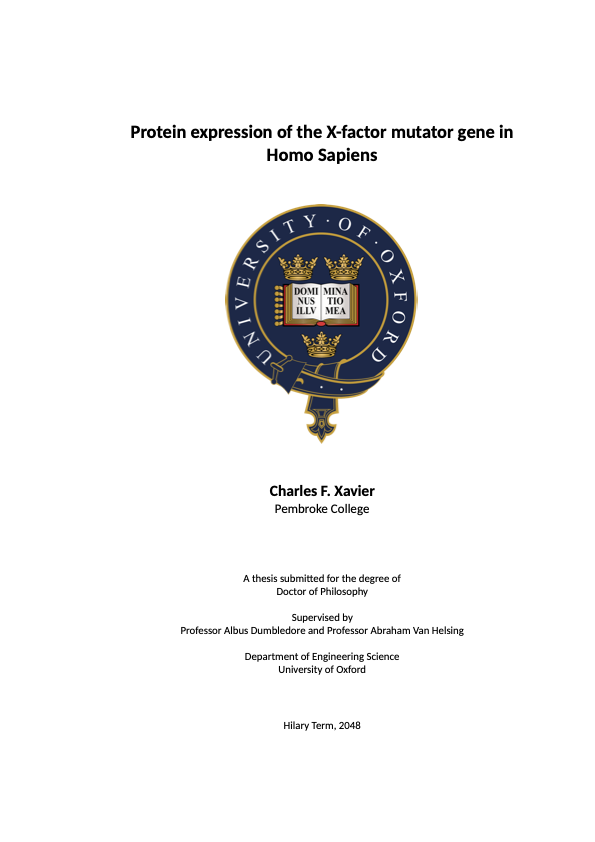
\includegraphics[width=0.45\linewidth]{dphil-title_page}
    }
    \subbottom[\label{fig:ch0:title_page:4yp}]{
        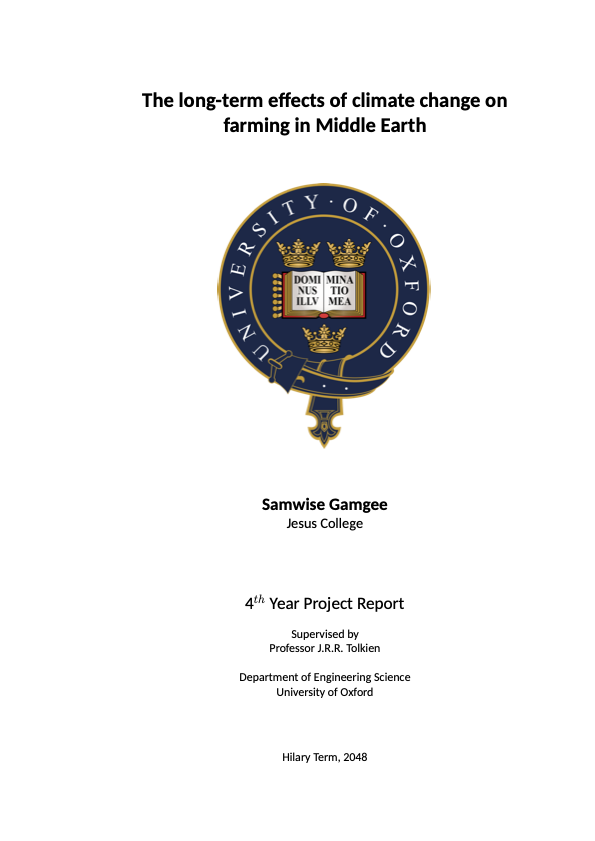
\includegraphics[width=0.45\linewidth]{4yp-title_page}
    }
    \caption[Examples of title pages for a DPhil thesis and a 4$^{th}$ Year Project report]
    {
        Examples of title pages for a \subcaptionref{fig:ch0:title_page:dphil} DPhil thesis and a
        \subcaptionref{fig:ch0:title_page:4yp} 4$^{th}$ Year Project report.
        \label{fig:ch0:title_page}
    }
\end{figure}


\Cref{fig:ch0:title_page} shows examples of the title pages for a DPhil thesis and for a 4YP report using the default title page (file``\verb|titlepage-oxford.tex|''). Both title pages were created with similar code with the ``\verb|report|'' package option as the only difference. The title page for the DPhil thesis (see \cref{fig:ch0:title_page:dphil}) was created with the following code:


\begin{lstlisting}[style=custom-latex]
\documentclass{oxengthesis}

\title{The long-term effects of climate change on farming in Middle Earth}
\author    {Samwise Gamgee}
\college   {Jesus College}
\supervisor{Professor J.R.R. Tolkien}
\date      {Hilary Term, 2048}
\end{lstlisting}


\noindent The title page for the 4YP report (see \cref{fig:ch0:title_page:4yp}) was created with the following code:


\begin{lstlisting}[style=custom-latex]
\documentclass[report]{oxengthesis}

\title{The long-term effects of climate change on farming in Middle Earth}
\author    {Samwise Gamgee}
\college   {Jesus College}
\supervisor{Professor J.R.R. Tolkien}
\date      {Hilary Term, 2048}
\end{lstlisting}


\subsection{Creating your own title page}


If you don't provide a custom title page, the OxEngThesis class will load the default title file ``\verb|titlepage-oxford.tex|'' shown above. If the layout of the default title page does not fulfil your or your university's requirements, you can create your own title page. To do so, you will need to follow the 3 steps described below. As an example, we will create a custom title page for a PhD thesis for a student at the Massachusetts Institute of Technology:

\begin{enumerate}

    \item Create a new LaTeX source file and add your own definitions, such as the example file ``\verb|titlepage-mit.tex|''

    \item Define the \verb|\titlepage{}| variable in the preamble of your ``\textit{main LaTeX source file}''. For example, after the \verb|\author{}| variable as in:


\begin{lstlisting}[style=custom-latex]
\title{Protein expression of the X-factor mutator gene in Homo Sapiens}
\author{Charles F. Xavier}
\titlepage{titlepage-mit.tex}
\end{lstlisting}


    \item Recompile your ``\textit{main LaTeX source file}''. An example of the output is shown in \cref{fig:ch0:mit_phd-title_page}


\end{enumerate}



\begin{figure}[htb]
    \centering
    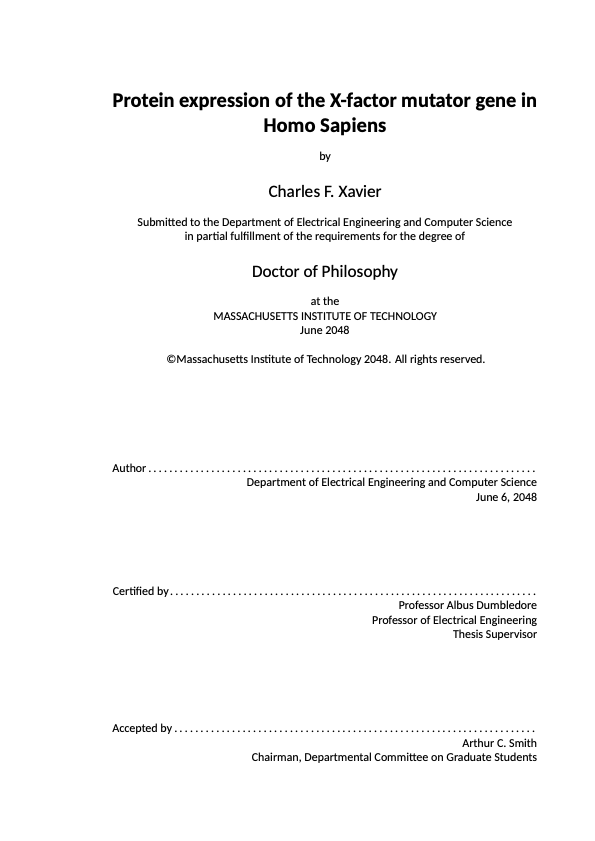
\includegraphics[width=0.7\linewidth]{mit_phd-title_page}
    \caption[Example of a title page for the Massachusetts Institute of Technology]
    {
        Example of a title page for the Massachusetts Institute of Technology.
        \label{fig:ch0:mit_phd-title_page}
    }
\end{figure}


The text below uses the \verb|titlepage-cambridge.tex| file to create a title page for a student at the University of Cambridge. The output is shown in \cref{fig:ch0:cambridge_phd-title_page}.


\begin{lstlisting}[style=custom-latex]
\title{Protein expression of the X-factor mutator gene in Homo Sapiens}
\author     {Charles F. Xavier}
\college    {Pembroke College}
\degreeprefix {A thesis submitted for the degree of}
\degree     {Doctor of Philosophy}
\supervisor {Professor Albus Dumbledore}
\department {Department of Engineering}
\university {University of Cambridge}
\universitylogo{cambridge-logo}
\date       {June 2048}
\titlepage  {titlepage-cambridge.tex}
\end{lstlisting}


\begin{figure}[htb]
    \centering
    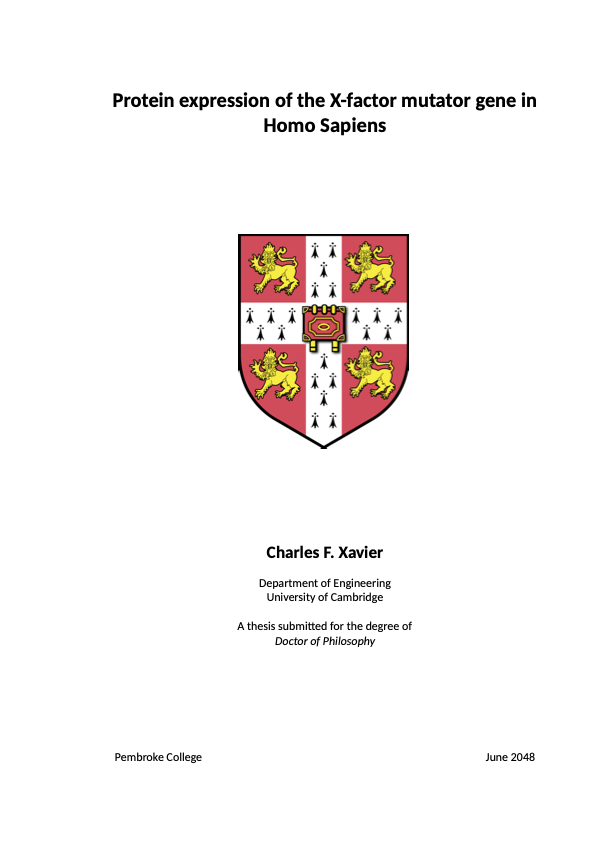
\includegraphics[width=0.7\linewidth]{cambridge_phd-title_page}
    \caption[Example of a title page for the University of Cambridge]
    {
        Example of a title page for the University of Cambridge.
        \label{fig:ch0:cambridge_phd-title_page}
    }
\end{figure}


The OxEngThesis class makes available new LaTeX commands that you can use in your new custom title document. These new commands are based on the variables defined in the preamble of your ``\textit{main LaTeX source file}'':


\begin{itemize}

    \item The \verb|\title{}| variable in the preamble will map to the command \verb|\TitleName|

    \item The \verb|\author{}| variable in the preamble will map to the command \verb|\AuthorName|

    \item The \verb|\supervisor{}| variable in the preamble will map to the command \verb|\SupervisorName|

    \item The \verb|\college{}| variable in the preamble will map to the command \verb|\CollegeName|

    \item The \verb|\degreeprefix{}| variable in the preamble will map to the command \verb|\DegreePrefix|

    \item The \verb|\degree{}| variable in the preamble will map to the command \verb|\DegreeName|

    \item The \verb|\department{}| variable in the preamble will map to the command \verb|\DepartmentName|

    \item The \verb|\university{}| variable in the preamble will map to the command \verb|\UniversityName|

    \item The \verb|\universitylogo{}| variable in the preamble will map to the command \verb|\UniversityLogo|

    \item The \verb|\date{}| variable in the preamble will map to the command \verb|\DegreeDate|

\end{itemize}


Check the files ``\verb|titlepage-oxford.tex|'', ``\verb|titlepage-mit.tex|'' and ``\verb|titlepage-cambridge.tex|'' for examples on how to use the available commands in your new title page.


\section{Package options}


\subsection{Default options}


By default, the class is formatted to produce a doctoral thesis for the University of Oxford. If you don't provide any package options in your ``\textit{main LaTeX source file}'' (as it is written in the \verb|sample_dphil_thesis.tex| file provided in this repository), such as:


\begin{lstlisting}[style=custom-latex]
\documentclass{oxengthesis}
\end{lstlisting}


\noindent the following options will be used:


\begin{lstlisting}[style=custom-latex]
\documentclass[10pt,a4paper,openany,onecolumn,twoside,final,font=Carlito,mathfont="Latin Modern Math",headingcolour={0,0,0},leftmargin=4cm,rightmargin=2cm,topmargin=2cm,bottommargin=2.5cm]{oxengthesis}
\end{lstlisting}


\noindent which will produce a thesis using a 10-point Carlito font on A4 paper size. Page margins will be formatted as required by Oxford. Chapters will start on either recto or verso pages (\verb|openany|). Note that the options ``\verb|[onecolumn,twoside,final]|'' cannot be changed.


The OxEngThesis class template is based on the \textit{memoir}\footnote{\url{https://ctan.org/pkg/memoir}} LaTeX package. As such, you can pass most of the \textit{memoir}'s option and, therefore, customise your document even further.


\subsection{Page size and margins}


By default, the page size and margins are set to comply with the requirements of the University of Oxford. Other institutions have different requirements. For example, the requirements for a thesis at the Massachusetts Institute of Technology (taken from MIT libraries\footnote{\url{https://libraries.mit.edu/distinctive-collections/thesis-specs}}) are:


\begin{lstlisting}[style=custom-text]
... For the main body of the text, including appendices and front matter, font size should be at least 11-point ...

... Top, bottom, and both side margins must be at least an inch wide (1″) to allow for binding and trimming....
\end{lstlisting}


Therefore, you would configure the class with the following options (Note that the left margin is larger to account for the thesis binding):


\begin{lstlisting}[style=custom-latex]
\documentclass[11pt,letterpaper,leftmargin=1.5in,rightmargin=1in,topmargin=1in,bottommargin=1in]{oxengthesis}
\end{lstlisting}


\subsection{Fonts}


By default, the main font is 10-point \textit{Carlito}\footnote{\url{https://ctan.org/tex-archive/fonts/carlito}} and the font for equations and formulas is ``\textit{Latin Modern Math}''\footnote{\url{https://ctan.org/tex-archive/fonts/lm-math}}. You can change to, for example, 11pt \verb|Arial| as the main font and ``\verb|tex-gyre-math-termes|'' as the font for equations with the following package options:


\begin{lstlisting}[style=custom-latex]
\documentclass[11pt,font=Arial,mathfont="TeX Gyre Termes Math"]{oxengthesis}
\end{lstlisting}


\subsection{Mini-table of contents for each chapter}


If you have a recent version of LaTeX installed (TeXLive version 2022 works) in your system and would like to have a short table of contents at the beginning of each chapter, you can simply add the ``\verb|chaptertoc|'' option to your document, as in:


\begin{lstlisting}[style=custom-latex]
\documentclass[chaptertoc]{oxengthesis}
\end{lstlisting}


\Cref{fig:ch0:dphil-chap_minitoc} shows a sample output for one chapter. I use the \textit{minitoc}\footnote{\url{https://ctan.org/pkg/memoir}} package to create the table of contents for each chapter. Previous versions of the minitoc class where incompatible with the \textit{memoir} class. I tested TexLive 2022 and MacTeX 2022, they both work fine.


\begin{figure}[htb]
    \centering
    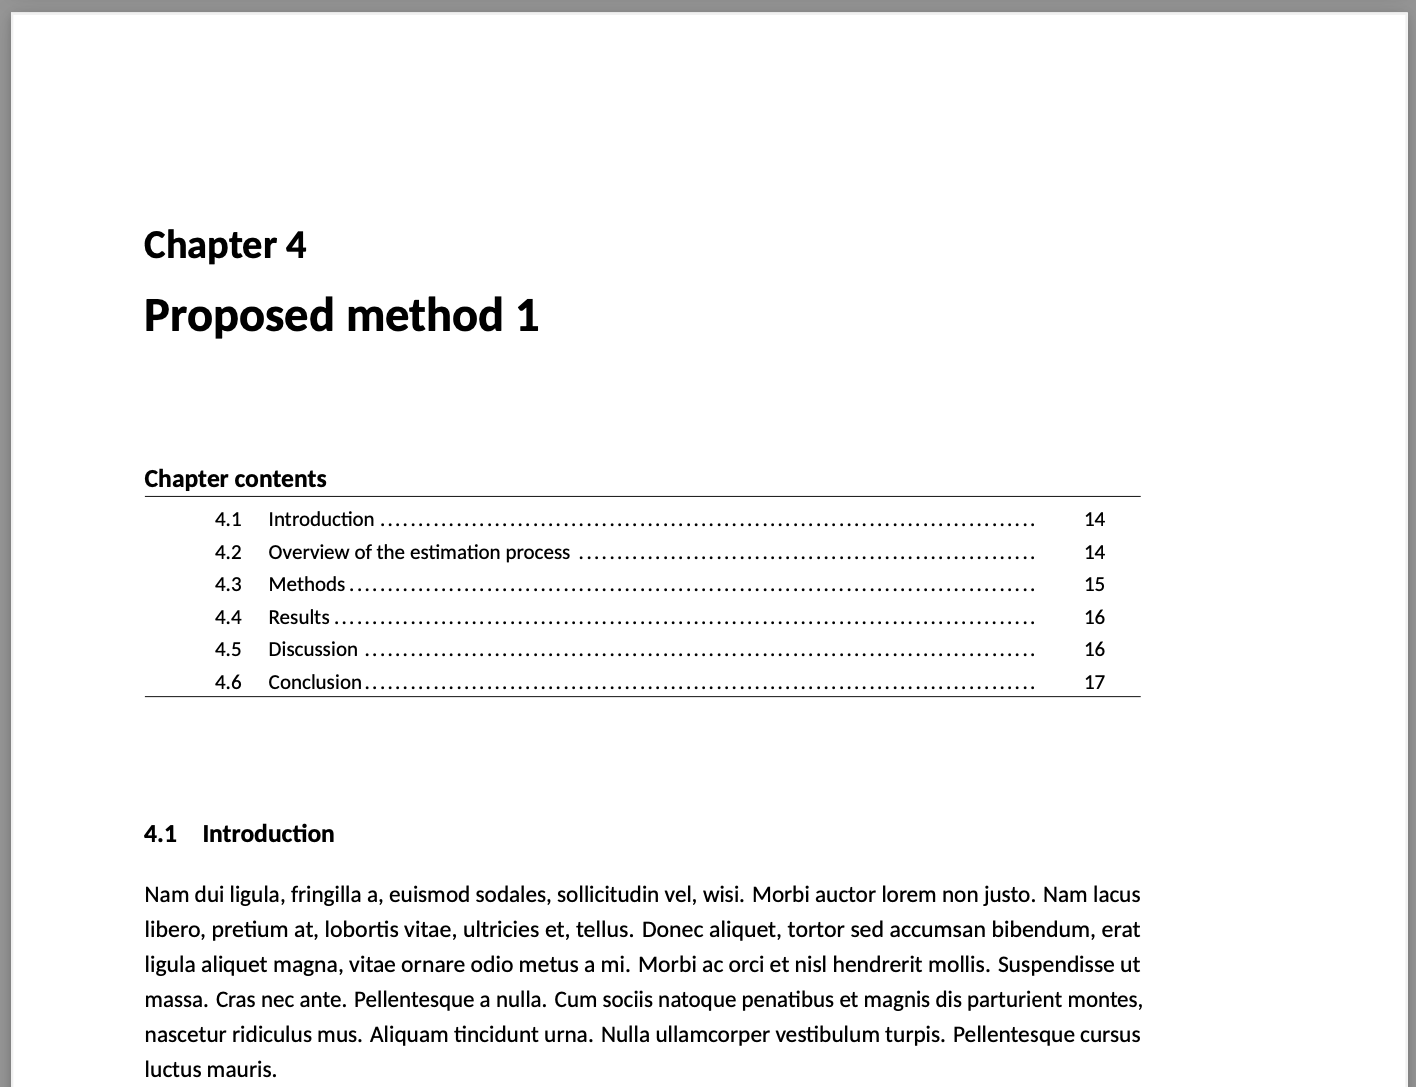
\includegraphics[width=0.7\linewidth]{dphil-chap_minitoc}
    \caption[Example of the table of contents for a chapter]
    {
        Example of the table of contents for a chapter.
        \label{fig:ch0:dphil-chap_minitoc}
    }
\end{figure}


\subsection{Abstract page for the Examination Schools}


When submitting your final thesis to the ``Examination Schools'' (located on High Street) at the University of Oxford to schedule your viva examination, you are typically required to submit two printed copies of your thesis (soft-bound). Additionally, you are required to provide two separate one-page printed copies of your abstract. The stand-alone abstract page should contain your name, college affiliation and is NOT meant to be part of the binding of your thesis. To create this single stand-alone page of your abstract, add the ``\verb|frontabstract|'' option to your document, as shown in the code below. The page will be created before the main title page, as shown in \cref{fig:ch0:dphil-front_abstract_page}.


\begin{lstlisting}[style=custom-latex]
\documentclass[frontabstract]{oxengthesis}
\end{lstlisting}


\begin{figure}[htb]
    \centering
    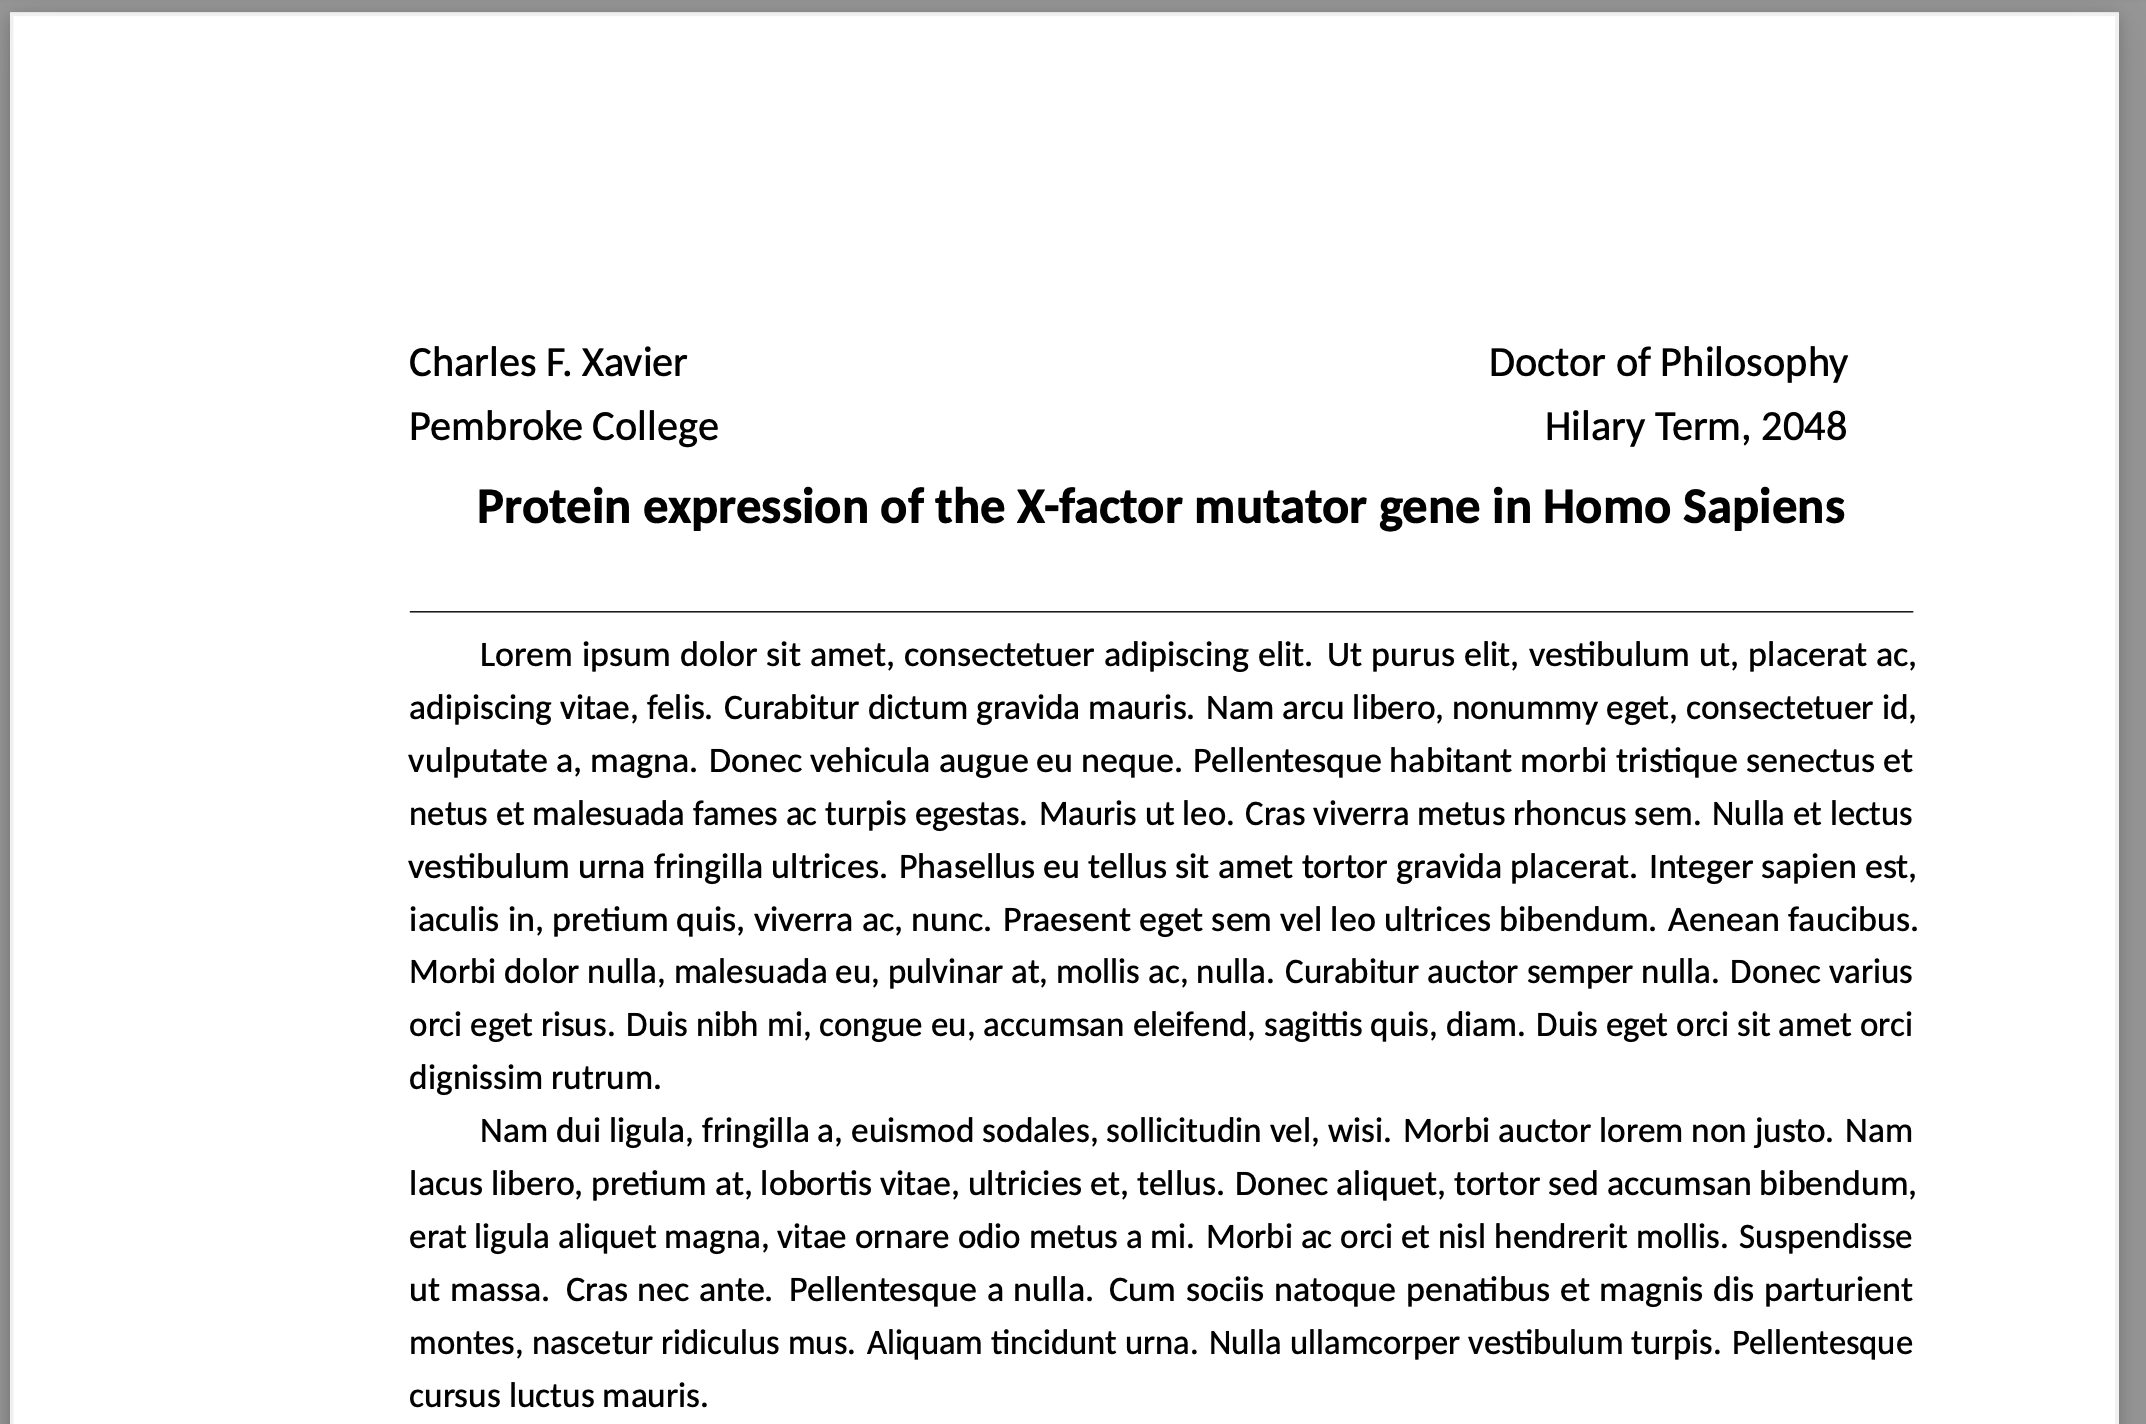
\includegraphics[width=0.7\linewidth]{dphil-front_abstract_page}
    \caption[Example of the abstract page for the Examination Schools]
    {
        Example of the abstract page for the Examination Schools.
        \label{fig:ch0:dphil-front_abstract_page}
    }
\end{figure}


\subsection{Review editing mode}


Your thesis supervisor may request you to print your document with double line spacing so he/she can correct your draft (the \textcolor{red}{red pen!}). You can simply add the ``\verb|review|'' option to your document:


\begin{lstlisting}[style=custom-latex]
\documentclass[review]{oxengthesis}
\end{lstlisting}


\subsection{Different colour for section headings}


The default font colour for section and subsection headings is black. You can change the colour (to blue for example) by adding the ``\verb|headingcolour|'' class option:


\begin{lstlisting}[style=custom-latex]
\documentclass[headingcolour={0.25,0.45,0.76}]{oxengthesis}
\end{lstlisting}


Note that the colour of \verb|\subsubsection| headings will be black regardless of the setting above.


\subsection{Chapter heading styles}


The default style for chapter headings is simple and gives you enough space to write your content. You can take advantage of different chapter styles defined in the \textit{memoir}\footnote{\url{https://ctan.org/pkg/memoir}} package by passing the ``\verb|chapterstyle|'' option. The code shown below will use the ``\verb|southall|'' chapter style to produce the sample \cref{fig:ch0:chapterstyle-southall}.


\begin{lstlisting}[style=custom-latex]
\documentclass[chapterstyle=southall]{oxengthesis}
\end{lstlisting}


\begin{figure}[htb]
    \centering
    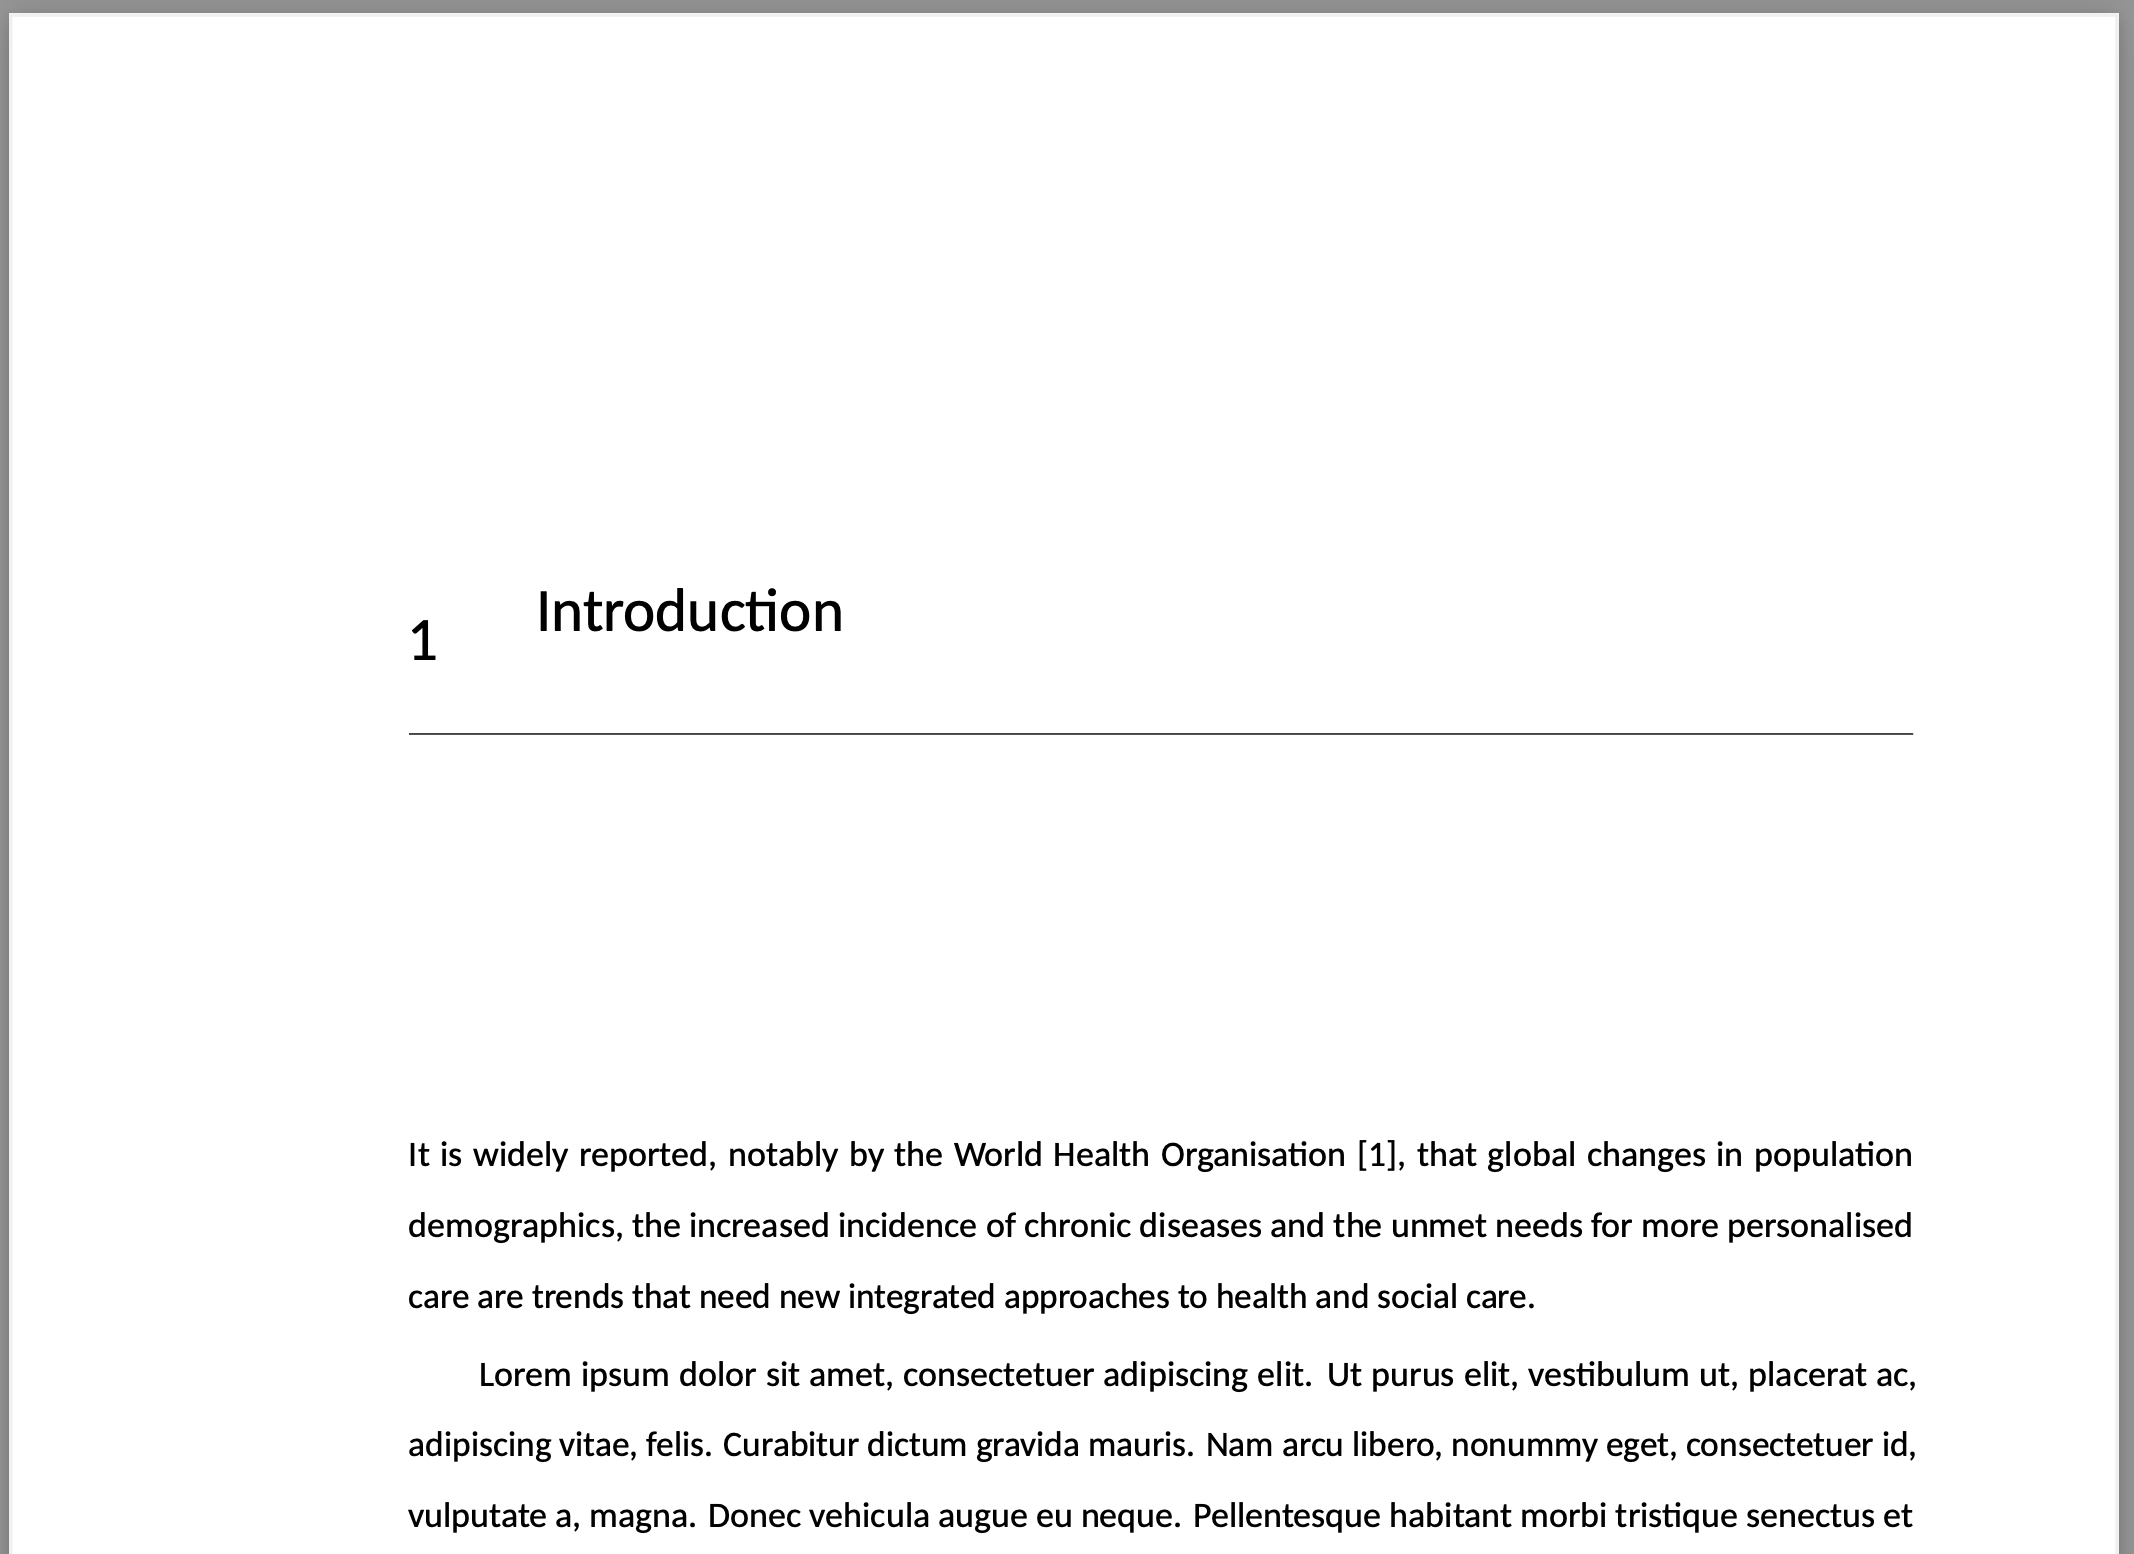
\includegraphics[width=0.7\linewidth]{chapterstyle-southall}
    \caption[The southall chapter heading style]
    {
        The southall chapter heading style.
        \label{fig:ch0:chapterstyle-southall}
    }
\end{figure}


\section{Additional features}


This section describes some of the additional features available in the OxEngThesis class. Refer to the official documentation of the \textit{memoir}\footnote{\url{https://ctan.org/pkg/memoir}} LaTeX package to customise your document even further.


\subsection{Figures}


\begin{figure}[htb]
    \centering
    \includegraphics[width=0.5\linewidth]{dummy_image}
    \caption[Sample figure covering 50\% of the page width]
    {
        Sample figure covering 50\% of the page width.
        \label{fig:ch0:sample_image}
    }
\end{figure}


I use the \textit{graphicx}\footnote{\url{https://ctan.org/pkg/graphicx}} package to include figures. You can put all figures in a ``\url{figures/}'' folder and you can simply include the image file directly without the file extension. For example, \cref{fig:ch0:sample_image} shows the image file ``\url{./figures/dummy_image.png}''. You can also create a figure with sub plots, as shown in \cref{fig:ch0:subfig_example}. Note that you can directly refer to the subplot as ``\cref{fig:ch0:subfig_example:fig1}''.


\begin{figure}
    \centering
    \subbottom[\label{fig:ch0:subfig_example:fig1}]{
        \includegraphics[width=0.3\linewidth]{dummy_image}
    }
    \subbottom[\label{fig:ch0:subfig_example:fig2}]{
        \includegraphics[width=0.3\linewidth]{dummy_image}
    }
    \subbottom[\label{fig:ch0:subfig_example:fig3}]{
        \includegraphics[width=0.3\linewidth]{dummy_image}
    }
    \caption[Sample figure with sub figures]
    {
        Sample figure with sub figures, showing:
        \subcaptionref{fig:ch0:subfig_example:fig1} caption for subfigure 1,
        \subcaptionref{fig:ch0:subfig_example:fig2} caption for subfigure 2 and
        \subcaptionref{fig:ch0:subfig_example:fig3} caption for subfigure 3.
        \label{fig:ch0:subfig_example}
    }
\end{figure}


\subsection{Tables}


\begin{table}[htb]
    \centering
    \caption{General features and specification for ...}
    \singleTableRowHeight
    \begin{tabular}{ll}

        \tableHeaderStart
        \tableHCell{Item} & \tableHCell{Description} \\
        \tableHeaderEnd

        Imaging Sensor        & Sony ICX625 2/3" progressive scan CCD \\
        Image size (pixels)   & 2448 (H) x 2048 (V)                   \\
        Pixel Size            & 3.45 \si{\micro\metre} x 3.45 \si{\micro\metre} \\
        A/D Converter         & AD9977 14-bit, dual-channel           \\
        Max frame rate        & 15 FPS                                \\
        Video Data Output     & 8, 12, 16 and 24-bit digital data     \\
        Gain \& Exposure                  & Automatic/Manual/One-Push \\
        Lens Mount            & C-mount                               \\
        Interface             & Gigabit Ethernet                      \\
        Physical dimensions   & 44 (W) mm x 29 (H) mm x 58 (L) mm     \\
        \hline 

    \end{tabular}
    \label{table:ch0:camera_specs}
\end{table}


You can create tables using the regular syntax in LaTeX. You can also create tables with additional styles. For example, \cref{table:ch0:camera_specs} shows a classical table with shaded headers. You can have more complex tables, as shown in \cref{table:ch0:patient_demographics}


\begin{table}[htb]
  \centering
  \caption{Summary of population demographics in the training and test sets}
  {
    \small
    \begin{tabular}{p{2cm} c c c c c c c c c c}
      \toprule

      Set &
      \multirowcell{2}{Number of\\subjects} &
      \multirowcell{2}{Total time\\(hours)}$^1$ &
      \multicolumn{2}{c}{Gender} &      
      \multicolumn{6}{c}{Ethnicity$^2$}  \\

      \cmidrule{4-11}
        
      &  &  & Male & Female & W & B & A & WB & WA & O  \\
      \midrule
      Training  & 15 & 216.6 & 8  & 7  & 10 & 1   & 1 & 1 & 1 & 1 \\        
      Test      & 15 & 210.0 & 10 & 5  & 10 & $-$ & 1 & 1 & 2 & 1 \\        
      \midrule        
      Total	& 30 & 426.6 & 18 & 12 & 20 & 1   & 2 & 2 & 3 & 2 \\
        
      \bottomrule
        
      \multicolumn{11}{l}
      {
        \footnotesize $^1$ Period during which both reference and estimated data were being recorded simultaneously.        
      } \\        
      \multicolumn{11}{l}
      {        
        \footnotesize $^2$ W = White, B = Black, A = Asian, WB = Mixed White \& Black, WA = Mixed White \& Asian and O = Other.        
      } \\
        
      \end{tabular}      
  } 
  \label{table:ch0:patient_demographics}
\end{table}


\subsection{Cross-referencing labels}


I use the \textit{cleveref}\footnote{\url{https://ctan.org/pkg/cleveref}} package to automatically format the label when cross referencing chapters, sections, figures and other common LaTeX labels. The following paragraphs, show some of the results.

You don't have to include the word ``chapter'': \Cref{chapter:literature_review} discusses .... is presented in \cref{chapter:dataset} with a detailed ...

You don't have to include the word ``figure'' or ``table'': The summary of the demographics for the entire set is described in \cref{table:ch0:patient_demographics} ... \Cref{fig:ch0:subfig_example} shows the video camera used in the study. \Cref{fig:ch0:subfig_example:fig1} shows the the camera model used, \cref{fig:ch0:subfig_example:fig2} shows the ... and \cref{fig:ch0:subfig_example:fig3} shows...


\subsection{Glossary, acronyms and abbreviations}


I use the \textit{glossaries-extra}\footnote{\url{https://ctan.org/pkg/glossaries-extra}} packages to define acronyms and automatically add the ``Glossary'' page in the \textit{frontmatter}. Simply create a file with the name ``glossary.tex'' and add all your definitions to it. Note that the first time you use an acronym, its full definition will be provided. For the rest of the instances, only the abbreviation will be used. The following paragraphs show how to define and use acronyms.

The standard vital signs include temperature, \ab{hr}, \ab{rr}, \ab{bp} and, when appropriate, \ab{spo2}. The routine measurement and interpretation of these vital signs is a core component of the physiological assessment of most patients \cite{prior1977physical,goldberg2005practical} as they can provide critical information about the underlying state of their health. 

We included all study types looking at monitoring of \ab{hr}, \ab{bp}, \ab{rr} or \ab{spo2} using image analysis with comparison to a reference device. We did not restrict based on clinical setting and included all age groups. Only non-contact methods using cameras were included. All unpublished studies found were included wherever possible to minimise publication bias.


\subsection{Citations and references}


This section contains example on how to cite papers, journals and other documents:

It is widely reported, notably by the World Health Organisation \cite{stroetmann2010can}, that global changes in population demographics, the increased incidence of chronic diseases and the unmet needs for more personalised care are trends that need new integrated approaches to health and social care. \cite{brooks1984infrared}


\lipsum[1]\cite{barker1987pulse,peacock1998oxygen,moller1993randomized}


Finding reliable correspondences in two images of a scene taken from arbitrary viewpoints viewed with possibly different cameras and in different illumination conditions is a difficult and critical step towards fully automatic reconstruction of 3D scenes\cite{hartley2003multiple}.


\lipsum[7]\cite{priya2012transition,haralick1973textural,Grass2012Online,NoninPulseOxOnline}


\subsection{Bibliography styles}


The default style for the references is ``\verb|ieeetr|''. For example, the following text: ``\textit{...Finding reliable correspondences in two images of a scene taken from arbitrary viewpoints viewed with possibly different cameras and in different illumination conditions is a difficult and critical step towards fully automatic reconstruction of 3D scenes \cite{hartley2003multiple}...}'' will produce the following output in the bibliography section at the end of the thesis:


\begin{lstlisting}[style=custom-text]
Bibliography
...
[8] R. Hartley and A. Zisserman, Multiple view geometry in computer vision. Cambridge university press, 2003.
...
\end{lstlisting}


You can specify a custom bibliography style as an argument to the ``\verb|\listofreferences|'' command in your \textit{main LaTeX source file}. For example, the following command:


\begin{lstlisting}[style=custom-latex]
\listofreferences[apalike]
\end{lstlisting}


\noindent will use the \textit{apalike}\footnote{\url{https://www.bibtex.com/s/bibliography-style-base-apalike}}
BibTeX style and produce the following output in the content pages:


\begin{lstlisting}[style=custom-text]
...Finding reliable correspondences in two images of a scene taken from arbitrary viewpoints viewed with possibly different cameras and in different illumination conditions is a difficult and critical step towards fully automatic reconstruction of 3D scenes [Hartley and Zisserman, 2003]...
\end{lstlisting}


\noindent and the bibliography section will read:


\begin{lstlisting}[style=custom-text]
Bibliography
...
[Hartley and Zisserman, 2003] Hartley, R. and Zisserman, A. (2003). Multiple view geometry in computer vision. Cambridge university press.
...
\end{lstlisting}

Take a look at the available styles at \textit{The quick BibTeX guide}\footnote{\url{https://www.bibtex.com/styles}} online.


\subsection{Mark text as TODO}


You can wrap text in``todo'' tags, so they appear in red colour in the PDF document. For example:

\todo{This text is in red colour, it reminds me of a task to complete}


\subsection{Formatting source code}


Often, we want to show pseudo code, source code or other verbatim content in our document. For this, I use the \textit{listings}\footnote{\url{https://ctan.org/pkg/listings}} package. The extra custom styles defined in the OxEngThesis class file are:


Example on displaying C/C++ source code:


\begin{lstlisting}[style=custom-c,caption={Function to balance a matrix.}]
extern PE_SIGPROC_API void pesig_balance(
        const size_t    n,
        signal_value_t  A[n][n],
        signal_value_t* S
        );
\end{lstlisting}


Example on displaying BASH/Console scripts:


\begin{lstlisting}[style=custom-bash,caption={A script in bash.}]
$ mkdir -p $HOME/code/pebase/realtime
$ cd $HOME/code/pebase/realtime
$ git clone git@github.com:maurovm/thesis_template.git repository
\end{lstlisting}


Example of displaying text as ``verbatim'' mode:


\begin{lstlisting}[style=custom-verbatim,caption={License information.}]
OxEngThesis is provided under:

    SPDX-License-Identifier:    GPL-2.0-only
    
OxEngThesis is free software: you can redistribute it or modify
it under the terms of the GNU General Public License as published by the
Free Software Foundation, version 2 only, according with:

    LICENSES/GPL-2.0

OxEngThesis is distributed in the hope that it will be useful, but
WITHOUT ANY WARRANTY; without even the implied warranty of MERCHANTABILITY
or FITNESS FOR A PARTICULAR PURPOSE. See the GNU General Public License
for more details.
\end{lstlisting}


\subsection{Coloured boxes}


I use the \textit{tcolorbox}\footnote{\url{https://ctan.org/pkg/tcolorbox}} package to show coloured and framed text boxes with an optional heading line. Some examples include:

\noindent Standard box:


\begin{tcolorbox}
\lipsum[1]
\end{tcolorbox}


\noindent Standard box with title:


\begin{tcolorbox}[title=Box title]
\lipsum[1]
\end{tcolorbox}


\noindent A small box following text:\dotfill\tcbox[nobeforeafter,colframe=blue!50!black,colback=white,colupper=red!50!black]{Hello World}\hfill


Read the documentation of the \verb|tcolorbox| package to see an extensive description of the configuration options and what you can do with the \verb|tcolorbox| class, it is quite customisable. The OxEngThesis class defines some environment commands for some predefined boxes. For example, the following is a warning box:


\begin{OxWarningBox}{Warning box title}
Warning box content: \lipsum[1]
\end{OxWarningBox}


The following example shows an information box:


\begin{OxInfoBox}{Informational box title}
Warning box content: \lipsum[1]
\end{OxInfoBox}


\section{Troubleshooting common errors}


\subsection{Text beyond page limits}


When compiling a LaTeX document, you could get a warning similar to:


\begin{lstlisting}[style=custom-text]
Overfull \hbox (22.49216pt too wide) in paragraph at lines 4--5
\end{lstlisting}


This often occurs when a line of your document could not fit within the designated horizontal space for text in the current page layout. The LaTeX compiler tries its best to fit text within the page limits, but sometimes it just cannot do it appropriately. This typically results in some text hanging out past the page margin due to long words, acronyms or long equations. Sometimes, it is difficult to know where these errors occur in your document. You can add the ``\verb|debuglayout|'' option to your document:


\begin{lstlisting}[style=custom-latex]
\documentclass[debuglayout]{oxengthesis}
\end{lstlisting}


\begin{figure}[htb]
    \centering
    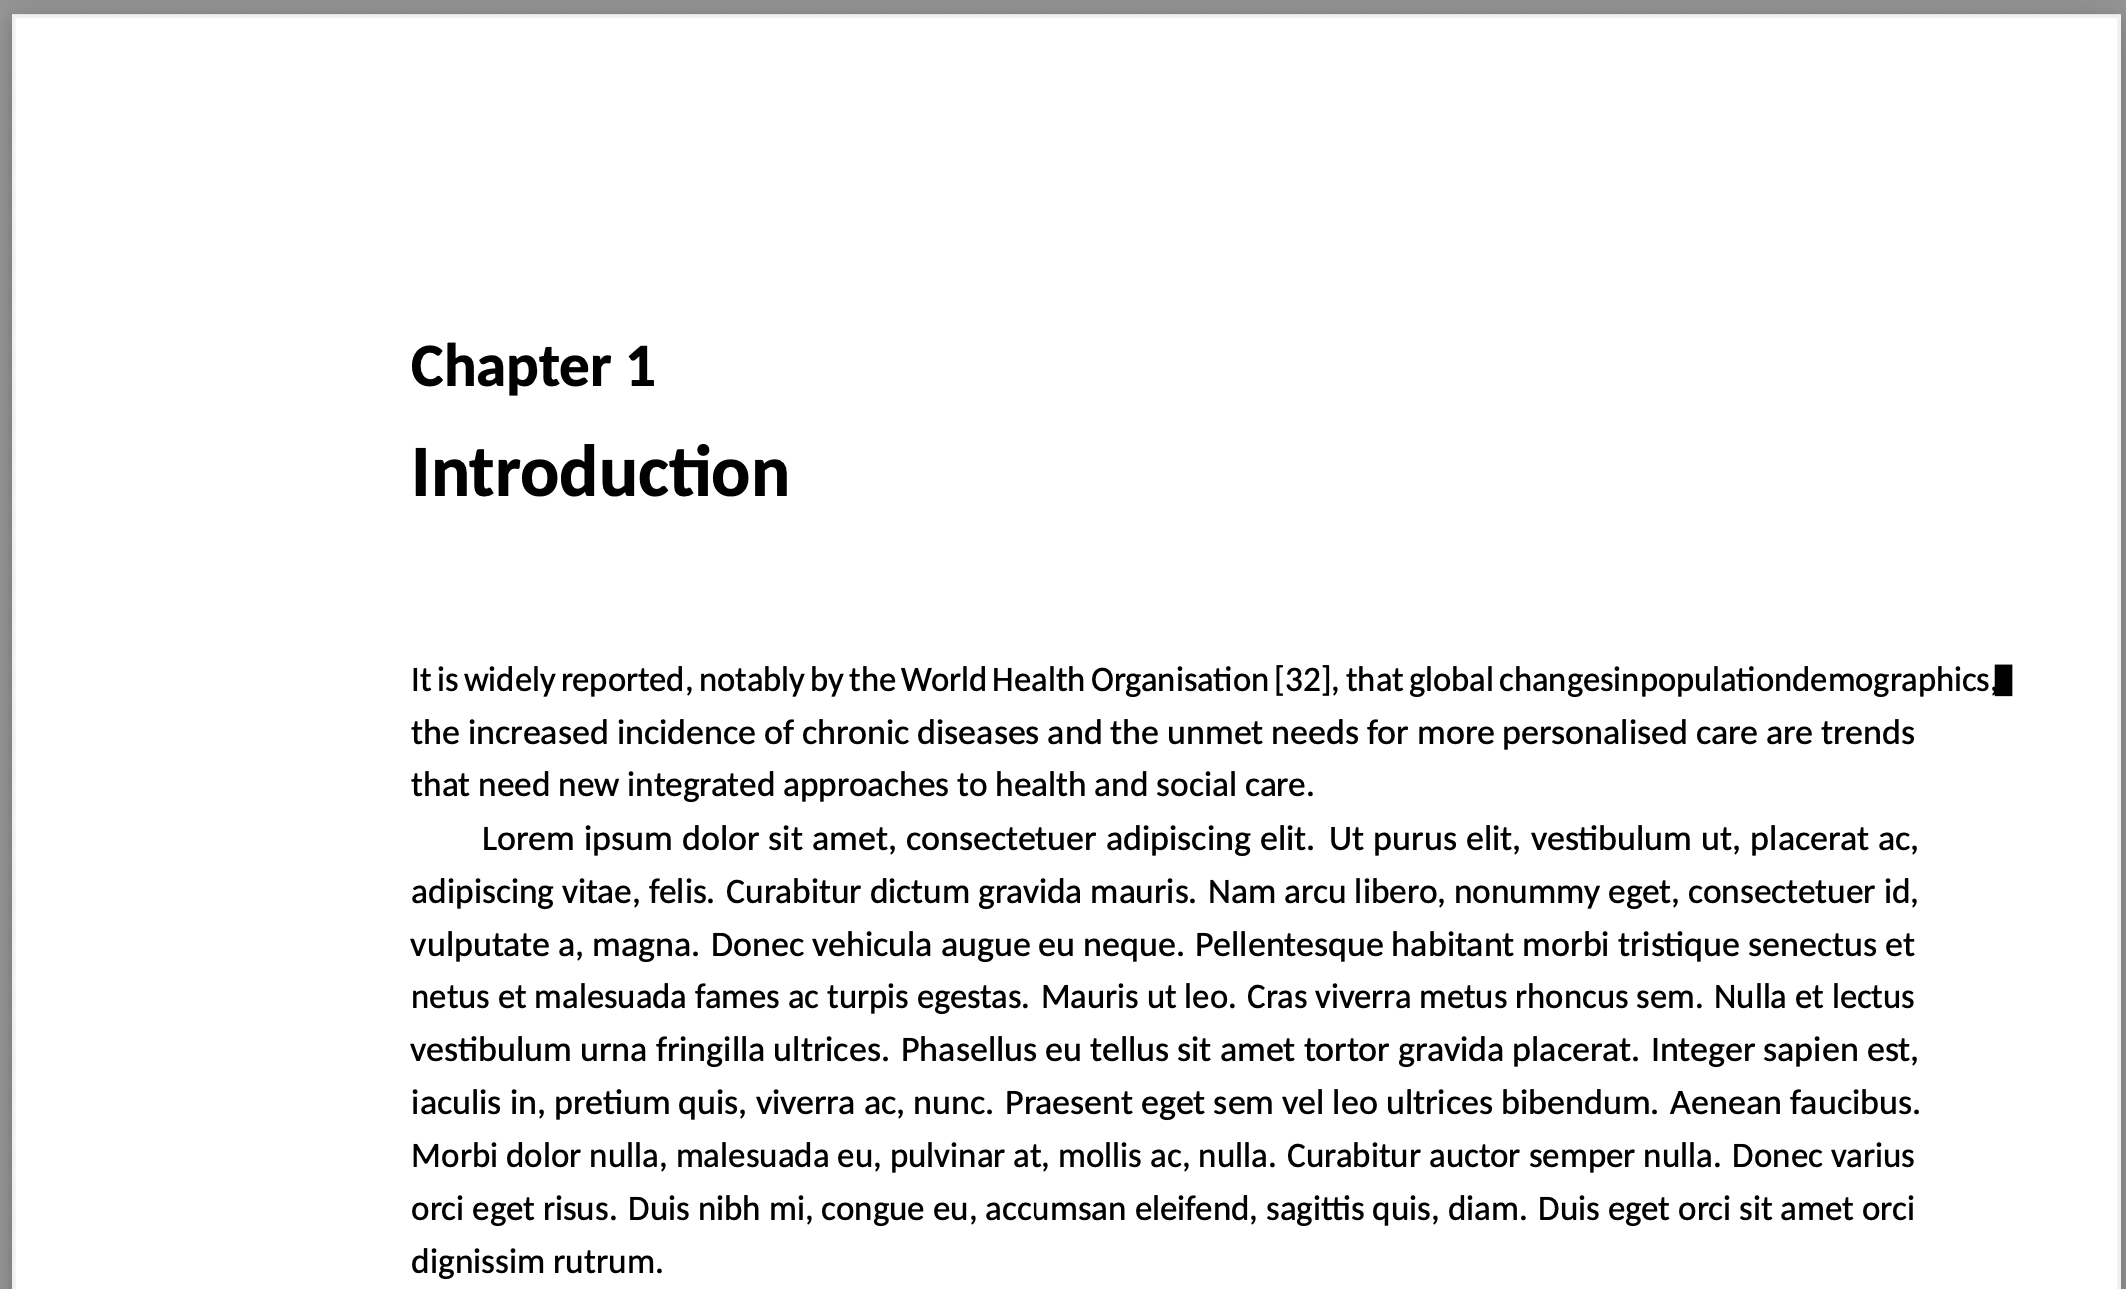
\includegraphics[width=0.7\linewidth]{overfull_hbox_warning}
    \caption[Example of a line of text that does not fit within the horizontal space for text]
    {
        Example of a line of text that does not fit within the horizontal space for text. A black box is shown next to the affected line.
        \label{fig:ch0:overfull_hbox_warning}
    }
\end{figure}


A black box will be shown next to the affected lines, as shown in \cref{fig:ch0:overfull_hbox_warning}. The \url{oxengthesis.cls} class file already takes advantage of other packages (such as \textit{microtype}\footnote{https://ctan.org/pkg/microtype}) to deal with common issues such as character protrusion, font expansion and inter-word spacing. I recommend you slightly rephrase your guilty sentences instead of changing the class template. This is usually the first approach many of my students take.


\end{lstlisting}


Note that the line above includes the chapter you are currently reading. It is only meant to showcase the features provided by the OxEngThesis class. It is numbered as ``Chapter 0'' so not to change the flow of the rest of the document.

The \textit{frontmatter} of the thesis will be automatically created depending on the type of document you are writing, either a doctoral thesis or a project report. If you want more control, you can review how the \verb|\makefrontmatterpages| command is defined in the \verb|oxengthesis.cls| class file. If you want all the sections in the \textit{frontmatter} to appear, you will need to create the following files:


\begin{itemize}
    \item \verb|abstract.tex|: If you want the ``Abstract'' page
    \item \verb|dedication.tex|: If you want the ``Dedication'' page
    \item \verb|declaration.tex|: If you want the ``Declaration'' page
    \item \verb|acknowledgements.tex|: If you want the ``Acknowledgements'' page
    \item \verb|publications.tex|: If you want the ``List of publications'' page
    \item \verb|glossary.tex|: If you want the ``List of abbreviations'' page
\end{itemize}


If any of the files above is missing, that particular page won't be created in the \textit{frontmatter}. This is useful if you are just preparing a draft version of your thesis for your supervisor to correct. 

Similarly for the \textit{backmatter} part of your thesis, add all the BibTeX citations to a file named \verb|references.bib| if you want the ``Bibliography'' section to be created at the end of your document. 


\subsection{Writing a ``Transfer of Status'' or ``Confirmation of Status'' report}


There are two Key milestones\footnote{\url{https://www.ox.ac.uk/students/academic/guidance/graduate/research/status/DPhil}} for which DPhil students are expected to submit substantial piece of written research work, or reports. They are the ``Transfer of Status''\footnote{\url{https://www.mpls.ox.ac.uk/graduate-school/information-and-resources-for-supervisors/transfer-of-status}} at the end of your first year, and the ``Confirmation of Status''\footnote{\url{https://www.mpls.ox.ac.uk/graduate-school/information-and-resources-for-supervisors/confirmation-of-status}} at the end of your second year. 

For these milestones, you will often be required to submit a report with all the details of your research contributions. This document is often around 50-60 pages in length and does not need all the sections that a doctoral thesis has (i.e. declaration, dedication or list of publications). 

You can write a \textit{Transfer of Status} report by simply providing the ``\verb|report|'' option when you load the \verb|OxEngThesis| class, and defining the ``\verb|degree|'' variable as shown in the following code snippet:


\begin{lstlisting}[style=custom-latex]
\documentclass[report]{oxengthesis}

\title       {The title of your report}
\author      {Your name}
\degree      {{\huge Transfer of Status Report}}
\college     {The name of your college}
\supervisor  {The name(s) of your supervisor(s)}
\date        {The academic term of submission}
\end{lstlisting}


You can write a \textit{Confirmation of Status} report by simply providing the ``\verb|report|'' option when you load the \verb|OxEngThesis| class, and defining the ``\verb|degree|'' variable as shown in the following code snippet:


\begin{lstlisting}[style=custom-latex]
\documentclass[report]{oxengthesis}

\title       {The title of your report}
\author      {Your name}
\degree      {{\huge Confirmation of Status Report}}
\college     {The name of your college}
\supervisor  {The name(s) of your supervisor(s)}
\date        {The academic term of submission}
\end{lstlisting}


Note that the "*report*" package option is just a shortcut to not include the dedication, declaration and publications pages and format the title page accordingly.


\subsection{Writing a 4$^{th}$-Year Project (4YP) report}


If you are an undergraduate student at the University of Oxford reading Engineering Science\footnote{\url{https://eng.ox.ac.uk/study/undergraduate/your-degree}}, you will carry out a self-led project during your fourth year. It usually involves original research or significant design and construction work, undertaken in close consultation with an academic supervisor. At the end of your project (usually by the beginning of Trinity term), you will need to submit a report with all the details of your research contributions. This document is often about 50 pages in length and does not need all the sections that a doctoral thesis has (i.e. declaration, dedication or list of publications). 

You can write a 4YP report by simply providing the ``\verb|report|'' option when you load the \verb|OxEngThesis| class, and defining the ``\verb|degree|'' variable as shown in  the following code snippet:


\begin{lstlisting}[style=custom-latex]
\documentclass[report]{oxengthesis}

\title       {The title of your report}
\author      {Your name}
\degree      {{\huge 4$^{th}$ Year Project Report}}
\college     {The name of your college}
\supervisor  {The name(s) of your supervisor(s)}
\date        {The academic term of submission}
\end{lstlisting}


\subsection{Creating the PDF output}


The source files in this repository require the LuaLaTeX engine. You editor should allow you to configure LuaLaTeX as the typesetting engine for your document and automatically take care of the compilation process to generate the final PDF document from your ``\textit{main LaTeX source file}''.

If you want to compile your ``\textit{main LaTeX source file}'' from the command line, you can use the ``\verb|compile_document.sh|'' script provided in this repository. This script only works in a Linux or macOS system. For example, to compile the sample thesis provided, you will execute the following command in the terminal:


\begin{lstlisting}[style=custom-bash]
$ ./compile_document.sh  sample_dphil_thesis.tex
\end{lstlisting}


If you want to delete all the temp or auxiliary files LaTeX created during the compilation process, you can run:


\begin{lstlisting}[style=custom-bash]
$ ./remove_latex_aux_files.sh
\end{lstlisting}


If you are compiling the document manually, you would need to run the \textit{latexmk}\footnote{\url{https://ctan.org/pkg/latexmk}} build command (already part of your LaTeX distribution) in the following order:


\begin{lstlisting}[style=custom-bash]
$ latexmk -pdflatex=lualatex -pdf  sample_dphil_thesis.tex
$ makeglossaries sample_dphil_thesis.tex
$ latexmk -pdflatex=lualatex -pdf  sample_dphil_thesis.tex
\end{lstlisting}


\subsection{Customising the title page}


Although I originally wrote this LaTeX template for a student at the University of Oxford, it should be easy for you to customise it to suit the requirements of your academic institution. The default title page ``\verb|titlepage-oxford.tex|'' is simple and customisable. The class template defines some variables you can use. At minimum, you need to provide the following definitions in the preamble of your ``\textit{main LaTeX source file}'':


\begin{itemize}

    \item \verb|\title{}|: The main title of the thesis/report
    \item \verb|\author{}|: The author of the thesis/report

\end{itemize}

You can define the following optional variables:

\begin{itemize}

    \item \verb|\supervisor{}|: The name of your thesis supervisor. The default value is: ``SUPERVISOR NAME''

    \item \verb|\college{}|: Your college affiliation, if you are an Oxford student. The default value is: ``'' (an \textit{empty string})

    \item \verb|\degreeprefix{}|: Text printed before the degree name. The default value is: ``A thesis submitted for the degree of''

    \item \verb|\degree{}|: The name of the degree. The default value is: ``Doctor of Philosophy''

    \item \verb|\department{}|: Your university department. The default value is: ``Department of Engineering Science''

    \item \verb|\university{}|: The name of your university. The default value is: ``University of Oxford''

    \item \verb|\universitylogo{}|: File name of the university's logo, without the file extension. The default value is: ``oxford-logo'' (which will load the image file \verb|oxford-logo.png| in the \verb|./figures/| folder in this repository

    \item \verb|\date{}|: The date of publication of the thesis, such as ``Hilary Term, 2048''. If you leave it blank, it will print the current date (useful when sending a draft to your supervisor)

\end{itemize}



\begin{figure}[htb]
    \centering
    \subbottom[\label{fig:ch0:title_page:dphil}]{
        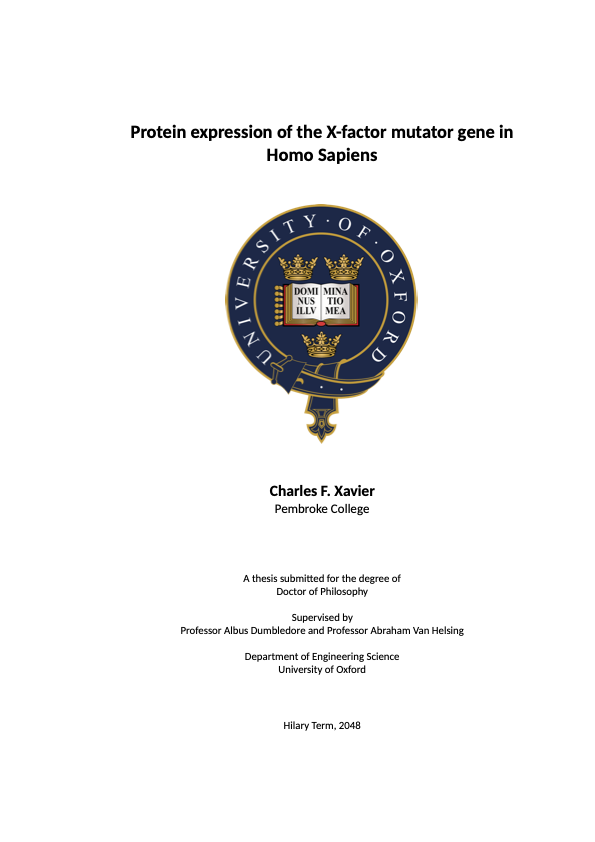
\includegraphics[width=0.45\linewidth]{dphil-title_page}
    }
    \subbottom[\label{fig:ch0:title_page:4yp}]{
        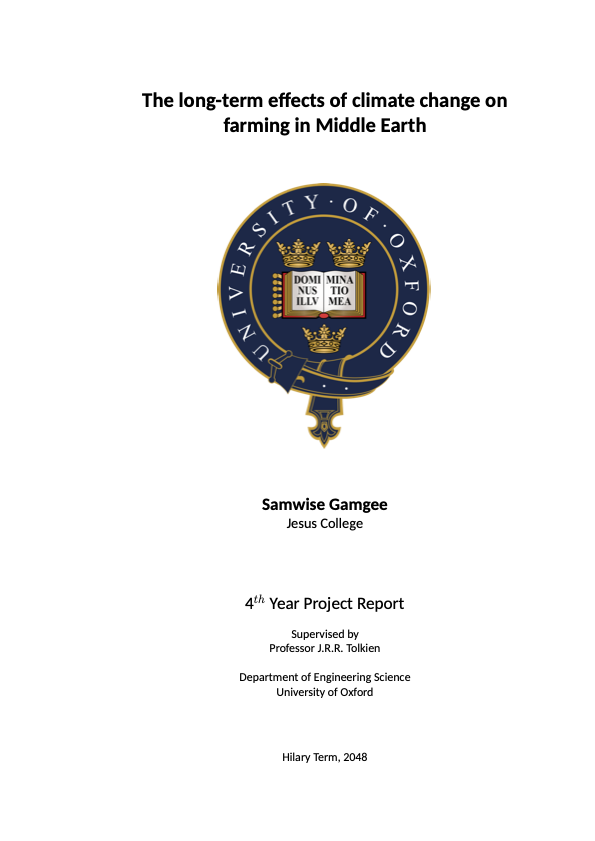
\includegraphics[width=0.45\linewidth]{4yp-title_page}
    }
    \caption[Examples of title pages for a DPhil thesis and a 4$^{th}$ Year Project report]
    {
        Examples of title pages for a \subcaptionref{fig:ch0:title_page:dphil} DPhil thesis and a
        \subcaptionref{fig:ch0:title_page:4yp} 4$^{th}$ Year Project report.
        \label{fig:ch0:title_page}
    }
\end{figure}


\Cref{fig:ch0:title_page} shows examples of the title pages for a DPhil thesis and for a 4YP report using the default title page (file``\verb|titlepage-oxford.tex|''). Both title pages were created with similar code with the ``\verb|report|'' package option as the only difference. The title page for the DPhil thesis (see \cref{fig:ch0:title_page:dphil}) was created with the following code:


\begin{lstlisting}[style=custom-latex]
\documentclass{oxengthesis}

\title{The long-term effects of climate change on farming in Middle Earth}
\author    {Samwise Gamgee}
\college   {Jesus College}
\supervisor{Professor J.R.R. Tolkien}
\date      {Hilary Term, 2048}
\end{lstlisting}


\noindent The title page for the 4YP report (see \cref{fig:ch0:title_page:4yp}) was created with the following code:


\begin{lstlisting}[style=custom-latex]
\documentclass[report]{oxengthesis}

\title{The long-term effects of climate change on farming in Middle Earth}
\author    {Samwise Gamgee}
\college   {Jesus College}
\supervisor{Professor J.R.R. Tolkien}
\date      {Hilary Term, 2048}
\end{lstlisting}


\subsection{Creating your own title page}


If you don't provide a custom title page, the OxEngThesis class will load the default title file ``\verb|titlepage-oxford.tex|'' shown above. If the layout of the default title page does not fulfil your or your university's requirements, you can create your own title page. To do so, you will need to follow the 3 steps described below. As an example, we will create a custom title page for a PhD thesis for a student at the Massachusetts Institute of Technology:

\begin{enumerate}

    \item Create a new LaTeX source file and add your own definitions, such as the example file ``\verb|titlepage-mit.tex|''

    \item Define the \verb|\titlepage{}| variable in the preamble of your ``\textit{main LaTeX source file}''. For example, after the \verb|\author{}| variable as in:


\begin{lstlisting}[style=custom-latex]
\title{Protein expression of the X-factor mutator gene in Homo Sapiens}
\author{Charles F. Xavier}
\titlepage{titlepage-mit.tex}
\end{lstlisting}


    \item Recompile your ``\textit{main LaTeX source file}''. An example of the output is shown in \cref{fig:ch0:mit_phd-title_page}


\end{enumerate}



\begin{figure}[htb]
    \centering
    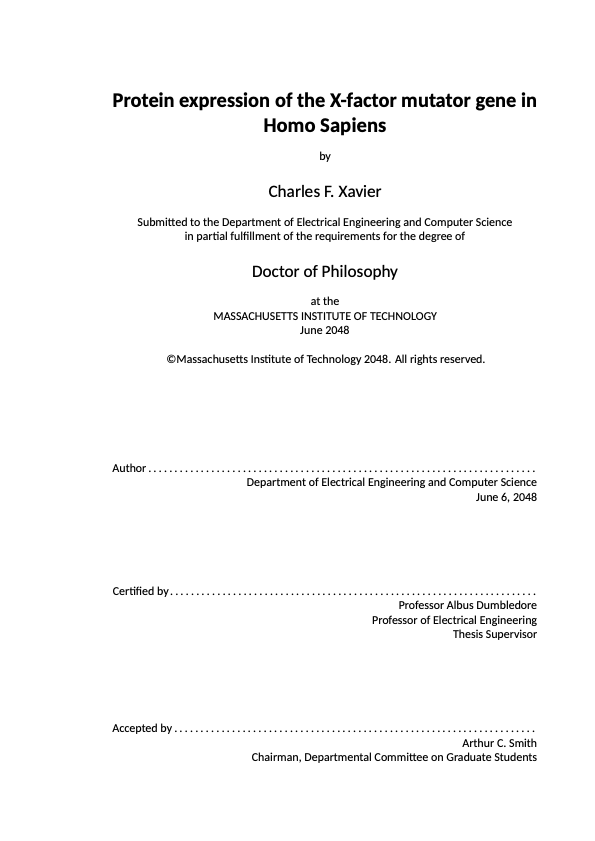
\includegraphics[width=0.7\linewidth]{mit_phd-title_page}
    \caption[Example of a title page for the Massachusetts Institute of Technology]
    {
        Example of a title page for the Massachusetts Institute of Technology.
        \label{fig:ch0:mit_phd-title_page}
    }
\end{figure}


The text below uses the \verb|titlepage-cambridge.tex| file to create a title page for a student at the University of Cambridge. The output is shown in \cref{fig:ch0:cambridge_phd-title_page}.


\begin{lstlisting}[style=custom-latex]
\title{Protein expression of the X-factor mutator gene in Homo Sapiens}
\author     {Charles F. Xavier}
\college    {Pembroke College}
\degreeprefix {A thesis submitted for the degree of}
\degree     {Doctor of Philosophy}
\supervisor {Professor Albus Dumbledore}
\department {Department of Engineering}
\university {University of Cambridge}
\universitylogo{cambridge-logo}
\date       {June 2048}
\titlepage  {titlepage-cambridge.tex}
\end{lstlisting}


\begin{figure}[htb]
    \centering
    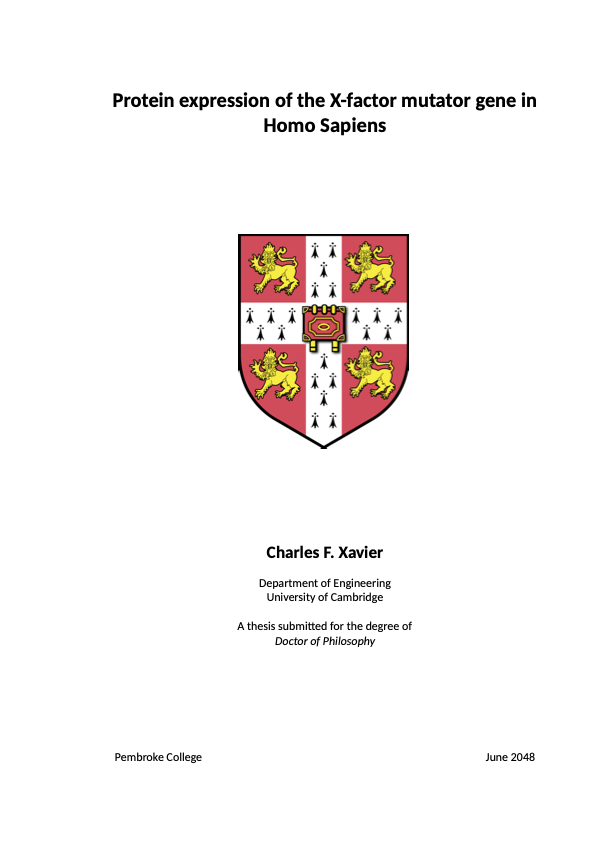
\includegraphics[width=0.7\linewidth]{cambridge_phd-title_page}
    \caption[Example of a title page for the University of Cambridge]
    {
        Example of a title page for the University of Cambridge.
        \label{fig:ch0:cambridge_phd-title_page}
    }
\end{figure}


The OxEngThesis class makes available new LaTeX commands that you can use in your new custom title document. These new commands are based on the variables defined in the preamble of your ``\textit{main LaTeX source file}'':


\begin{itemize}

    \item The \verb|\title{}| variable in the preamble will map to the command \verb|\TitleName|

    \item The \verb|\author{}| variable in the preamble will map to the command \verb|\AuthorName|

    \item The \verb|\supervisor{}| variable in the preamble will map to the command \verb|\SupervisorName|

    \item The \verb|\college{}| variable in the preamble will map to the command \verb|\CollegeName|

    \item The \verb|\degreeprefix{}| variable in the preamble will map to the command \verb|\DegreePrefix|

    \item The \verb|\degree{}| variable in the preamble will map to the command \verb|\DegreeName|

    \item The \verb|\department{}| variable in the preamble will map to the command \verb|\DepartmentName|

    \item The \verb|\university{}| variable in the preamble will map to the command \verb|\UniversityName|

    \item The \verb|\universitylogo{}| variable in the preamble will map to the command \verb|\UniversityLogo|

    \item The \verb|\date{}| variable in the preamble will map to the command \verb|\DegreeDate|

\end{itemize}


Check the files ``\verb|titlepage-oxford.tex|'', ``\verb|titlepage-mit.tex|'' and ``\verb|titlepage-cambridge.tex|'' for examples on how to use the available commands in your new title page.


\section{Package options}


\subsection{Default options}


By default, the class is formatted to produce a doctoral thesis for the University of Oxford. If you don't provide any package options in your ``\textit{main LaTeX source file}'' (as it is written in the \verb|sample_dphil_thesis.tex| file provided in this repository), such as:


\begin{lstlisting}[style=custom-latex]
\documentclass{oxengthesis}
\end{lstlisting}


\noindent the following options will be used:


\begin{lstlisting}[style=custom-latex]
\documentclass[10pt,a4paper,openany,onecolumn,twoside,final,font=Carlito,mathfont="Latin Modern Math",headingcolour={0,0,0},leftmargin=4cm,rightmargin=2cm,topmargin=2cm,bottommargin=2.5cm]{oxengthesis}
\end{lstlisting}


\noindent which will produce a thesis using a 10-point Carlito font on A4 paper size. Page margins will be formatted as required by Oxford. Chapters will start on either recto or verso pages (\verb|openany|). Note that the options ``\verb|[onecolumn,twoside,final]|'' cannot be changed.


The OxEngThesis class template is based on the \textit{memoir}\footnote{\url{https://ctan.org/pkg/memoir}} LaTeX package. As such, you can pass most of the \textit{memoir}'s option and, therefore, customise your document even further.


\subsection{Page size and margins}


By default, the page size and margins are set to comply with the requirements of the University of Oxford. Other institutions have different requirements. For example, the requirements for a thesis at the Massachusetts Institute of Technology (taken from MIT libraries\footnote{\url{https://libraries.mit.edu/distinctive-collections/thesis-specs}}) are:


\begin{lstlisting}[style=custom-text]
... For the main body of the text, including appendices and front matter, font size should be at least 11-point ...

... Top, bottom, and both side margins must be at least an inch wide (1″) to allow for binding and trimming....
\end{lstlisting}


Therefore, you would configure the class with the following options (Note that the left margin is larger to account for the thesis binding):


\begin{lstlisting}[style=custom-latex]
\documentclass[11pt,letterpaper,leftmargin=1.5in,rightmargin=1in,topmargin=1in,bottommargin=1in]{oxengthesis}
\end{lstlisting}


\subsection{Fonts}


By default, the main font is 10-point \textit{Carlito}\footnote{\url{https://ctan.org/tex-archive/fonts/carlito}} and the font for equations and formulas is ``\textit{Latin Modern Math}''\footnote{\url{https://ctan.org/tex-archive/fonts/lm-math}}. You can change to, for example, 11pt \verb|Arial| as the main font and ``\verb|tex-gyre-math-termes|'' as the font for equations with the following package options:


\begin{lstlisting}[style=custom-latex]
\documentclass[11pt,font=Arial,mathfont="TeX Gyre Termes Math"]{oxengthesis}
\end{lstlisting}


\subsection{Mini-table of contents for each chapter}


If you have a recent version of LaTeX installed (TeXLive version 2022 works) in your system and would like to have a short table of contents at the beginning of each chapter, you can simply add the ``\verb|chaptertoc|'' option to your document, as in:


\begin{lstlisting}[style=custom-latex]
\documentclass[chaptertoc]{oxengthesis}
\end{lstlisting}


\Cref{fig:ch0:dphil-chap_minitoc} shows a sample output for one chapter. I use the \textit{minitoc}\footnote{\url{https://ctan.org/pkg/memoir}} package to create the table of contents for each chapter. Previous versions of the minitoc class where incompatible with the \textit{memoir} class. I tested TexLive 2022 and MacTeX 2022, they both work fine.


\begin{figure}[htb]
    \centering
    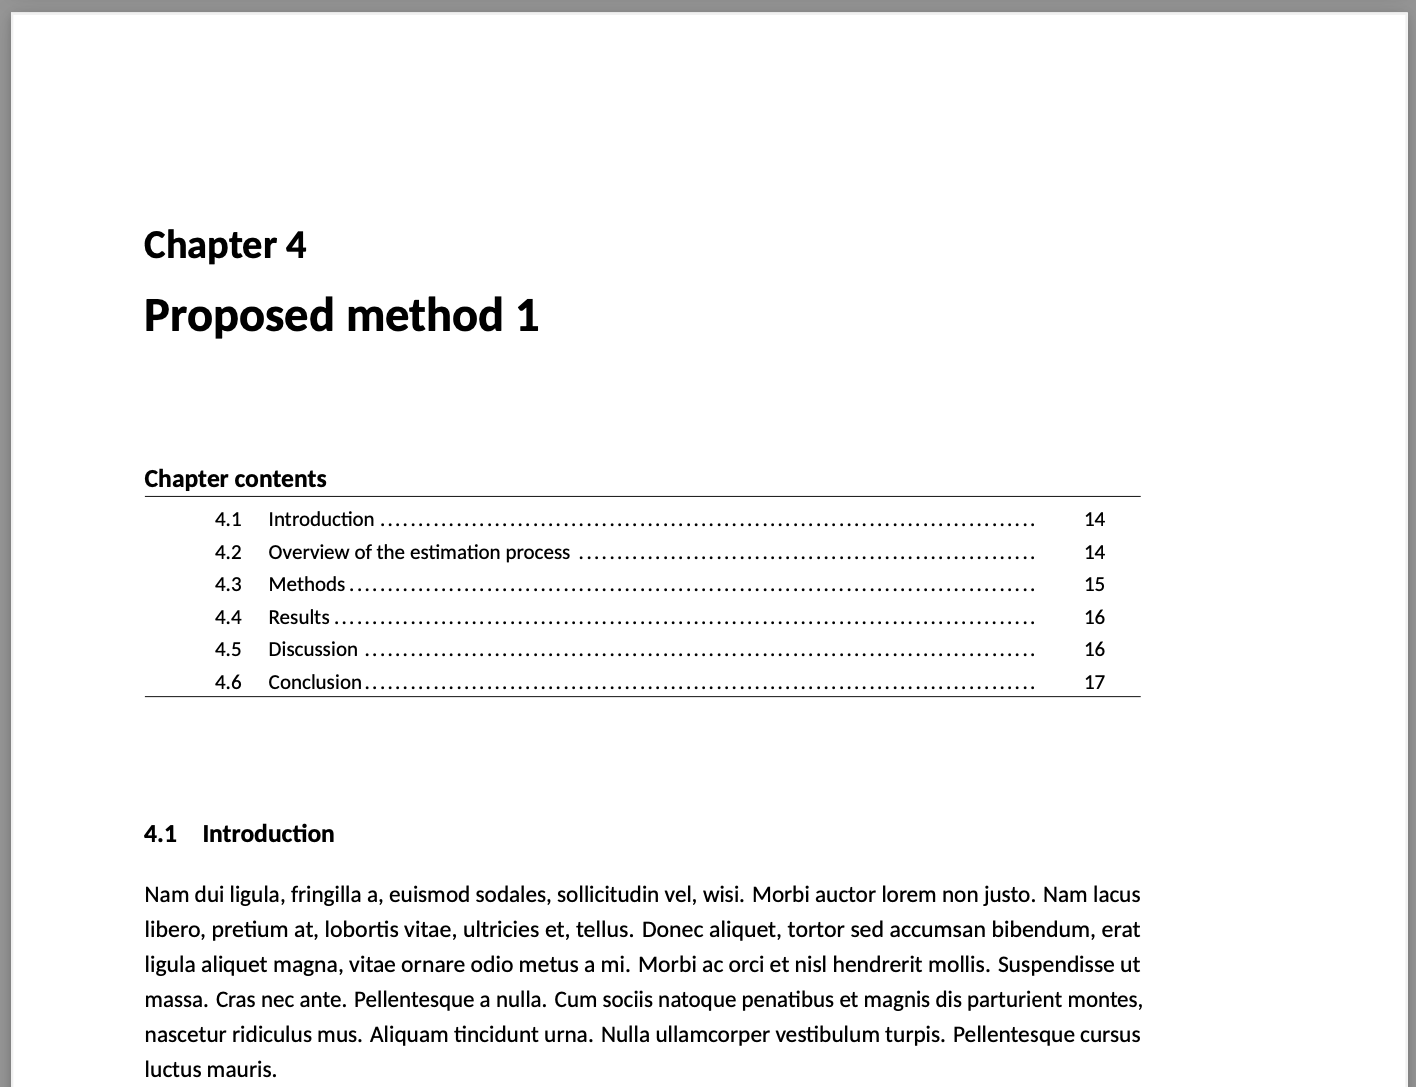
\includegraphics[width=0.7\linewidth]{dphil-chap_minitoc}
    \caption[Example of the table of contents for a chapter]
    {
        Example of the table of contents for a chapter.
        \label{fig:ch0:dphil-chap_minitoc}
    }
\end{figure}


\subsection{Abstract page for the Examination Schools}


When submitting your final thesis to the ``Examination Schools'' (located on High Street) at the University of Oxford to schedule your viva examination, you are typically required to submit two printed copies of your thesis (soft-bound). Additionally, you are required to provide two separate one-page printed copies of your abstract. The stand-alone abstract page should contain your name, college affiliation and is NOT meant to be part of the binding of your thesis. To create this single stand-alone page of your abstract, add the ``\verb|frontabstract|'' option to your document, as shown in the code below. The page will be created before the main title page, as shown in \cref{fig:ch0:dphil-front_abstract_page}.


\begin{lstlisting}[style=custom-latex]
\documentclass[frontabstract]{oxengthesis}
\end{lstlisting}


\begin{figure}[htb]
    \centering
    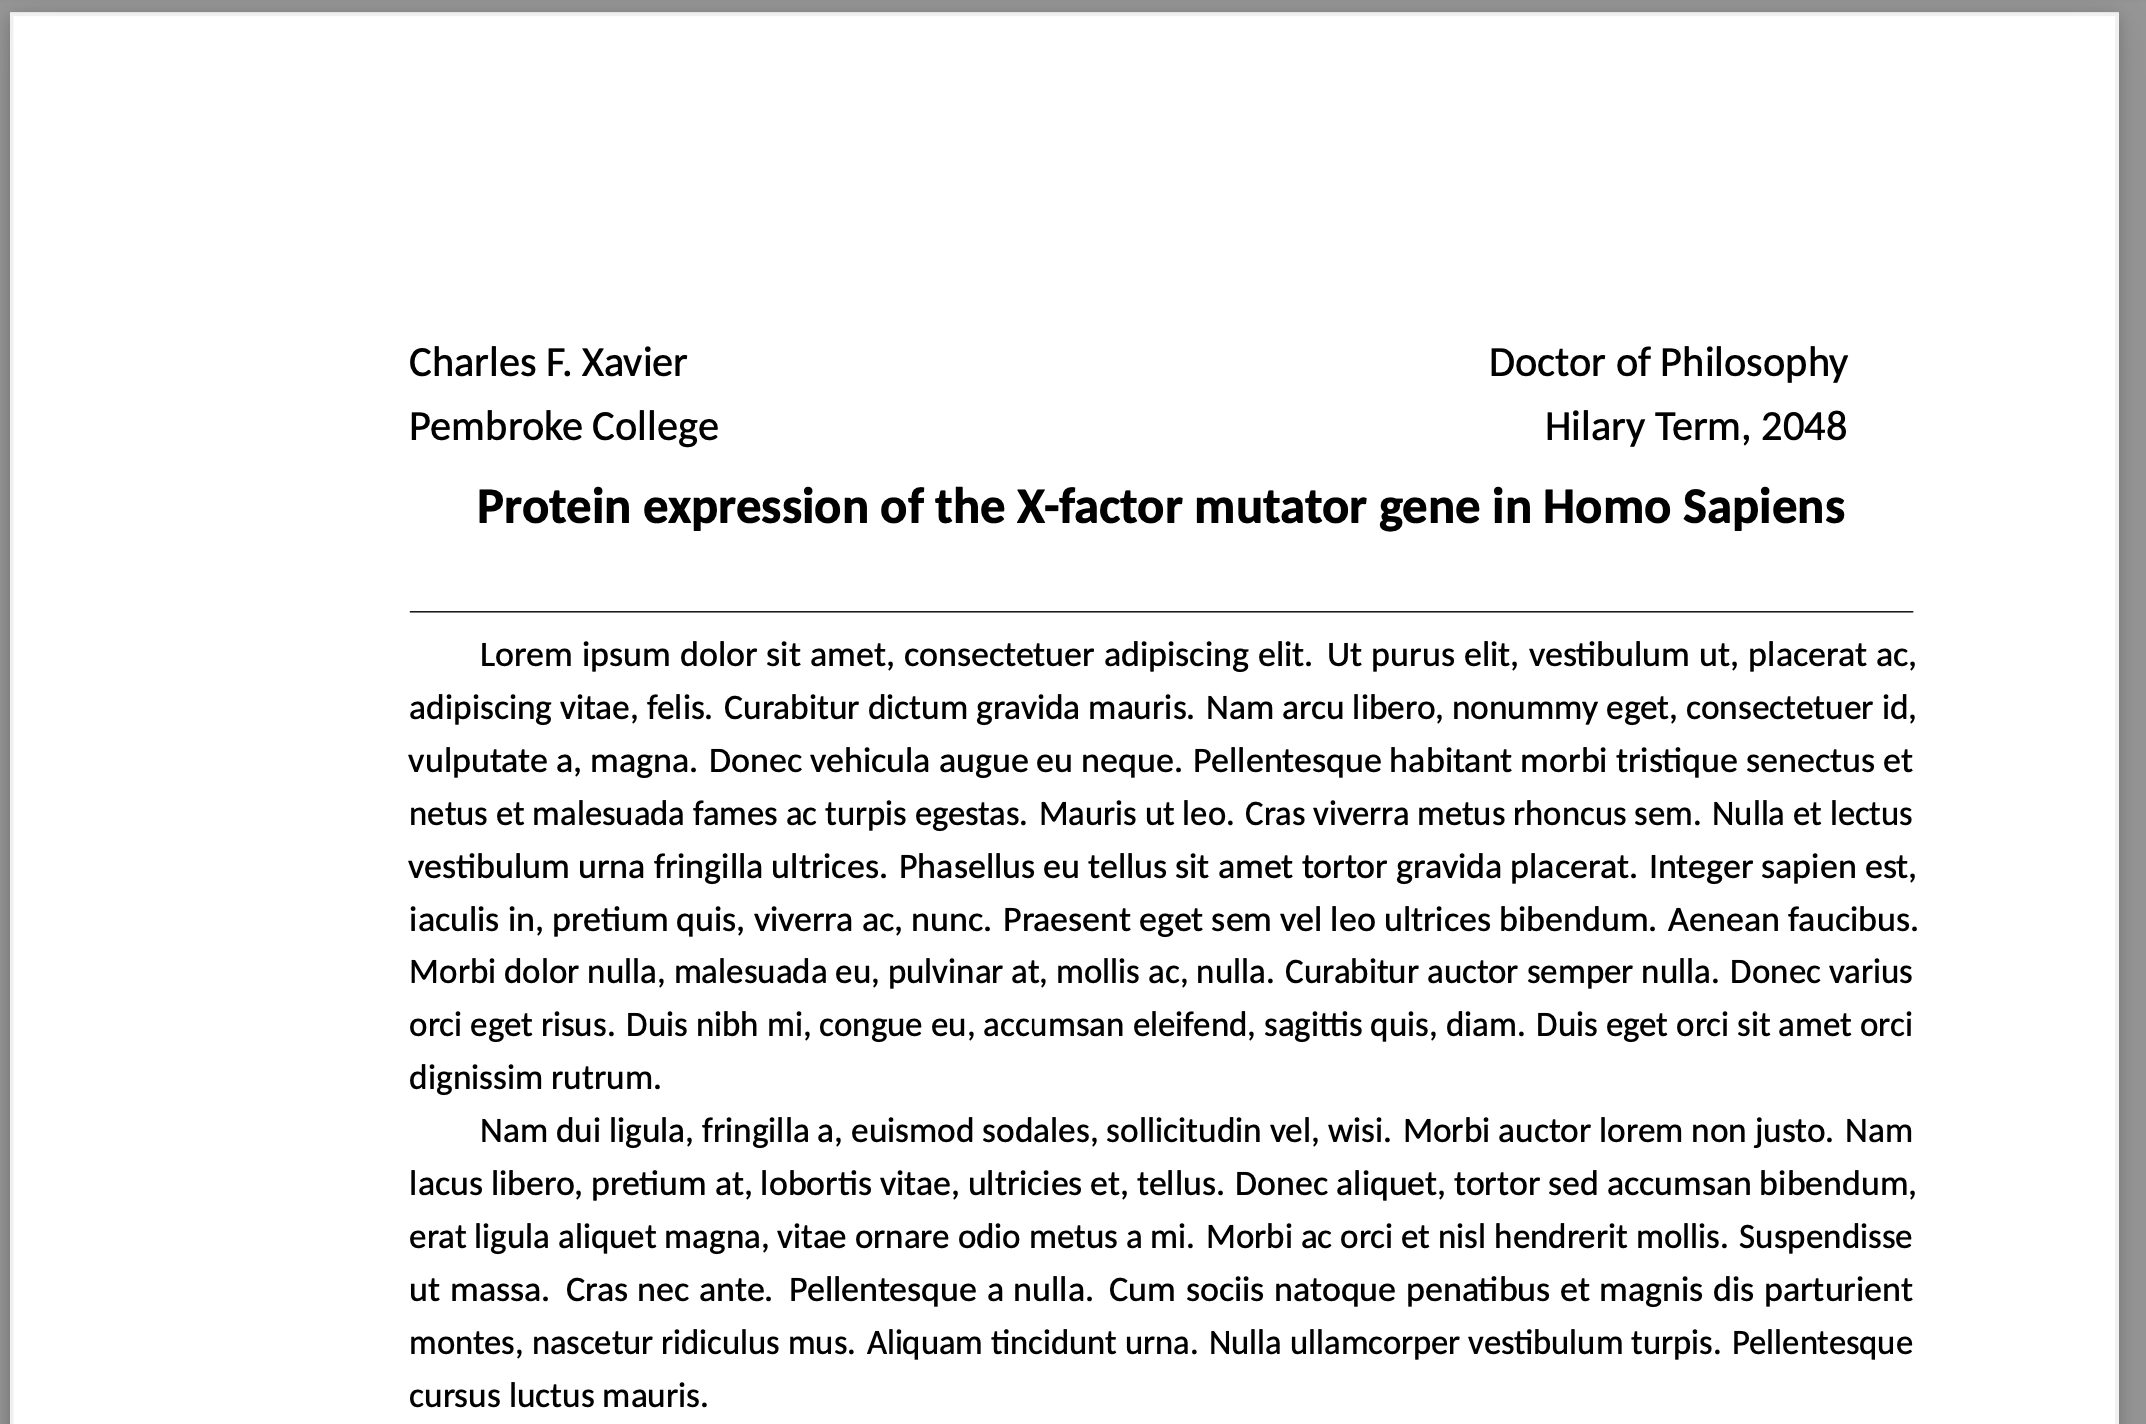
\includegraphics[width=0.7\linewidth]{dphil-front_abstract_page}
    \caption[Example of the abstract page for the Examination Schools]
    {
        Example of the abstract page for the Examination Schools.
        \label{fig:ch0:dphil-front_abstract_page}
    }
\end{figure}


\subsection{Review editing mode}


Your thesis supervisor may request you to print your document with double line spacing so he/she can correct your draft (the \textcolor{red}{red pen!}). You can simply add the ``\verb|review|'' option to your document:


\begin{lstlisting}[style=custom-latex]
\documentclass[review]{oxengthesis}
\end{lstlisting}


\subsection{Different colour for section headings}


The default font colour for section and subsection headings is black. You can change the colour (to blue for example) by adding the ``\verb|headingcolour|'' class option:


\begin{lstlisting}[style=custom-latex]
\documentclass[headingcolour={0.25,0.45,0.76}]{oxengthesis}
\end{lstlisting}


Note that the colour of \verb|\subsubsection| headings will be black regardless of the setting above.


\subsection{Chapter heading styles}


The default style for chapter headings is simple and gives you enough space to write your content. You can take advantage of different chapter styles defined in the \textit{memoir}\footnote{\url{https://ctan.org/pkg/memoir}} package by passing the ``\verb|chapterstyle|'' option. The code shown below will use the ``\verb|southall|'' chapter style to produce the sample \cref{fig:ch0:chapterstyle-southall}.


\begin{lstlisting}[style=custom-latex]
\documentclass[chapterstyle=southall]{oxengthesis}
\end{lstlisting}


\begin{figure}[htb]
    \centering
    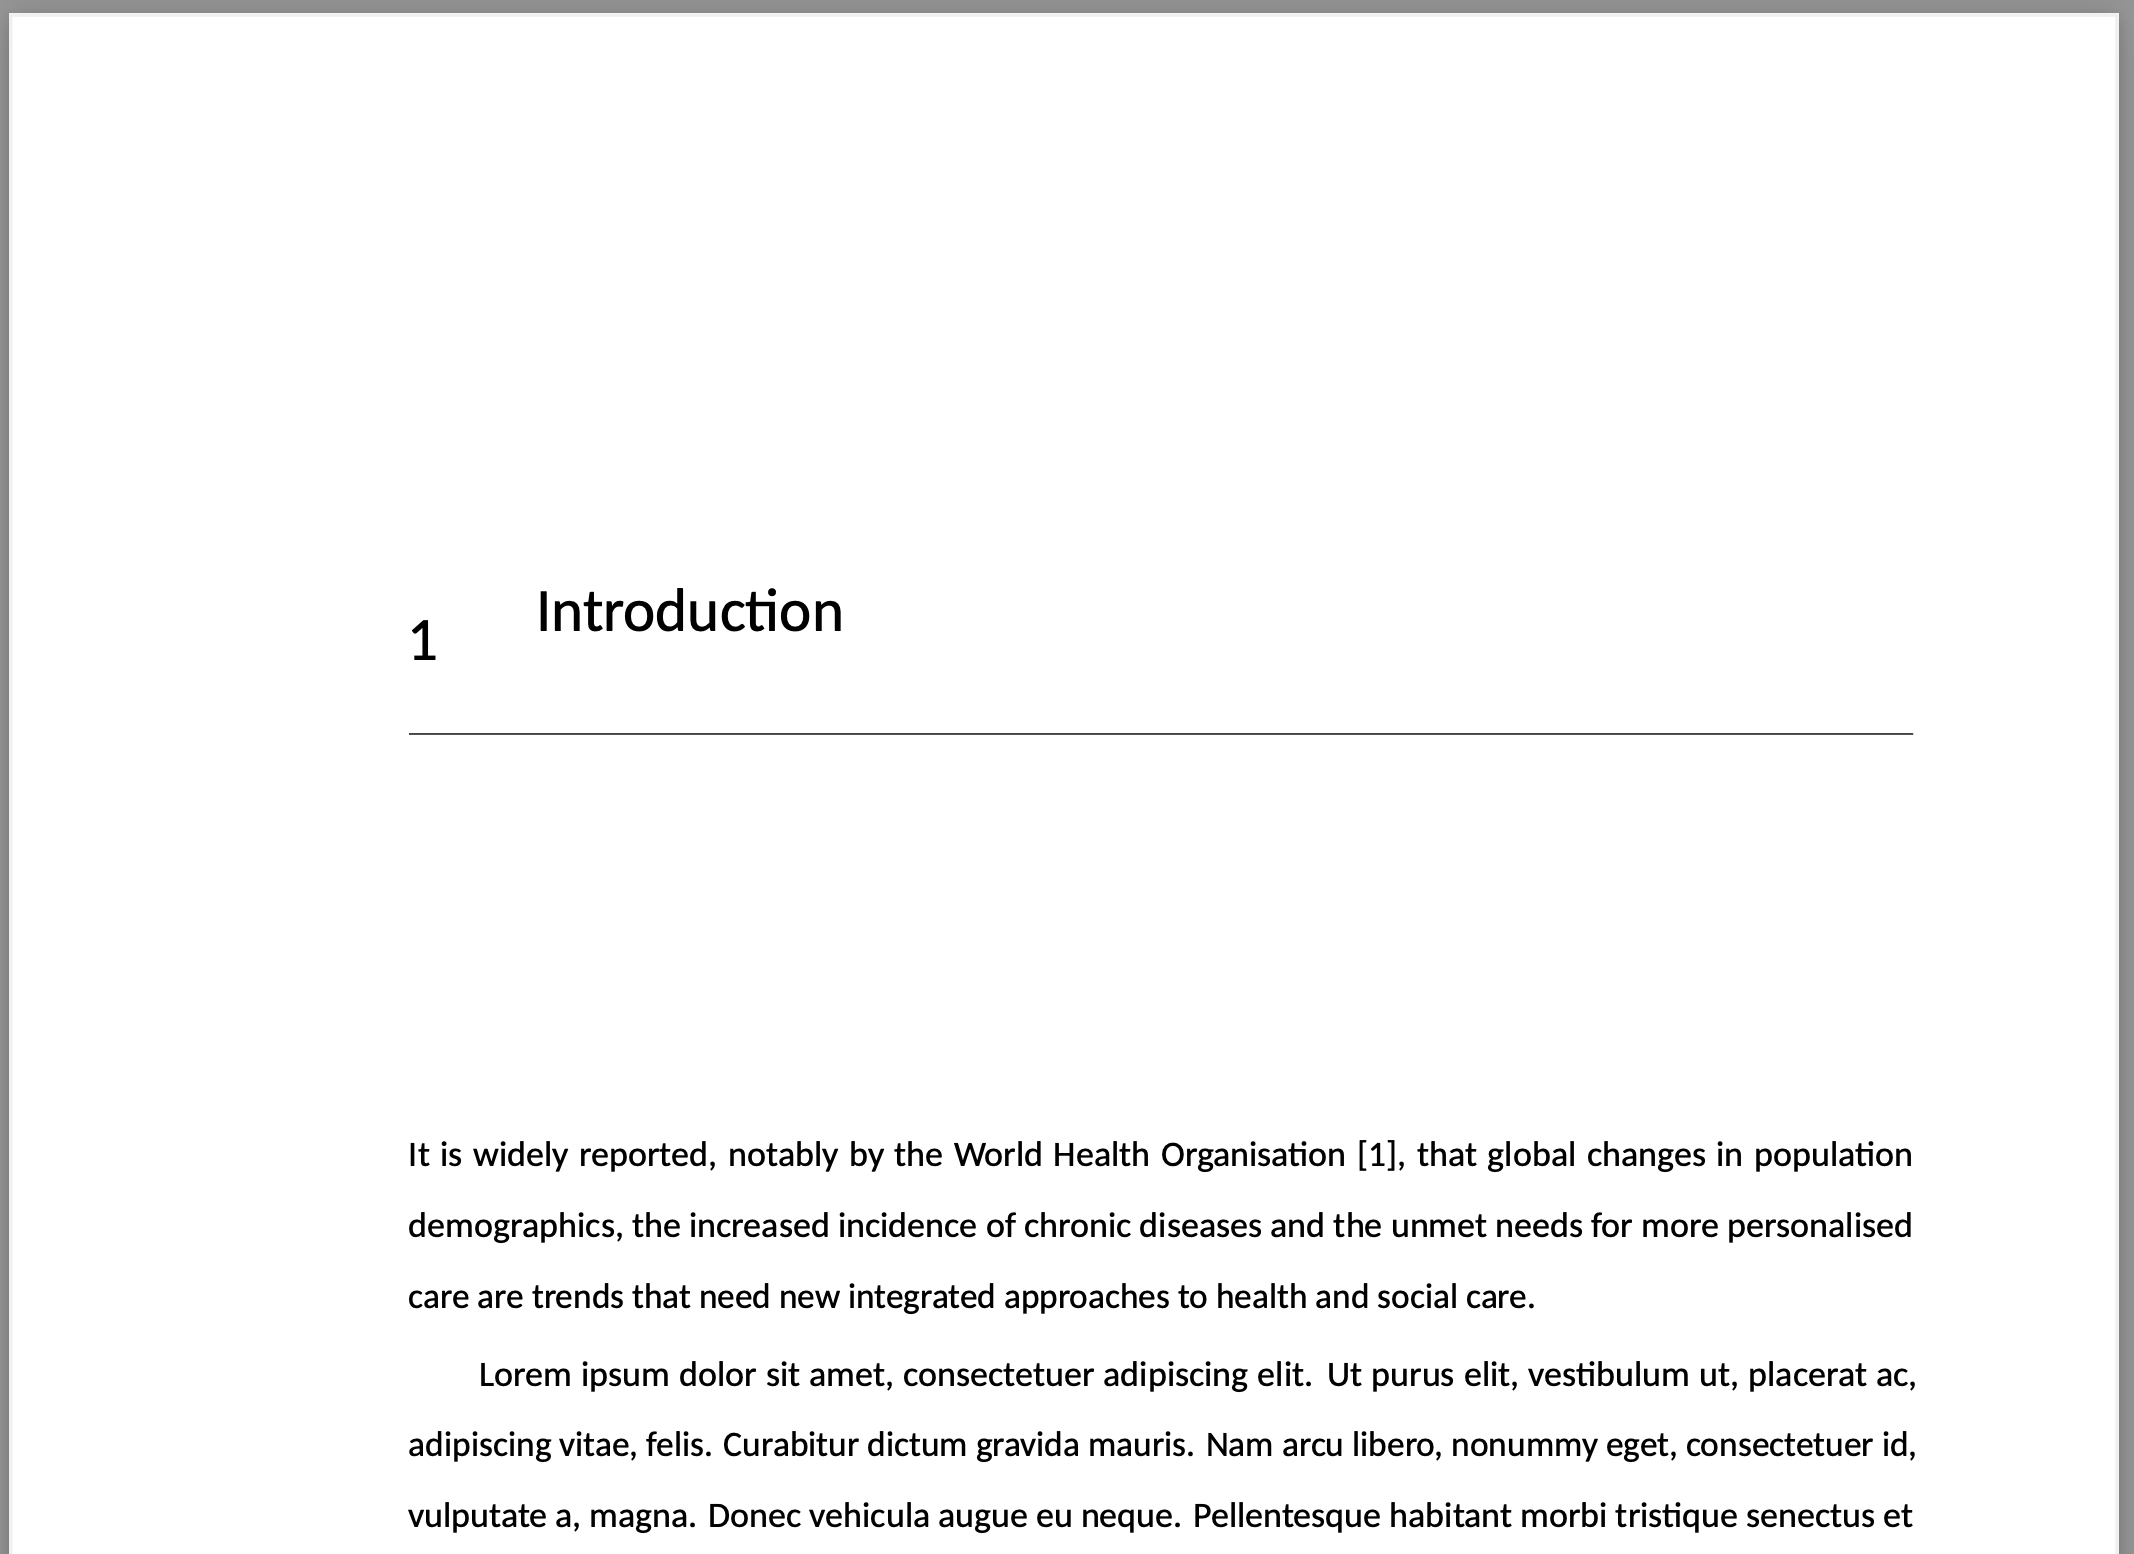
\includegraphics[width=0.7\linewidth]{chapterstyle-southall}
    \caption[The southall chapter heading style]
    {
        The southall chapter heading style.
        \label{fig:ch0:chapterstyle-southall}
    }
\end{figure}


\section{Additional features}


This section describes some of the additional features available in the OxEngThesis class. Refer to the official documentation of the \textit{memoir}\footnote{\url{https://ctan.org/pkg/memoir}} LaTeX package to customise your document even further.


\subsection{Figures}


\begin{figure}[htb]
    \centering
    \includegraphics[width=0.5\linewidth]{dummy_image}
    \caption[Sample figure covering 50\% of the page width]
    {
        Sample figure covering 50\% of the page width.
        \label{fig:ch0:sample_image}
    }
\end{figure}


I use the \textit{graphicx}\footnote{\url{https://ctan.org/pkg/graphicx}} package to include figures. You can put all figures in a ``\url{figures/}'' folder and you can simply include the image file directly without the file extension. For example, \cref{fig:ch0:sample_image} shows the image file ``\url{./figures/dummy_image.png}''. You can also create a figure with sub plots, as shown in \cref{fig:ch0:subfig_example}. Note that you can directly refer to the subplot as ``\cref{fig:ch0:subfig_example:fig1}''.


\begin{figure}
    \centering
    \subbottom[\label{fig:ch0:subfig_example:fig1}]{
        \includegraphics[width=0.3\linewidth]{dummy_image}
    }
    \subbottom[\label{fig:ch0:subfig_example:fig2}]{
        \includegraphics[width=0.3\linewidth]{dummy_image}
    }
    \subbottom[\label{fig:ch0:subfig_example:fig3}]{
        \includegraphics[width=0.3\linewidth]{dummy_image}
    }
    \caption[Sample figure with sub figures]
    {
        Sample figure with sub figures, showing:
        \subcaptionref{fig:ch0:subfig_example:fig1} caption for subfigure 1,
        \subcaptionref{fig:ch0:subfig_example:fig2} caption for subfigure 2 and
        \subcaptionref{fig:ch0:subfig_example:fig3} caption for subfigure 3.
        \label{fig:ch0:subfig_example}
    }
\end{figure}


\subsection{Tables}


\begin{table}[htb]
    \centering
    \caption{General features and specification for ...}
    \singleTableRowHeight
    \begin{tabular}{ll}

        \tableHeaderStart
        \tableHCell{Item} & \tableHCell{Description} \\
        \tableHeaderEnd

        Imaging Sensor        & Sony ICX625 2/3" progressive scan CCD \\
        Image size (pixels)   & 2448 (H) x 2048 (V)                   \\
        Pixel Size            & 3.45 \si{\micro\metre} x 3.45 \si{\micro\metre} \\
        A/D Converter         & AD9977 14-bit, dual-channel           \\
        Max frame rate        & 15 FPS                                \\
        Video Data Output     & 8, 12, 16 and 24-bit digital data     \\
        Gain \& Exposure                  & Automatic/Manual/One-Push \\
        Lens Mount            & C-mount                               \\
        Interface             & Gigabit Ethernet                      \\
        Physical dimensions   & 44 (W) mm x 29 (H) mm x 58 (L) mm     \\
        \hline 

    \end{tabular}
    \label{table:ch0:camera_specs}
\end{table}


You can create tables using the regular syntax in LaTeX. You can also create tables with additional styles. For example, \cref{table:ch0:camera_specs} shows a classical table with shaded headers. You can have more complex tables, as shown in \cref{table:ch0:patient_demographics}


\begin{table}[htb]
  \centering
  \caption{Summary of population demographics in the training and test sets}
  {
    \small
    \begin{tabular}{p{2cm} c c c c c c c c c c}
      \toprule

      Set &
      \multirowcell{2}{Number of\\subjects} &
      \multirowcell{2}{Total time\\(hours)}$^1$ &
      \multicolumn{2}{c}{Gender} &      
      \multicolumn{6}{c}{Ethnicity$^2$}  \\

      \cmidrule{4-11}
        
      &  &  & Male & Female & W & B & A & WB & WA & O  \\
      \midrule
      Training  & 15 & 216.6 & 8  & 7  & 10 & 1   & 1 & 1 & 1 & 1 \\        
      Test      & 15 & 210.0 & 10 & 5  & 10 & $-$ & 1 & 1 & 2 & 1 \\        
      \midrule        
      Total	& 30 & 426.6 & 18 & 12 & 20 & 1   & 2 & 2 & 3 & 2 \\
        
      \bottomrule
        
      \multicolumn{11}{l}
      {
        \footnotesize $^1$ Period during which both reference and estimated data were being recorded simultaneously.        
      } \\        
      \multicolumn{11}{l}
      {        
        \footnotesize $^2$ W = White, B = Black, A = Asian, WB = Mixed White \& Black, WA = Mixed White \& Asian and O = Other.        
      } \\
        
      \end{tabular}      
  } 
  \label{table:ch0:patient_demographics}
\end{table}


\subsection{Cross-referencing labels}


I use the \textit{cleveref}\footnote{\url{https://ctan.org/pkg/cleveref}} package to automatically format the label when cross referencing chapters, sections, figures and other common LaTeX labels. The following paragraphs, show some of the results.

You don't have to include the word ``chapter'': \Cref{chapter:literature_review} discusses .... is presented in \cref{chapter:dataset} with a detailed ...

You don't have to include the word ``figure'' or ``table'': The summary of the demographics for the entire set is described in \cref{table:ch0:patient_demographics} ... \Cref{fig:ch0:subfig_example} shows the video camera used in the study. \Cref{fig:ch0:subfig_example:fig1} shows the the camera model used, \cref{fig:ch0:subfig_example:fig2} shows the ... and \cref{fig:ch0:subfig_example:fig3} shows...


\subsection{Glossary, acronyms and abbreviations}


I use the \textit{glossaries-extra}\footnote{\url{https://ctan.org/pkg/glossaries-extra}} packages to define acronyms and automatically add the ``Glossary'' page in the \textit{frontmatter}. Simply create a file with the name ``glossary.tex'' and add all your definitions to it. Note that the first time you use an acronym, its full definition will be provided. For the rest of the instances, only the abbreviation will be used. The following paragraphs show how to define and use acronyms.

The standard vital signs include temperature, \ab{hr}, \ab{rr}, \ab{bp} and, when appropriate, \ab{spo2}. The routine measurement and interpretation of these vital signs is a core component of the physiological assessment of most patients \cite{prior1977physical,goldberg2005practical} as they can provide critical information about the underlying state of their health. 

We included all study types looking at monitoring of \ab{hr}, \ab{bp}, \ab{rr} or \ab{spo2} using image analysis with comparison to a reference device. We did not restrict based on clinical setting and included all age groups. Only non-contact methods using cameras were included. All unpublished studies found were included wherever possible to minimise publication bias.


\subsection{Citations and references}


This section contains example on how to cite papers, journals and other documents:

It is widely reported, notably by the World Health Organisation \cite{stroetmann2010can}, that global changes in population demographics, the increased incidence of chronic diseases and the unmet needs for more personalised care are trends that need new integrated approaches to health and social care. \cite{brooks1984infrared}


\lipsum[1]\cite{barker1987pulse,peacock1998oxygen,moller1993randomized}


Finding reliable correspondences in two images of a scene taken from arbitrary viewpoints viewed with possibly different cameras and in different illumination conditions is a difficult and critical step towards fully automatic reconstruction of 3D scenes\cite{hartley2003multiple}.


\lipsum[7]\cite{priya2012transition,haralick1973textural,Grass2012Online,NoninPulseOxOnline}


\subsection{Bibliography styles}


The default style for the references is ``\verb|ieeetr|''. For example, the following text: ``\textit{...Finding reliable correspondences in two images of a scene taken from arbitrary viewpoints viewed with possibly different cameras and in different illumination conditions is a difficult and critical step towards fully automatic reconstruction of 3D scenes \cite{hartley2003multiple}...}'' will produce the following output in the bibliography section at the end of the thesis:


\begin{lstlisting}[style=custom-text]
Bibliography
...
[8] R. Hartley and A. Zisserman, Multiple view geometry in computer vision. Cambridge university press, 2003.
...
\end{lstlisting}


You can specify a custom bibliography style as an argument to the ``\verb|\listofreferences|'' command in your \textit{main LaTeX source file}. For example, the following command:


\begin{lstlisting}[style=custom-latex]
\listofreferences[apalike]
\end{lstlisting}


\noindent will use the \textit{apalike}\footnote{\url{https://www.bibtex.com/s/bibliography-style-base-apalike}}
BibTeX style and produce the following output in the content pages:


\begin{lstlisting}[style=custom-text]
...Finding reliable correspondences in two images of a scene taken from arbitrary viewpoints viewed with possibly different cameras and in different illumination conditions is a difficult and critical step towards fully automatic reconstruction of 3D scenes [Hartley and Zisserman, 2003]...
\end{lstlisting}


\noindent and the bibliography section will read:


\begin{lstlisting}[style=custom-text]
Bibliography
...
[Hartley and Zisserman, 2003] Hartley, R. and Zisserman, A. (2003). Multiple view geometry in computer vision. Cambridge university press.
...
\end{lstlisting}

Take a look at the available styles at \textit{The quick BibTeX guide}\footnote{\url{https://www.bibtex.com/styles}} online.


\subsection{Mark text as TODO}


You can wrap text in``todo'' tags, so they appear in red colour in the PDF document. For example:

\todo{This text is in red colour, it reminds me of a task to complete}


\subsection{Formatting source code}


Often, we want to show pseudo code, source code or other verbatim content in our document. For this, I use the \textit{listings}\footnote{\url{https://ctan.org/pkg/listings}} package. The extra custom styles defined in the OxEngThesis class file are:


Example on displaying C/C++ source code:


\begin{lstlisting}[style=custom-c,caption={Function to balance a matrix.}]
extern PE_SIGPROC_API void pesig_balance(
        const size_t    n,
        signal_value_t  A[n][n],
        signal_value_t* S
        );
\end{lstlisting}


Example on displaying BASH/Console scripts:


\begin{lstlisting}[style=custom-bash,caption={A script in bash.}]
$ mkdir -p $HOME/code/pebase/realtime
$ cd $HOME/code/pebase/realtime
$ git clone git@github.com:maurovm/thesis_template.git repository
\end{lstlisting}


Example of displaying text as ``verbatim'' mode:


\begin{lstlisting}[style=custom-verbatim,caption={License information.}]
OxEngThesis is provided under:

    SPDX-License-Identifier:    GPL-2.0-only
    
OxEngThesis is free software: you can redistribute it or modify
it under the terms of the GNU General Public License as published by the
Free Software Foundation, version 2 only, according with:

    LICENSES/GPL-2.0

OxEngThesis is distributed in the hope that it will be useful, but
WITHOUT ANY WARRANTY; without even the implied warranty of MERCHANTABILITY
or FITNESS FOR A PARTICULAR PURPOSE. See the GNU General Public License
for more details.
\end{lstlisting}


\subsection{Coloured boxes}


I use the \textit{tcolorbox}\footnote{\url{https://ctan.org/pkg/tcolorbox}} package to show coloured and framed text boxes with an optional heading line. Some examples include:

\noindent Standard box:


\begin{tcolorbox}
\lipsum[1]
\end{tcolorbox}


\noindent Standard box with title:


\begin{tcolorbox}[title=Box title]
\lipsum[1]
\end{tcolorbox}


\noindent A small box following text:\dotfill\tcbox[nobeforeafter,colframe=blue!50!black,colback=white,colupper=red!50!black]{Hello World}\hfill


Read the documentation of the \verb|tcolorbox| package to see an extensive description of the configuration options and what you can do with the \verb|tcolorbox| class, it is quite customisable. The OxEngThesis class defines some environment commands for some predefined boxes. For example, the following is a warning box:


\begin{OxWarningBox}{Warning box title}
Warning box content: \lipsum[1]
\end{OxWarningBox}


The following example shows an information box:


\begin{OxInfoBox}{Informational box title}
Warning box content: \lipsum[1]
\end{OxInfoBox}


\section{Troubleshooting common errors}


\subsection{Text beyond page limits}


When compiling a LaTeX document, you could get a warning similar to:


\begin{lstlisting}[style=custom-text]
Overfull \hbox (22.49216pt too wide) in paragraph at lines 4--5
\end{lstlisting}


This often occurs when a line of your document could not fit within the designated horizontal space for text in the current page layout. The LaTeX compiler tries its best to fit text within the page limits, but sometimes it just cannot do it appropriately. This typically results in some text hanging out past the page margin due to long words, acronyms or long equations. Sometimes, it is difficult to know where these errors occur in your document. You can add the ``\verb|debuglayout|'' option to your document:


\begin{lstlisting}[style=custom-latex]
\documentclass[debuglayout]{oxengthesis}
\end{lstlisting}


\begin{figure}[htb]
    \centering
    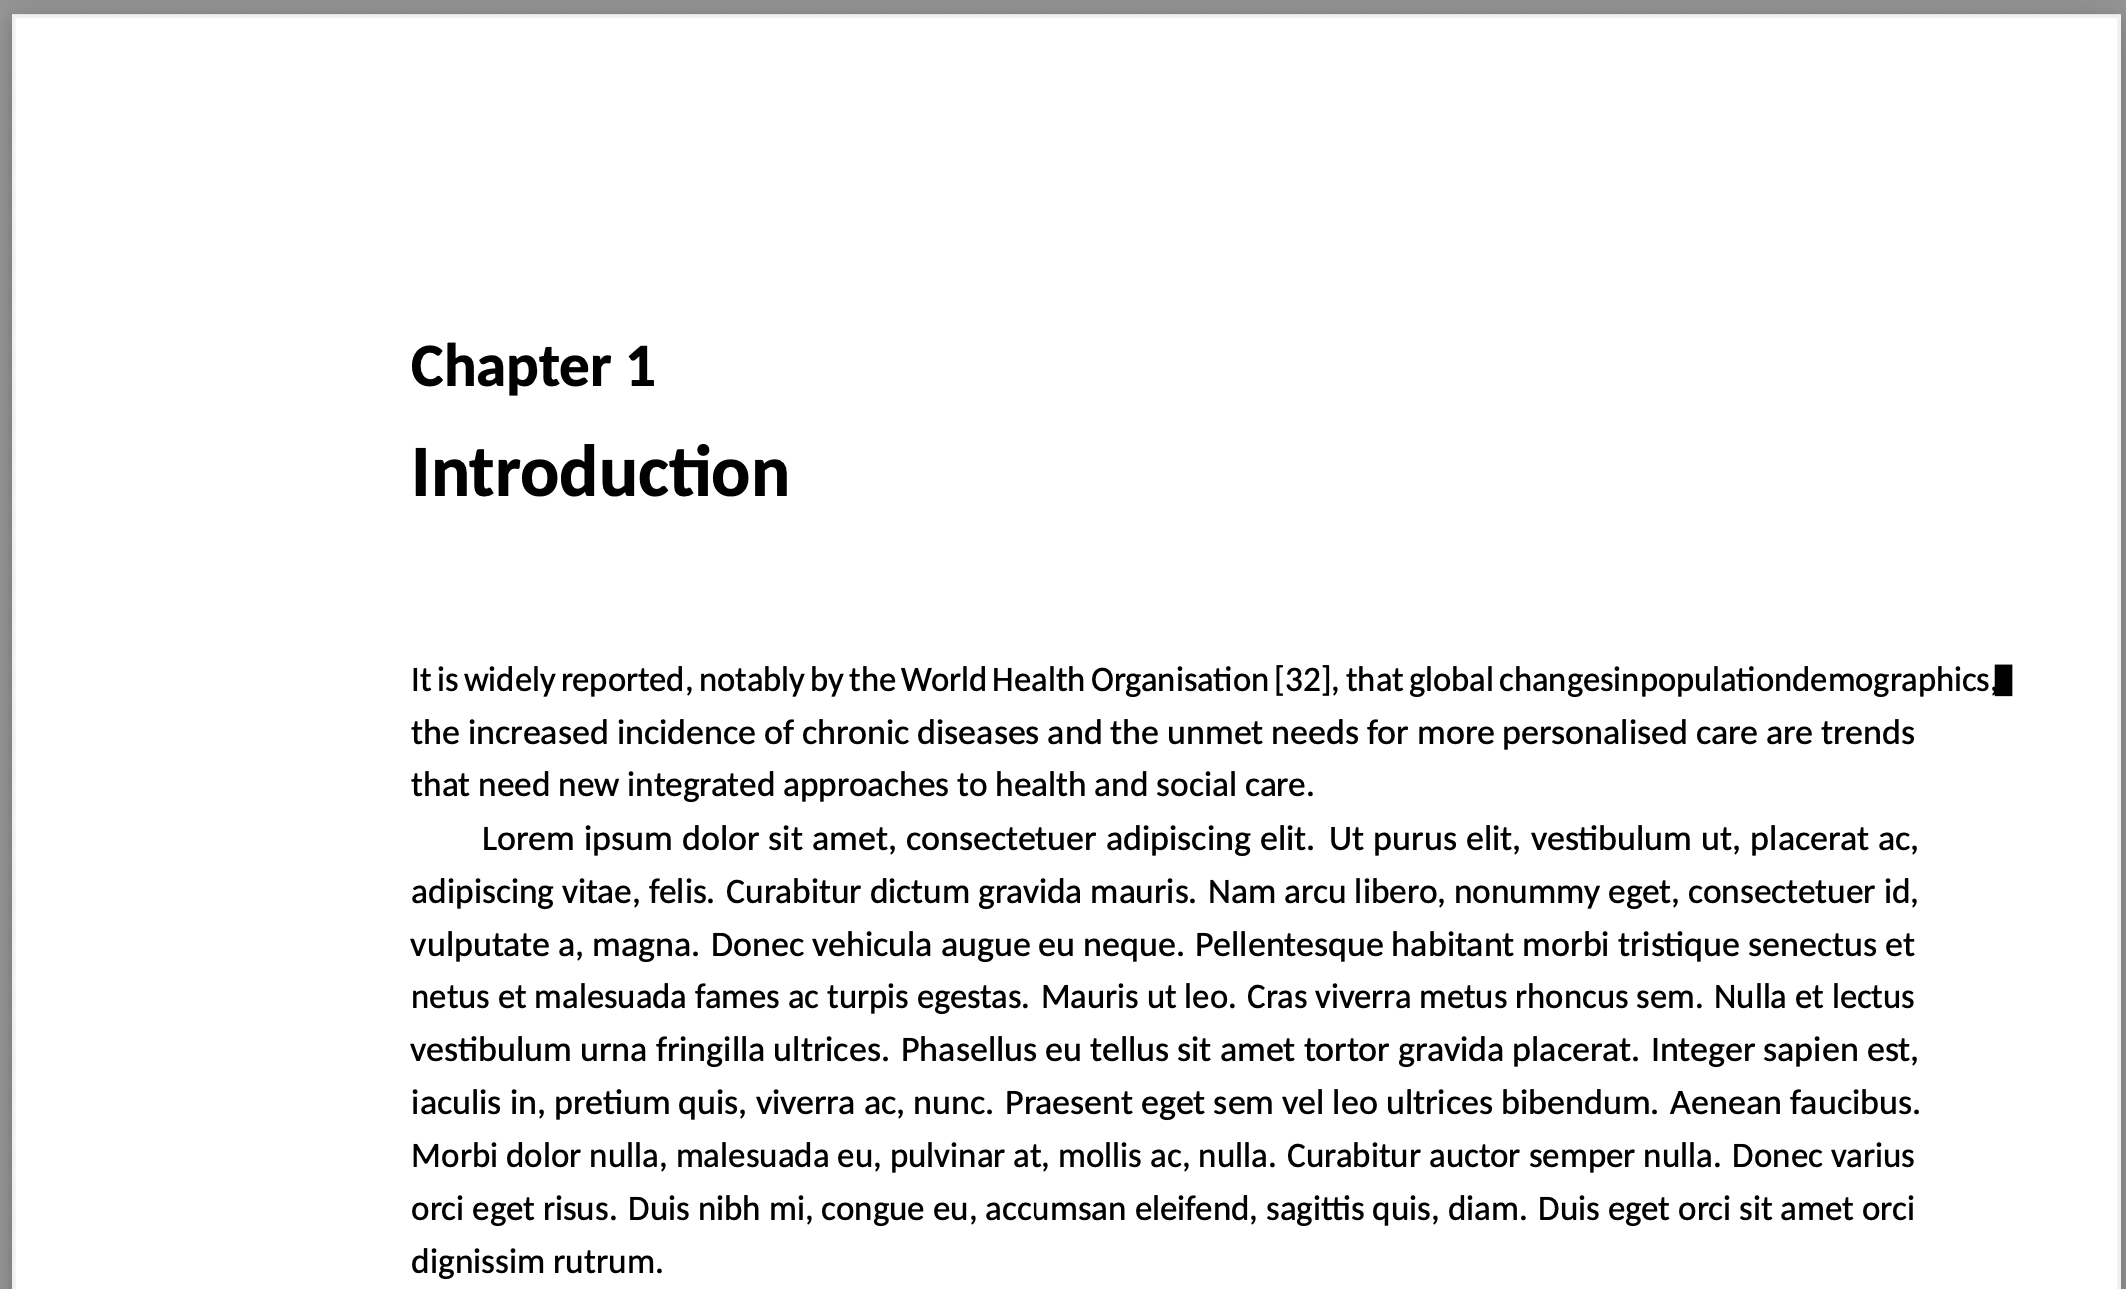
\includegraphics[width=0.7\linewidth]{overfull_hbox_warning}
    \caption[Example of a line of text that does not fit within the horizontal space for text]
    {
        Example of a line of text that does not fit within the horizontal space for text. A black box is shown next to the affected line.
        \label{fig:ch0:overfull_hbox_warning}
    }
\end{figure}


A black box will be shown next to the affected lines, as shown in \cref{fig:ch0:overfull_hbox_warning}. The \url{oxengthesis.cls} class file already takes advantage of other packages (such as \textit{microtype}\footnote{https://ctan.org/pkg/microtype}) to deal with common issues such as character protrusion, font expansion and inter-word spacing. I recommend you slightly rephrase your guilty sentences instead of changing the class template. This is usually the first approach many of my students take.




\chapter{Introduction}
\label{chapter:introduction}

It is widely reported, notably by the World Health Organisation \cite{stroetmann2010can}, that global changes in population demographics, the increased incidence of chronic diseases and the unmet needs for more personalised care are trends that need new integrated approaches to health and social care.

\lipsum[1-2]\cite{brooks1984infrared}

\lipsum[3-4]\cite{barker1987pulse,peacock1998oxygen,moller1993randomized}

\section{Monitoring of vital signs}

The standard vital signs include temperature, \af{hr}, \af{rr}, blood pressure and, when appropriate, \af{spo2}. The routine measurement and interpretation of these vital signs is a core component of the physiological assessment of most patients \cite{prior1977physical,goldberg2005practical}, as they can provide critical information about the underlying state of their health. Finding reliable correspondences in two images of a scene taken from arbitrary viewpoints viewed with possibly different cameras and in different illumination conditions is a difficult and critical step towards fully automatic reconstruction of 3D scenes\cite{hartley2003multiple}.

\lipsum[7-11]\cite{priya2012transition,haralick1973textural,Grass2012Online,NoninPulseOxOnline}

\section{Clinical need}

\lipsum[1-2]\cite{HidalgoEquivitalEQ02Online,poh2011advancements,poh2010non,verkruysse2008remote,wieringa2005contactless,wiki:bayerfilter,nonin9560oem,Mas_Fernandez_2003,hartley2003multiple}

\subsection{sub section 1}

\lipsum[3-6]\cite{schmidt1997animal,4036907,Orbanz2008,varjavand2002interactive,report:PCESC2005,HSU_05_2012,collins2015relating,abdi2010principal}

\subsection{sub section 2}

\lipsum[10-12]\cite{cote1988effect,aravindhan2000sulfhemoglobinemia,clayton1991pulse,clayton1991comparison,webb1991potential,212885,964165,Chaichulee2017FG}

\section{Objectives}

\lipsum[2-4]

\section{Contributions}

\lipsum[2-4]

\section{Outline of document}

\Cref{chapter:literature_review} discusses .... . The clinical study undertaken as part of this project is presented in \Cref{chapter:dataset} with a detailed description of the patient population, the data collection process and an overview of the main vital signs used as the reference data....

\lipsum[2-4]

\chapter{Spectra in the atmosphere}
\label{chapter:literature_review} 


\section{Introduction}

\section{Spectra in turbulence theory}

\subsection{Kolmogorov's -5/3 spectrum}

\begin{itemize}

\item{Simple explanation for the existence of the scaling range}

\item{The log correction}

\item{Observation of the law}

\item{Simulation}

\end{itemize}

\subsection{Spectra in 2D turbulence}

\begin{itemize}

\item{Simple explanation for scaling ranges and directions of energy flux}

\item{Log corrections?}

\item{Observations of the law}

\item{Simulations of the law}

\end{itemize}

\subsection{Spectra and predictability}

\begin{itemize}

\item{Simple explanation of why energy at a scale is associated with the predictability time}

\item{Explanation of the finite time barrier of predictability}

\end{itemize}

\subsection{Methods of calculating the spectrum}

\begin{itemize}

\item{2D Fourier transform, exact formula and fact that you use Parseval and so square after}

\item{1D lines and the translation between them and the spectra, highlight importance}

\item{Structure functions and their link to the spectrum}

\item{Spherical harmonics and the translation between degree and wavenumber}

\item{Mention of wavelet techniques, this is a subcategory of coarse-graining which is addressed in detail in the second chapter and will not be expanded on here}

\end{itemize}

\section{Spectra in observations}

\subsection{First observations and historical context}

\begin{itemize}

\item{Nastrom and Gage}

\item{The idea of the energy gap and implications for predictability}

\end{itemize}

\subsection{Current observations}

\begin{itemize}

\item{The variablity of the slope with height, include that figure you made from the analysis that was novel in its presentation and cite all that one paper that had change with height}

\item{The direction of energy flux and why it matters}

\item{Variability rather than universality}

\end{itemize}

\section{Spectra in simulations}

\subsection{The effects of resolution}

\subsection{Aquaplanets and such}

\section{Theoretical explanations of the spectrum}

\subsection{The synoptic scale spectrum}

\begin{itemize}

\item{Charney and -3 and such}

\item{Other caveats}

\end{itemize}

\subsection{The mesoscale spectrum}

\subsubsection{Not 3D turbulence}

\subsubsection{2D inverse cascade}

\subsubsection{2D direct cascade}

\subsubsection{Wave wave interactions}

\subsubsection{Wave mean interactions}

\subsubsection{Direct imprinting}

\subsubsection{Stratified turbulence}


\chapter{Coarse-graining}
\label{chapter:method} 


\section{Introduction}

\begin{itemize}

\item{The idea of coarse graining in brief}

\end{itemize}

\section{Relationship with Fourier spectrum}

\begin{itemize}

\item{Show random noise with spectrum that top hat can resolve, compare spectra}

\item{Introduce integral relation between coarse-grain and Fourier spectrum}

\item{Show random noise top hat cannot resolve to motivate order}

\end{itemize}

\section{Concept of order}

\begin{itemize}

\item{Define order of a kernel}

\item{show higher order kernel difference in resolving one from previous section}

\item{Show how order can be used to show that will tend to the right slope}

\end{itemize}

\section{Extension to the sphere}

\begin{itemize}

\item{Just explain how concepts generalise to the sphere}

\end{itemize}

\section{Extension to vector fields}

\begin{itemize}

\item{Simple explanation of why Helmholtz is so useful}

\end{itemize}

\section{The coarse-grain energy flux}

\section{Note on the relationship with wavelets}



\chapter{Local spectra}
\label{chapter:results} 


\section{Maps of local spectra in the atmosphere}

\begin{itemize}
		
\item Analysis, what it is, why we used it

\textbf{The Dataset}

Analysis refers to an estimate of the current state of the atmosphere. Its production is a key step of numerical weather prediction since it provides the initial conditions from which the forecasts can be run. It is usually produced through the combination of simulated and observational data in a process called data assimilation. The analysis dataset we use in this thesis is the \gls{ecmwf}, \gls{ifs} operational analysis.

Reanalysis refers to the production of these best guesses for the atmospheric state for times in the past. They are usually produced at a lower resolution than analysis but have the advantage of using a single model, whereas the model used to produce analysis is often upgraded. One of the most widely used reanalyses currently is the \gls{era5}.

Our goal was to investigate the global mesoscale atmospheric state in a way that best reflected our current knowledge of that state. The widely used heuristic for effective resolution is eight times the grid resolution \cite{skamarock2004evaluating}. In ERA5, the grid resolution is around 25 km so the estimated effective resolution is 200~km. In practice this means most of the mesoscales are unresolved and indeed the spectral characteristics of the mesoscales are either not reproduced or difficult to detect \cite{li2023intercomparison}. By contrast, the ECMWF IFS operational analysis provides a high-resolution ($\sfrac{1}{12}^\circ$, estimated effective resolution of 70~km) dataset that still assimilates observational data. This operational analysis demonstrates a clear shallowing that agrees well with high-resolution global simulations \cite{Wang2021a, stephan2022atmospheric}. 

We analysed the whole of 2020, with hourly means sampled 4 times per day at 00, 06, 12 and 18 UTC. This study was confined to the 200 and 600~hPa pressure levels. Precipitation and orography data were sourced from ERA5 for 2020 \cite{hersbach2020era5}. Although the ECMWF model changes frequently, in 2020 it only changed once in June, the impact of this change on our analysis was found to be minimal. 

\item{Global spectra}

\textbf{Comparison with spherical harmonics over the same period}

Figure \ref{fig:ch4:SphvsFiltSpec} shows a comparison of the spherical harmonic and filtering spectrum over 2020 in the analysis. In our data analysis we resolved the filter spectrum up to a filtering scale of 1000~km. As discussed in [CITE PART OF METHOD CHAPTER] we expect to see some differences between the two spectra, in particular the filtering spectrum can be viewed as a spectrally local average of the Fourier spectrum. In addition, there is no reason for the filter scale and the corresponding wavenumber to exactly coincide. Given these considerations, Figure \ref{fig:ch4:SphvsFiltSpec} demonstrates a good agreement between the two methods, showing that general trends in slope are indeed reproduced. The resolved mesoscales in the operational analysis are indicated with red dashed lines.  

\begin{figure}[htb]
    \centering
    \includegraphics[width=\linewidth]{Chap4/SphvsFiltSpecCombined.pdf}
    \caption[A comparison of the spherical harmonic spectrum and the filtering spectrum.]
    {
        The average spherical harmonic spectrum for 2020 compared with the average filtering spectrum for 600 hPa (left) and 200 hPa (right). 
        \label{fig:ch4:SphvsFiltSpec}
    }
\end{figure}

\item{Rotational vs divergent motion}

Figure \ref{fig:ch4:RotDivSpec} shows the spectrum of the rotational (horizontally divergence-free) and divergent (irrotational) components of the global spectrum for 2020. This is obtained by performing a Helmholtz decomposition on the flow and then finding the filtering spectrum associated with the resulting divergence-free and curl-free components.

While a Helmholtz decomposition is not strictly a wave decomposition, the divergent component strongly aligns with geostrophically unbalanced motion, mostly consisting of gravity waves at our scales, and the rotational with balanced motions \cite{morfa_avalos_2024,waite2020untangling}. 

\begin{figure}[htb]
    \centering
    \includegraphics[width=\linewidth]{Chap4/RotDivSpec.pdf}
    \caption[Rotational and divergent components of the global filtering spectrum.]
    {
        The average filtering spectrum for 2020 decomposed into rotational (blue) and divergent (red) components for 600 hPa (left) and 200 hPa (right). 
        \label{fig:ch4:RotDivSpec}
    }
\end{figure}

\item{Global spectra with Rotational divergent decomposition}

\item{Map of spectral slopes}

\item{Map showing relative KE of divergent and rotational component}

\item{Map showing rotational and divergent slopes in different locations}

\item{Show map of mesoscale energy flux}

\item{Bootstrapping}

\item{Map showing bootstrap variance of spectral slope}
		
\end{itemize}

\section{Conditioned maps}

\begin{itemize}

\item{We explain in detail what conditioned spectra are in chap 2 but in brief...}

\item{Seemed clear that spectra are strongly influenced by convective events, conditioning on precipitation... }

\item{We can further explore this by breaking down into lsp and cp}

\item{Show aggregate energy fluxes for lsp and cp}

\item{This is an energy aggregate, if we were to consider the spectrum at a particular point at a particular time no guarantee a spectral slope would make sense}

\item{However, let us assume such a slope does make sense. What is the average slope we observe, in other words, the non energy weighted slope.}

\item{Show scatter plot of slope vs tp, lsp and cp}

\item{Show a plot of average aggregate spectral slope vs average measured daily slope}

\item{Show slopes conditioned on Orography, mention how ice sheets are excluded due to their unique nature}

\item{Show energy fluxes conditioned on orography}

\item{Talk about how spectra conditioned on surface gradient were disappointing and speculate this is due to the gradient being at an irrelevant scale}

\item{Speculate on how boundary layer investigation could be interesting, conditioned on surface roughness, wind shear, surface temperature and stratification}

\item{Show slopes conditioned on Flux direction}

\item{Speculate about how this could bring back older theories}

\item{Show PI conditioned on direction of energy flux}

\item{Show spectra for different energy flux amounts - more money in the economy so more energy, little difference in slope}

\item{Aggregate energy flux based on the slope of the energy spectrum, do steeper slopes associate with more large scale to small scale flux?}

\item{Why divergent mesoscale energy is a proxy for gravity wave activity}

\item{Condition spectra based on mesoscale div KE}

\item{Condition spectra based on the ratio of Div to Rot KE}

\item{Condition energy flux based on ratio of Div to Rot KE}

\item{Condition spectra based on the surface level pressure}

\item{Condition energy flux based on this, point out that difference in crossover scale may be different characteristic sizes of low and high pressure systems}

\item{Condition spectra by removing precip and land}

\item{Decompose into Rot Div and argue that majority of effect comes from divergent motions}

\end{itemize}

\section{Variability}

\begin{itemize}

\item{Condition spectra by season}

\item{Show global map for each season}

\item{Condition spectra by time of day}

\item{Show global map for each time of day}

\item{Condition spectra by latitude}

\item{Show latitude on x axis, slope on y axis, aggregate and measured}

\end{itemize}

\section{Spectra in ERA5}

\begin{itemize}

\item{Why we don't dwell on ERA5}

\item{Broad patterns are consistent}

\item{Show ERA5 map of spectral slopes}

\end{itemize}

\section{Conclusions}

\begin{itemize}

\item{The importance of multiple perspectives}

\item{We have made it clear that not just downscale is relevant}

\item{Slope has a strong dependence on meteorological conditions}

\item{Variability in slope is in need of an explanation}

\item{Differences in the spectra for different directions of energy flux are in need of explanation}

\item{We can quantify energy transfer in different meteorological situations, this could be interesting for blocking and range of other phenomena}

\item{For a more extended discussion of possible future work, see the next chapter}

\end{itemize}





\chapter{Further applications}
\label{chapter:future_work} 

\section{Introduction}

\begin{itemize}

\item{This consists of more speculative work}

\end{itemize}

\section{Explaining the spectrum}

\begin{itemize}

\item{Looking at longer time series}

\item{Looking at signals of atmospheric phenomena}

\item{Doing a coarse-grain break down of the energy flux and diagnosing local relative importance of different stuff}

\end{itemize}

\section{Model evaluation}

\subsection{Local effective resolution}

\subsection{Enhancing spectra for model improvement validation}

\begin{itemize}

\item{Can reference current use of spectra for model evaluation}

\item{Can mention that particular use case of AI forecasts}

\end{itemize}

\section{Predictability}

\subsection{Ensemble spread and the spectra of initial conditions}

\subsection{Conditioned error spectra in idealised simulations}

\subsection{Conditioned error spectra in GCMs}

\begin{itemize}

\item{Local error saturation time}

\item{Local measure of upscale vs cascade error growth}

\item{Also may help address problem of in inconsistent metrics in combination with feature tracking}

\end{itemize}






\chapter{Conclusion}
\label{chapter:conclusion} 

\begin{itemize}

\item{We have presented a novel framework}

\item{We have shown x y z}

\item{We envision}

\end{itemize}



%\bibliography{references.bib}
%\appendix

%\chapter{Bayesian change point detection}
\label{appendix:appendix_1} 


To estimate the location of a step change, a Bayesian change point detection algorithm based on \cite{Ruanaidh1996} and \cite{adams2007bayesian} is used in the thesis. Given a data sequence $x$ of $N$ samples with Gaussian noise added:

\begin{equation}
    \centering
      x_i=\begin{cases}
          \mu_1 + \epsilon_i, & \text{if $i<m$}.\\
          \mu_2 + \epsilon_i, & \text{otherwise}.
          \end{cases}
    \label{eq:app:cp:5.1}
\end{equation}

where the noise samples $\epsilon_i$ are assumed to be independent and $m$ is the step change location. The likelihood of the data is given by the joint probability of the noise samples $\epsilon_i$: 

\begin{equation}
    \centering
    P(x|\{\mu_1\mu_2\sigma m\}) = \prod\limits_{i=1}^N P(\epsilon_i)
    \label{eq:app:cp:5.2}
\end{equation}

where $\sigma$ is the standard deviation of the Gaussian noise;  $\mu_1, \mu_2$ and $\sigma m$ are the known time series parameters. The probability density function for the noise samples is defined by:

\begin{equation}
    \centering
    P(\epsilon) = \frac{1}{\sigma \sqrt{2 \pi} }  e ^{ - \frac{ (\epsilon - \mu)^2 } {2\sigma^2} }
    \label{eq:app:cp:noise_pdf}
\end{equation}

\lipsum[12-17]
%\chapter{Optical flow estimation}
\label{appendix:appendix_2} 


\lipsum[2-9]


\backmatter 
\listofreferences[apalike]

\end{document}
